\documentclass[iicol,sn-basic]{sn-jnl}

\jyear{2021}%

%% as per the requirement new theorem styles can be included as shown below
\theoremstyle{thmstyleone}%
\newtheorem{theorem}{Theorem}%  meant for continuous numbers
%%\newtheorem{theorem}{Theorem}[section]% meant for sectionwise numbers
%% optional argument [theorem] produces theorem numbering sequence instead of independent numbers for Proposition
\newtheorem{proposition}[theorem]{Proposition}% 
%%\newtheorem{proposition}{Proposition}% to get separate numbers for theorem and proposition etc.

\theoremstyle{thmstyletwo}%
\newtheorem{example}{Example}%
\newtheorem{remark}{Remark}%

\theoremstyle{thmstylethree}%
\newtheorem{definition}{Definition}%

\raggedbottom
%%\unnumbered% uncomment this for unnumbered level heads
% If your paper is accepted, change the options for the package
% aistats2021 as follows:
%
%\usepackage[accepted]{aistats2021}
%
% This option will print headings for the title of your paper and
% headings for the authors names, plus a copyright note at the end of
% the first column of the first page.

% If you set papersize explicitly, activate the following three lines:
%\special{papersize = 8.5in, 11in}
%\setlength{\pdfpageheight}{11in}
%\setlength{\pdfpagewidth}{8.5in}

% If you use natbib package, activate the following three lines:
%\usepackage[round]{natbib}
%\renewcommand{\bibname}{References}
%\renewcommand{\bibsection}{\subsubsection*{\bibname}}

% If you use BibTeX in apalike style, activate the following line:
%\bibliographystyle{apalike}
%\usepackage[noend]{algpseudocode}
\raggedbottom
%%\unnumbered% uncomment this for unnumbered level heads
\usepackage{graphicx}
\usepackage{amsmath}
\usepackage{amssymb}

% Include other packages here, before hyperref.

% If you comment hyperref and then uncomment it, you should delete
% egpaper.aux before re-running latex.  (Or just hit 'q' on the first latex
% run, let it finish, and you should be clear).

%\usepackage{cuted}
%Theorems
%\usepackage{amsthm} % before newtxmath because of \openbox

%\usepackage{mathtools}
%\mathtoolsset{showonlyrefs}

\usepackage{color}

%%% Input encoding
\usepackage[utf8]{inputenc}
\usepackage{microtype}      % microtypography
%%% Fonts
\usepackage[T1]{fontenc}
%\usepackage[vvarbb]{newtxmath}
\usepackage{booktabs}       % professional-quality tables


\usepackage{etoolbox}
\usepackage[enable]{easy-todo}

% For nice subfigures
\usepackage{graphicx}
%\usepackage{subcaption}
\usepackage{multirow}

\usepackage{subfig}
%\usepackage{tabstackengine}
%\useackage{enumitem}
%\usepackage[section]{placeins}

\usepackage{algorithm}
\usepackage{algpseudocode}

\usepackage{comment}
\usepackage{adjustbox}

%\usepackage{apacite}
\let\R\relax
\newcommand*{\R}{\mathbb{R}}
\newcommand*{\Po}{\text{Prox}}
\newcommand*{\Am}{\text{argmin}}
\newcommand*{\E}{\mathbb{E}}
\newcommand*{\VRG}{\,\tilde{\nabla}_k^s}
\newcommand{\norm}[1]{\left\lVert#1\right\rVert}
\newcommand{\Iprod}[2]{\left\langle #1,#2\right\rangle}
\newcommand\myeq[2]{\mathrel{\stackrel{{{#1}}}{#2}}}
\newcommand{\abs}[1]{\vert#1\vert}

\renewcommand{\algorithmicrequire}{
\textbf{Input:}}
\renewcommand{\algorithmicensure}{\textbf{Output:}}
\newcommand{\Initialize}{\textbf{Initialize:}{\,}}
\newcommand{\Input}{\textbf{Input:}{\,}}
\newcommand{\Output}{\textbf{Output:}{\,}}

\newtheorem{lemma}[theorem]{Lemma}
\newtheorem{conjecture}[theorem]{Conjecture}
\newtheorem{condition}[theorem]{Condition}
\newtheorem{claim}[theorem]{Claim}
\newtheorem{question}[theorem]{Question}
\newtheorem{corollary}[theorem]{Corollary} 
\newtheorem{statement}[theorem]{Statement}
\newtheorem{notation}[theorem]{Notation} 
\newtheorem{assumption}{Assumption}
\setcounter{secnumdepth}{0}  
\newcommand{\keepcomment}{1}% Remove comment
\AtBeginDocument{\ifnum\keepcomment=1
  \excludecomment{comment}
\else
  \includecomment{comment}
\fi}
\allowdisplaybreaks
%include only supp materials
%\includeonly{sub}

\begin{document}

% If your paper is accepted and the title of your paper is very long,
% the style will print as headings an error message. Use the following
% command to supply a shorter title of your paper so that it can be
% used as headings.
%
%\runningtitle{I use this title instead because the last one was very long}

% If your paper is accepted and the number of authors is large, the
% style will print as headings an error message. Use the following
% command to supply a shorter version of the authors names so that
% they can be used as headings (for example, use only the surnames)
%
%\runningauthor{Surname 1, Surname 2, Surname 3, ...., Surname n}
\title[Article Title]{Efficient Zeroth-Order Proximal Stochastic Method for Nonconvex Nonsmooth Black-Box Problems}

%%=============================================================%%
%% Prefix	-> \pfx{Dr}
%% GivenName	-> \fnm{Joergen W.}
%% Particle	-> \spfx{van der} -> surname prefix
%% FamilyName	-> \sur{Ploeg}
%% Suffix	-> \sfx{IV}
%% NatureName	-> \tanm{Poet Laureate} -> Title after name
%% Degrees	-> \dgr{MSc, PhD}
%% \author*[1,2]{\pfx{Dr} \fnm{Joergen W.} \spfx{van der} \sur{Ploeg} \sfx{IV} \tanm{Poet Laureate} 
%%                 \dgr{MSc, PhD}}\email{iauthor@gmail.com}
%%=============================================================%%

\author*[1]{\fnm{Ehsan} \sur{Kazemi}}\email{ehsan\_kazemy@knights.ucf.edu}

\author[1]{\fnm{Liqiang} \sur{Wang}}\email{lwang@cs.ucf.edu}

\affil[1]{\orgdiv{Department of Computer Science}, \orgname{University of Central Florida}}



%%==================================%%
%% sample for unstructured abstract %%
%%==================================%%

\abstract{Proximal gradient method has a major role in solving nonsmooth composite optimization problems. However, in some machine learning problems related to black-box optimization models, the proximal gradient method could not be leveraged as the derivation of explicit gradients are difficult or entirely infeasible. Several variants of zeroth-order (ZO) stochastic variance reduced such as ZO-SVRG and ZO-SPIDER algorithms have recently been studied for nonconvex optimization problems. However, almost all the existing ZO-type algorithms suffer from a slowdown and increase in function query complexities up to a small-degree polynomial of the problem size. In order to fill this void, we propose a new analysis for the stochastic gradient algorithm for optimizing nonconvex, nonsmooth finite-sum problems, called ZO-PSVRG+ and ZO-PSPIDER+. The main goal of this work is to present an analysis that brings the convergence analysis for ZO-PSVRG+ and ZO-PSPIDER+ into uniformity, recovering several existing convergence results for arbitrary minibatch sizes while improving the complexity of their ZO oracle and proximal oracle calls. We prove that the studied ZO algorithms under Polyak-Łojasiewicz condition in contrast to the existent ZO-type methods obtain a global linear convergence for a wide range of minibatch sizes when the iterate enters into a local PL region without restart and algorithmic modification. The current analysis in the literature is mainly limited to large minibatch sizes, rendering the existing methods unpractical for real-world problems due to limited computational capacity. In the empirical experiments for black-box models, we show that the new analysis provides superior performance and faster convergence to a solution of nonconvex nonsmooth problems compared to the existing ZO-type methods as they suffer from small-level stepsizes. As a byproduct, the proposed analysis is generic and can be exploited to the other variants of gradient-free variance reduction methods aiming to make them more efficient.}

%%================================%%
%% Sample for structured abstract %%
%%================================%%

% \abstract{\textbf{Purpose:} The abstract serves both as a general introduction to the topic and as a brief, non-technical summary of the main results and their implications. The abstract must not include subheadings (unless expressly permitted in the journal's Instructions to Authors), equations or citations. As a guide the abstract should not exceed 200 words. Most journals do not set a hard limit however authors are advised to check the author instructions for the journal they are submitting to.
% 
% \textbf{Methods:} The abstract serves both as a general introduction to the topic and as a brief, non-technical summary of the main results and their implications. The abstract must not include subheadings (unless expressly permitted in the journal's Instructions to Authors), equations or citations. As a guide the abstract should not exceed 200 words. Most journals do not set a hard limit however authors are advised to check the author instructions for the journal they are submitting to.
% 
% \textbf{Results:} The abstract serves both as a general introduction to the topic and as a brief, non-technical summary of the main results and their implications. The abstract must not include subheadings (unless expressly permitted in the journal's Instructions to Authors), equations or citations. As a guide the abstract should not exceed 200 words. Most journals do not set a hard limit however authors are advised to check the author instructions for the journal they are submitting to.
% 
% \textbf{Conclusion:} The abstract serves both as a general introduction to the topic and as a brief, non-technical summary of the main results and their implications. The abstract must not include subheadings (unless expressly permitted in the journal's Instructions to Authors), equations or citations. As a guide the abstract should not exceed 200 words. Most journals do not set a hard limit however authors are advised to check the author instructions for the journal they are submitting to.}


%%\pacs[JEL Classification]{D8, H51}

%%\pacs[MSC Classification]{35A01, 65L10, 65L12, 65L20, 65L70}

\keywords{Nonconvex optimization, Zeroth-order methods, Polyak-Łojasiewicz condition, Nonsmooth optimization, Query efficient methods, Adversarial attacks}


\maketitle
% \onecolumn
%main draft
\section{Introduction}
In this paper, we consider nonsmooth nonconvex optimization problems of the generic form
\begin{equation}\label{problem}
\min_{x\in\R^d} F(x) =  f(x) + h(x),\,\,\,f(x):=\frac{1}{n}\sum_{i=1}^n f_i(x)
\end{equation}
where each $f_i(x)$ is possibly nonconvex and smooth function, and $h(x)$ is a nonsmooth convex function such as $L_1$-norm regularizer. 
The optimization problem \eqref{problem} governs
numerous machine learning frameworks, ranging from neural networks to  generalized linear models and from convex problems like SVM and Lasso to highly nonconvex optimization problems such as loss functions tailored to deep neural models. In this work, we shall explore a set of variance-reduced stochastic zeroth-order (SZO) optimization algorithms for \eqref{problem} to improve their oracle calls. Stochastic variance-reduced gradient (SVRG) is a powerful approach to decrease the variance inherited from stochastic sampling \cite{johnson2013accelerating,reddi2016stochastic,nitanda2016accelerated,allen2016improved}. These papers demonstrate that SVRG enhances the rate of convergence for stochastic gradient descent (SGD) by a factor of $O(1/{\epsilon})$ due to the decrease in the variance of the gradient. The underlying idea to develop zeroth-order variance reduction methods is to leverage similar ideas from the first-order methods to reduce the variance of stochastic optimization methods in order to improve the convergence rate. The major adversity of first-order methods is their dependency on first-order information from the problem, while there are settings where the first-order gradients are computationally infeasible or costly whereas zeroth-order information (function information) is accessible. For instance, in online auctions and advertisement
selections, only zeroth-order information in the form of responses to the queries is accessible \cite{wibisono2012finite}. This illustrates the importance of the development of zeroth-order optimization methods for solving many machine-learning problems. Currently, there are only a few zeroth-order stochastic methods
for solving problem \eqref{problem}, e.g., \cite{ghadimi2016mini} and \cite{huang2019faster}. \cite{ghadimi2016mini} introduced a gradient-free proximal projection (RSPGF) algorithm using a two-point Gaussian random gradient estimator for smooth composite optimization problem \eqref{problem}, which achieves a convergence rate of
$O(\sqrt{d}/\sqrt{T})$ with $T$ is the number of iterations) and stochastic zeroth-order query complexity of $O(\frac{d^2}{\epsilon^2})$, to reach a stationary point $x^*$ such that $\norm{F(x^*)} \leq \epsilon$. There are other variants of zeroth-order for nonsmooth problems, e.g., \cite{huang2019faster} and also momentum accelerated zeroth-order methods \cite{chen2019zo} to achieve a higher rate of convergence. In addition, several zeroth-order projection-free methods were developed in \cite{sahu2019towards, huang2020accelerated} as well as ADAM-based methods in \cite{gao2018information}.

The other variation of variance reduction optimization schemes was introduced in \cite{fang2018spider} called SPIDER. Being different from SVRG-type algorithms, SPIDER \cite{fang2018spider} and the earlier version \cite{nguyen2017sarah,nguyen2017stochastic} are first-order stochastic variance-reduced schemes where in each inner-loop iteration gradient is estimated recursively by applying the variance-reduced gradient estimation in the past iteration (see \eqref{spider-grad-fo}). A zeroth-order variant of SPIDER was proposed in \cite{fang2018spider}, named SPIDER-SZO. This set of ZO variance-reduced methods replaces first-order gradients in the SPIDER algorithm with zeroth-order gradient estimators. In \cite{fang2018spider} it shows that SPIDER-SZO gains an improved zeroth-order query complexity compared to SVRG-based zeroth-order algorithms. Nevertheless, the original SPIDER-SZO algorithm requires generating a large number of Gaussian random samples of order $O(n^{1/2}d^2)$ at each epoch and the convergence guarantee is obtained with a stepsize of $O(\epsilon)$. In practice, these requirements significantly limit the performance of SPIDER-SZO.


Recently, \cite{ji2019improved} refined the ZO estimations to derive an improved SZO complexity with improved convergence rates. However, the analysis in their work is only for smooth functions based on a complicated parameter selection analysis which is only valid for particular and mainly large minibatch sizes. Towards improving the convergence analysis in the existing works, in this paper we address this open question: {\it Is this possible to extend the existing convergence analysis for ZO-SVRG and ZO-SPIDER to arbitrary minibatch sizes with improved ZO query complexity and under more general nonsmooth, nonconvex setting?} Aiming to answer this question, we employ variance reduction methods to design an accelerated ZO proximal method for nonsmooth composite optimization problem \eqref{problem}. This demonstrates an improvement to ZO iteration complexity up to a factor of ${d}$ compared with \cite{huang2019faster} and extends the existing analysis for ZO variance-reduced framework to versatile studies which are valid for more general parameter settings. 

In Tables \ref{table-compare} and \ref{table-compare-spider}, we compared the results from our analysis and other state-of-the-art ZO optimization methods for three different items. We also listed the minibatch sizes that our methods can achieve the optimal SZO calls known in the literature. Table \ref{table-compare} shows that the convergence of ZO-PSVRG+
provides a better dependency on problem dimension $d$ than RSPGF and ZO-ProxSVRG/SAGA for nonconvex nonsmooth optimization. It also shows that RGF has the largest query complexity yet has the worst convergence rate. ZO-SVRG-Coord and ZO-ProxSVRG/SAGA provide an improved rate of convergence $O(d/\epsilon )$ owning to applying variance reduction techniques. Further observation of Table \ref{table-compare} reveals that the existing SVRG type zeroth-order algorithms are highly affected by function query complexities compared to RSPGF, while ZO-PSVRG+ (our algorithm) could achieve better trade-offs between the convergence rate and the querying complexity. 
\section{Main Contributions}
In this work, we present a novel uniform analysis for ZO-PSVRG+ (Algorithm \ref{APGnonconvex-Algo}) and ZO-PSPIDER+ (Algorithm \ref{spider-APGnonconvex-Algo}) which are different from the comparable convergence studies. Although recently several accelerated variance reduction techniques for nonconvex problems have been proposed \cite{wang2019spiderboost}, in this work we mainly focus to improve the analysis of the basic aforesaid methods and the extension to the novel accelerated frameworks shall be addressed in our future studies. 
The main contributions of this paper are summarized in the following:

1) Our analysis for ZO-PSVRG+ yields iteration complexity $O(\frac{1}{{\epsilon}})$ compared to $O(\frac{d}{\epsilon^2})$ of RSPGF \cite{ghadimi2016accelerated}  and $O(\frac{d}{\epsilon})$ of ZO-ProxSVRG/SAGA  \cite{huang2019faster} (the existing variance-reduce SZO proximal algorithm for solving nonconvex nonsmooth problems).  
It shows that our results have improved the complexity of the terms dependent on
$d$ in contrast to the existing proximal variance-reduced SZO methods. ZO-PSVRG+ also matches the best result achieved by ZO-SVRG-Coord-Rand with minibatch size $b = d n^{2/3}$ and epoch size $m = n^{1/3}$ in \cite{ji2019improved}, while our analysis is valid for {\it any minibatch sizes} as detailed in the following sections. In addition, our analysis ZO-PSPIDER+ for is superior compared to SPIDER-SZO \cite{fang2018spider} by entirely removing the requirement for i.i.d. Gaussian samples and permitting a larger stepsize $O(1)$ to enable a speedier convergence. These convergence advantages are due to a new  analysis that we present throughout this work. As seen from Figure \ref{order_conv_analysis-fig}, our analyses for both algorithms are valid for the entire range of minibatch sizes i.e., $b \in [1, n]$

2) The convergence analysis for ZO-PSVRG+ in contrast to  ZO-SVRG-Coord \cite{liu2018zeroth, ji2019improved} is straightforward and yields simpler proofs. Our analysis achieves new iteration complexity bounds and improves the effectiveness of all the existing ZO-SVRG-based algorithms along with RSPGF for nonconvex nonsmooth composite optimization. Note that the convergence studies for RSPGF and ZO-ProxSVRG/SAGA rely on bounded gradient assumption, which is not our working assumption in this paper.

3) For the nonconvex functions under the Polyak-Łojasiewicz (PL) condition \cite{polyak1963gradient}, we show that ZO-PSVRG+ and ZO-PSPIDER+
obtain a global linear convergence rate equivalent to the first-order ProxSVRG. Thus, these algorithms can certainly achieve linear convergence in some zones without restarting. To the best of
our knowledge, this is the first paper that leverages the PL condition for improving the convergence of the zeroth-order proximal variance-reduced method for problem \eqref{problem} with arbitrary minibatch sizes. This analysis generalizes the results \cite{duchi2015optimal} while showing linear convergence in contrast to the sublinear convergence rate in their paper.
In \cite{ji2019improved}, the authors show that  ZO-SPIDER-Coord achieves linear convergence under PL condition but the analysis is limited to the minibatch of size $b = O(n^{1/2})$. Note that due to both computational and statistical efficiency, convergence analysis for minibatch of moderate sizes is essential (also see the remarks after Theorem \ref{PL-Zoo-rand} for more details). 

Finally, to demonstrate the efficiency and adaptability of our approach in achieving a balance between the convergence rate and the number of SZO queries, we perform some
experimental evaluations for two distinct applications: black-box binary classification and universal adversarial
attacks on black-box deep neural network models. The empirical results and
theoretical investigations verify the effectiveness of our algorithms. To present the results coherently, 
we postpone our proofs for convergence analysis to the supplementary materials.

\begin{table*}[htb!]
 \centering
\caption{Summary of convergence rate and function query complexity of various SZO algorithms. S: Smooth, NS: Nonsmooth, NC: Nonconvex, C: Convex, SC: Strong Convexity, and PL: Polyak-Łojasiewicz Condition. $b$ denotes the minibatch size, $m$ denotes the epoch size, $T$ is the total number of iterations, $\lambda$ is the constant in PL condition \eqref{zo-pl-cond} and $s_n = \min\{n, \frac{1}{\epsilon}\}$. The dash-line ``-'' shows that the result is valid for a generic $b$ or $m$.}
\label{table-compare}
% \begin{adjustbox}{width=1.8\columnwidth,center}
\begin{adjustbox}{width=1.\linewidth,center}
{
\begin{tabular}{ |l|l|l|l|l|l|l| } 
 \hline
 Method & Problem & Stepsize& Convergence rate & SZO complexity & $b$ & $m$\\ 
 \hline
 ZO-GD (\cite{nesterov2011random}) & S(NC) & $O\left(\frac{1}{d}\right)$ & $O\left(\frac{d}{T}\right)$ &$O\left(\frac{dn}{\epsilon}\right)$ & NA & NA \\
 ZO-SGD (\cite{ghadimi2013stochastic}) & S(NC) & $O\left(\frac{1}{d}\right)$ & $O\left(\frac{\sqrt{d}}{\sqrt{T}}\right)$ &$O\left(\frac{d}{\epsilon^2}\right)$ & NA & NA\\ 
 RSPGF (\cite{ghadimi2016mini}) & S(NC) + S(C) & $O\left(1\right)$ & $O\left(\frac{\sqrt{d}}{\sqrt{T}}\right)$ &$O\left(\frac{d^2}{\epsilon^2}\right)$ & - & 1\\
 ZO-SVRG-Coord (\cite{liu2018zeroth}) & S(NC)& $O\left(\frac{1}{{d}}\right)$ & $O\left(\frac{d}{T}\right)$ & $O(\frac{nd^2}{\epsilon}+\frac{d^2b}{\epsilon})$ & - & $O(d)$ \\
 ZO-SVRG-Coord-Rand (\cite{ji2019improved}) & S(NC) & $O\left(\frac{1}{{dn^{2/3}}}\right)$ & $O\left(\frac{dn^{2/3}}{T}\right)$ & $O(\min\{\frac{dn^{2/3}}{\epsilon},\frac{d}{\epsilon^{5/3}}\})$ & $\mathcal{B}^{2/3}$ & $\mathcal{B}^{1/3}$ \\
%  ZO-SVRG-Coord-Rand (\cite{ji2019improved}) & S(NC)& $O\left(\frac{1}{{dn^{2/3}}}\right)$ & $O\left(\frac{dn^{2/3}}{T}\right)$ & $O(\min\{\frac{dn^{2/3}}{\epsilon},\frac{d}{\epsilon^{5/3}}\})$ & $1$ & $\mathcal{B}\,d$ \\
  ZO-ProxSVRG-Coord (\cite{huang2019faster}) & S(NC)+NS(C) & $O\left(\frac{1}{{d}}\right)$ & $O\left(\frac{d}{T}\right)$ &  $O(\frac{nd^2}{\epsilon\sqrt{b}}+\frac{md^2\sqrt{b}}{\epsilon})$ & $\mathcal{B}^{2/3}$ & $\mathcal{B}^{1/3}$\\
   ZO-ProxSAGA-Coord (\cite{huang2019faster}) & S(NC)+NS(C)& $O\left(\frac{1}{{d}}\right)$ & $O\left(\frac{d}{T}\right)$ & $O(\frac{(n + b)d^2}{\epsilon})$ & $\mathcal{B}^{2/3}$ & $\mathcal{B}^{1/3}$ \\
   ZO-PSVRG+ (Ours)  & S(NC)+NS(C) & $\eta = \min\{\frac{1}{8L}, \frac{\sqrt{b}}{12mL}\}$ & $O\left(\frac{1}{\eta T}\right)$ &  $O\left(\frac{\mathcal{B}d}{\epsilon\eta m}+\frac{bd}{\epsilon\eta}\right)$ & - & -\\
   &  & $\min\{\frac{1}{8L}, \frac{\sqrt{1}}{12L}\}$ & $O\left(\frac{1}{T}\right)$ &  $O\left(\min\{\frac{dn^{2/3}}{\epsilon},\frac{d}{\epsilon^{5/3}}\}\right)$ & $\mathcal{B}^{2/3}$ & $\mathcal{B}^{1/3}$ \\
   ZO-PSVRG+ (RandSGE) (Ours)  & S(NC)+NS(C) & $\eta = \min\{\frac{1}{8L}, \frac{\sqrt{b}}{12mL\sqrt{d}}\}$ & $O\left(\frac{1}{\eta T}\right)$ & $O\left(s_n\frac{d\sqrt{d}}{\epsilon \sqrt{b}}+\frac{b\sqrt{d}}{\epsilon}\right)$ & - & -\\
   ZO-PSVRG+ (Ours) & S(PL)+NS(C) & $\eta = \min\{\frac{1}{8L}, \frac{\sqrt{\gamma b}}{12 m L }\}$ & $O\left(\epsilon\right)$ & {$O(\frac{s_n d}{\lambda\eta m}\log\frac{1}{\epsilon}+\frac{b d}{\lambda\eta}\log\frac{1}{\epsilon})$} & - & - \\
   &  & $O(1)$ & $O\left(\epsilon\right)$ & $O(\min\{\frac{dn^{2/3}}{\lambda}\log\frac{1}{\epsilon},\frac{d}{\lambda\epsilon^{2/3}}\log\frac{1}{\epsilon}\})$ & $\mathcal{B}^{2/3}$ & $\mathcal{B}^{1/3}$ \\
   &  & $O(\frac{1}{m})$ & $O\left(\epsilon\right)$ & {$O(\min\{\frac{dn}{\lambda}\log\frac{1}{\epsilon},\frac{d}{\lambda\epsilon}\log\frac{1}{\epsilon}\})$} & 1 & - \\
   ZO-PSVRG+ (RandSGE) (Ours) & S(PL)+NS(C) & $\eta = \min\{\frac{1}{8L}, \frac{\sqrt{\gamma b}}{12 m L \sqrt{d}}\}$& $O\left({\epsilon}\right)$ & {$O(s_n\frac{d\sqrt{d}}{\lambda}\log\frac{1}{\epsilon}+\frac{b\sqrt{d}}{\lambda}\log\frac{1}{\epsilon})$} & - & -\\
 \bottomrule
\end{tabular}
}\end{adjustbox}
%\end{adjustbox}
\end{table*}

\begin{table*}[htb!]
 \centering
\caption{Summary of convergence rate and function query complexity of various ZO-SPIDER algorithms. The acronyms and notations are similar to Table \ref{table-compare}. *: Refer to the paper for the definition of variables used.}
\label{table-compare-spider}
\begin{adjustbox}{width=1\linewidth,center}
{
\begin{tabular}{ |l|l|l|l|l|l|l| } 
 \hline
 Method & Problem & Stepsize& Convergence rate & SZO complexity & $b$ & $m$ \\
 \hline
 SPIDER-SZO (\cite{fang2018spider}) & S(NC) & $O\left(\sqrt{\epsilon}\right)$ & $O(\frac{\sqrt{d}}{T})$ &$O(\min\{\frac{dn^{1/2}}{\epsilon},\frac{d}{\epsilon^{3/2}}\})$ & &\\
 ZO-SPIDER-Coord (\cite{ji2019improved}) & S(NC) & $O\left(1\right)$ & $O(\frac{1}{T})$ &$O(\min\{\frac{dn^{1/2}}{\epsilon},\frac{d}{\epsilon^{3/2}}\})$ & $\mathcal{B}^{1/2}$ & $\mathcal{B}^{1/2}$ \\
 &  & $O\left(\frac{1}{\sqrt{m}}\right)$ & $O(\frac{\sqrt{n}}{T})$ &$O(\min\{\frac{dn^{1/2}}{\epsilon},\frac{d}{\epsilon^{3/2}}\})$ & $1$ & $n$\\
 ZO-SPIDER-Coord$^*$ (\cite{ji2019improved}) & S(PL) & $O\left(\frac{1}{\sqrt{m}}\right)$ & $O(\epsilon)$ & $O(d(\gamma n^{1/2} + \gamma^2)\log(\frac{1}{\epsilon}))$ & $\gamma L B_{\gamma}$ & $\frac{\gamma}{b_{\gamma L}}$ \\
 ZO-PSPIDER+ (Ours) & S(NC) + NS(C) & $\eta = \min\{\frac{1}{8L}, \frac{\sqrt{b}}{12 \sqrt{m}L}\}$ & $O\left(\frac{1}{\eta T}\right)$ & $O\left(\frac{\mathcal{B}d}{\epsilon\eta m}+\frac{bd}{\epsilon\eta}\right)$ & - & -\\
  &  & $O\left(1\right)$ & $O\left(\frac{1}{T}\right)$ & $O(\min\{\frac{dn^{1/2}}{\epsilon},\frac{d}{\epsilon^{3/2}}\})$ & $\mathcal{B}^{1/2}$ & $\mathcal{B}^{1/2}$ \\
  &  & $O\left(\frac{1}{\sqrt{m}}\right)$ & $O\left(\frac{\sqrt{m}}{T}\right)$ & $O(\min\{\frac{dn^{1/2}}{\epsilon},\frac{d}{\epsilon^{3/2}}\})$ & 1 & $\mathcal{B}$ \\
 ZO-PSPIDER+ (Ours) & S(PL) + NS(C) & $\eta = \min\{\frac{1}{8L}, \frac{\lambda b}{32 L^2}\}$ & $O(\epsilon)$ & $O(\frac{s_n d}{\lambda\eta m}\log\frac{1}{\epsilon}+\frac{b d }{\lambda\eta}\log\frac{1}{\epsilon})$ & - & -\\
  &  & $ O(1)$ & $O(\epsilon)$ & $O(\frac{bd}{\lambda}\log\frac{1}{\epsilon})$ & - & $\mathcal{B}$ \\
 \bottomrule
\end{tabular}
}\end{adjustbox}
%\end{adjustbox}
\end{table*}

\begin{figure}[hbt!]
\centering
\includegraphics[width=1.0\columnwidth]{SZO_Complexity.png}%
\caption{SZO complexity versus minibatch size for $s_n = n$ and $s_n = \frac{1}{\epsilon}$ where $s_n = \min\{n, \frac{1}{\epsilon}\}$.}
\label{order_conv_analysis-fig}
\end{figure}

\subsection{Implications of the Proposed Analysis}
In application, the number of training data is at least in the order of $n \sim 10^7-10^9$ and so $n^{2/3}\sim 10^5-10^6$, which is quite large, given the capacity of modern computational infrastructures. On the other hand, if $b$ is too small, the benefits from the parallelism of the algorithm would be forfeited. Thus, the question is if a convergence rate of almost optimal order could be achieved by applying moderate sizes $b$, which do not depend on $n$ and $d$. Our results, in this case, match the best result achieved in \cite{huang2019faster} for $b = n^{2/3}$, despite the fact we did not apply the bounded gradient assumption similar to their work. Further, differently from \cite{huang2019faster}, our analysis is more flexible as we avoided using all the samples to compute the full gradient and the gradients are computed on a subset of size $\mathcal{B}$. Note that avoiding calculating the full gradient besides computational efficiency can improve the generalization performance of the model.  As seen from Figure \ref{order_conv_analysis-fig}, we show lower SZO calls for $\mathcal{B} = \frac{1}{\epsilon} < n$ which advocates moderate minibatch sizes $\frac{1}{\epsilon^{2/3}}$ and $\frac{1}{\epsilon^{1/2}}$ versus ${n^{2/3}}$ and ${n^{1/2}}$, respectively for ZO-PSVRG+ and ZO-PSPIDER+. Our studies provide explicit and straightforward expressions for the algorithm parameters based on a notably new analysis, whereas the parameters for the analysis presented in \cite{ji2019improved} depend on implicit, unpractical, and complicated equations for only smooth functions. Furthermore, the analysis in \cite{ji2019improved} for the single batch case requires adopting a very large number of iterations in the inner loop, $m \sim O(n d)$ to improve the SZO complexity (see Corollary 2 in \cite{ji2019improved}). This will significantly increase the variance between the full gradient and the gradient over a minibatch, as the algorithm applies an outdated full gradient for many inner loop iterations.

\section{Preliminaries}
In the following, we illustrate preliminary details of zeroth-order gradient approximations. Considering the loss function $f_i$, a two-point random stochastic gradient estimator (RandSGE) $\hat{\nabla}_r f_i(x)$ is defined as \cite{nesterov2017random,gao2018information}
\begin{equation}\label{gradestrand}
\hat{\nabla}_r f_i(x, u_i) = \frac{d(f_i(x+\mu u_i) - f_i(x))}{\mu}u_i,\qquad i\in [n]
\end{equation}
where $d$ is the number of optimization variables, $\{u_i\}$ are i.i.d. random directions drawn from a uniform distribution over a unit sphere and $\mu > 0$ is the smoothing parameter  \cite{flaxman2005online,shamir2017optimal,gao2018information}. RandSGE is a biased approximation to the true gradient $\nabla f_i(x)$, and its bias decreases as $\mu$ approach zero. Nevertheless, in practice, if $\mu$ is too small, the function variation
could be magnified by the noise in the function evaluations when the rate of noise to signal is high  
 \cite{lian2016comprehensive}.
To obtain a more accurate approximation for ZO gradient, we could apply coordinate gradient estimation (CoordSGE) \cite{gu2018inexact,gu2018faster,liu2018zeroth} to approximate the gradients as:
\begin{align}\label{gradestcoord}
\hat{\nabla} f_i(x) = \sum_{j=1}^d \frac{f_i(x+\mu e_j) - f_i(x-\mu e_j)}{2\mu}e_j,\,\,\,i\in [n]
\end{align}
In this expression, $e_j$ is a standard basis vector with $1$ at its $j$-th coordinate and $0$ otherwise, and $\mu$ is the smoothing parameter. In contrast to RandSGE, CoordSGE is deterministic and needs $d$ times more ZO function calls. 
We will later show that ZO variance-reduced method using CoordSGE results in a
larger stepsize and a speedier convergence, although the coordinate-wise gradient estimator requires more ZO calls compared to the two-point random gradient approximation. 

Finally, we formulate the zeroth-order proximal gradient descent method using ZO gradient estimation \eqref{gradestcoord}:
\begin{equation}
x_{t}^s= \Po_{\eta h}(x_{t-1}^s - \eta \hat{\nabla} f(x_{t-1}^s)),\qquad t=1, 2, \ldots
\end{equation}
where $s$ is epoch number, $\hat{\nabla} f=\frac{1}{n}\sum_{i=1}^n \hat{\nabla} f_i(x)$ and 
\begin{equation}\label{po-operator}
\Po_{\eta h}(x) := \text{arg}\,\,\min_{y\in\R^d}\left(h(y)+\frac{1}{2\eta}\norm{y-x}^2\right)
\end{equation}
In the rest of the paper, we assume that the
nonsmooth convex function $h(x)$ in \eqref{problem} is well-defined, i.e., the proximal operator \eqref{po-operator} can be computed effectively.

In general, for the convex problems the convergence is measured using the optimality gap $F(x) - F(x^*)$, where we let $x^*$ denote the optimal solution of Problem \eqref{problem}. However, for general nonconvex problems, the gradient norm is commonly used as the convergence metric. For example, for smooth nonconvex optimization (i.e., $h(x) = 0$), in \cite{ghadimi2013stochastic,reddi2016stochastic,lei2017non,liu2018zeroth} the norm of the function gradient $\norm{\nabla F(x)}^2$ is applied as the convergence criterion. Aiming to investigate the
convergence behavior for nonsmooth nonconvex problems, we define the gradient mapping metric as $g_{\eta}(x) = \frac{1}{\eta}(x-\Po_{\eta,h}(x-\eta \nabla f(x)))$. 
If $h(x)$ is a constant function, the gradient mapping reduces to the ordinary gradient:
$g_{\eta}(x) = \nabla F(x) = \nabla f(x)$. In this work, we use the gradient mapping $g_{\eta}(x)$ as the convergence metric similar to
\cite{ghadimi2016accelerated,reddi2016proximal,parikh2014proximal}.
For problems with nonconvex structure, the point $x$ is called a stationary point if $g_{\eta}(x) = 0$, \cite{parikh2014proximal}. Therefore, we end up with the following definition for the convergence metric.
\begin{definition}
We call point $x\in \R^d$ as an $\epsilon$-accurate point, if $\E\norm{g_{\eta}(x)}^2 \leq \epsilon$, for some $\eta > 0$.
\end{definition}

\section{ZO Proximal Stochastic Method (ZO-PSVRG+)}
\begin{algorithm}
\caption{Zeroth-Order Proximal Stochastic Method}
\begin{algorithmic}[1]
\State\Input initial point $x_0$, batch size $\mathcal{B}$, minibatch size $b$, epoch length $m$, stepsize $\eta$
\State\Initialize $\tilde{x}^0 = x_0$
\For{ $s=1,2,\ldots, S$ }
\State $x_0^s = \tilde{x}^{s-1}$
\State $\hat{g}^s = \frac{1}{\mathcal{B}} \sum_{j\in I_{\mathcal{B}}} \hat{\nabla} f_j (\tilde{x}^{s-1})$
\For{ $t=1,2,\ldots, m$ }
\State Compute ${\hat{v}}_{t-1}^s$ according to \eqref{zo-grad-fo} or \eqref{zo-grad-fo-rand}
\State $x_{t}^s= \Po_{\eta h}(x_{t-1}^s - \eta \hat{v}_{t-1}^s)$
\EndFor
\State $\tilde{x}^{s} = x_m^s$
 \EndFor
 \State\Output $\hat{x}$ chosen uniformly from $\{x_{t}^s\}_{t\in [m], s\in [S]}$
\end{algorithmic}
\label{APGnonconvex-Algo}
\end{algorithm}
The core idea in variance-reduced methods is to generate an additional sequence $\tilde{x}^{s-1}$ at which the full gradient is computed to obtain a more accurate stochastic gradient estimate
\begin{equation}\label{grad-fo}
{{v}}_{t-1}^s = \frac{1}{b} \sum_{i\in I_b}\left({\nabla} f_{i}(x_{t-1}^s)-{\nabla} f_{i}(\tilde{x}^{s-1})\right)+{g}^s
\end{equation}
where ${{v}}_{t-1}^s$ denotes the gradient estimate at $x_{t-1}^s$ and  ${g}^s= \frac{1}{\mathcal{B}}\sum_{i\in I_{\mathcal{B}}}{\nabla} f_{i}(\tilde{x}^{s-1})$. We study a proximal stochastic gradient algorithm based on the variance-reduced approach of ProxSVRG in  \cite{xiao2014proximal,reddi2016proximal,li2018simple}.
The description of ZO-PSVRG+ is presented in Algorithm \ref{APGnonconvex-Algo}. Our method has two types of random sampling. In the outer iteration, we calculate the gradient consisting of $\mathcal{B}$ samples. In the inner iteration, we randomly  choose a minibatch of samples of size $b$ to approximate  the gradient over the minibatch. We call $\mathcal{B}$ and $b$, batch, and  minibatch size, respectively. 
In our ZO framework, the mix gradient \eqref{grad-fo} is estimated by applying only function evaluations, given by
\begin{equation}\label{zo-grad-fo}
{\hat{v}}_{t-1}^s = \frac{1}{b} \sum_{i\in I_b}\left(\hat{\nabla} f_{i}(x_{t-1}^s)-\hat{\nabla} f_{i}(\tilde{x}^{s-1})\right)+\hat{g}^s
\end{equation}
or 
\begin{equation}\label{zo-grad-fo-rand}
{\hat{v}}_{t-1}^s = \frac{1}{b} \sum_{i\in I_b}\left(\hat{\nabla}_r f_{i}(x_{t-1}^s, u_i)-\hat{\nabla}_r f_{i}(\tilde{x}^{s-1}, u_i)\right)+\hat{g}^s
\end{equation}
where $\hat{g}^s= \frac{1}{\mathcal{B}}\sum_{i\in I_{\mathcal{B}}}\hat{\nabla} f_{i}(\tilde{x}^{s-1})$,   $\hat{\nabla} f_{i}$ is a ZO gradient approximation using CoordSGE and $\hat{\nabla}_r f_{i}$ is a ZO gradient estimate using RandSGE.  We let ZO-PSVRG+ and ZO-PSVRG+ (RandSGE) denote Algorithm \ref{APGnonconvex-Algo} with gradient estimation \eqref{zo-grad-fo} and 
\eqref{zo-grad-fo-rand}, respectively. 
Note that, $\E_{I_b}[\hat{v}_{t-1}^s] = \hat{\nabla} f(x_{t-1}^s) \neq {\nabla} f(x_{t-1}^s)$, i.e., this stochastic gradient is a biased approximation of the true gradient.
In other words, the unbiased assumption on gradient approximates utilized in ProxSVRG \cite{reddi2016proximal,li2018simple} is no longer valid. Note that the biased ZO gradient estimation yields a fundamental challenge in analyzing ZO-PSVRG+. It means that adjusting the similar concepts from ProxSVRG to zeroth-order algorithm \ref{APGnonconvex-Algo} is not effortless and requires an elaborated analysis of ZO-PSVRG+. To tackle this issue, we derive an upper bound for the variance of the gradient approximation $\hat{v}_t^s$ by selecting an appropriate stepsize $\eta$ and smoothing parameter $\mu$ to control
the variance of gradient estimation which will be discussed later.

The other major difference between ZO-PSVRG+ and ZO-ProxSVRG is that we avoid the evaluation of the total gradient for each epoch, i.e., the number of samples $\mathcal{B}$ is not necessarily equal to $n$ (see Line 5 of Algorithm \ref{APGnonconvex-Algo}).  If $\mathcal{B} = n$, ZO-PSVRG+ is equivalent to ZO-ProxSVRG, which indicates that our convergence studies yield a novel analysis for ZO-ProxSVRG-Coord (i.e, $\mathcal{B} = n$). In the next section, we will carefully study the convergence of ZO-PSVRG+ under different settings. The proofs of the main theorems are deferred to the extended paper.  

\subsection{Convergence Analysis for ZO-PSVRG+}
Here we provide some
minimal assumptions for problem \eqref{problem}:
\begin{assumption}\label{Lip-Zoo}
For $\forall i\in [n]$, gradient of the function $f_i$ is Lipschitz continuous with a Lipschitz constant $L > 0$, such that 
\[
\norm{\nabla f_i(x) - \nabla f_i(y)}\leq L \norm{x-y},\,\,\forall x,y\in\R^d
\]
\end{assumption}

\begin{assumption}\label{Var-Zoo}
For $\forall x\in\R^d$, 
\[
\E\left[\norm{\hat{\nabla} f_i(x) - \hat{\nabla} f(x)}^2\right] \leq \sigma^2
\]
where $\sigma > 0$ is a constant and $\hat{\nabla} f_i(x)$ is a CoordSGE gradient approximation of $\nabla f_i(x)$.
\end{assumption}
Assumptions \ref{Lip-Zoo} and \ref{Var-Zoo} are standard assumptions applied in SZO optimization. The first assumption is for the convergence studies of the zeroth-order algorithms \cite{ghadimi2016accelerated,nesterov2017random,liu2018zeroth}. The second assumption specifies bounded variance for zeroth-order gradient approximations \cite{lian2016comprehensive,liu2018stochastic,liu2018zeroth}. 
Assumption \ref{Var-Zoo} is essential in order to obtain a convergence result independent of $n$. Due to the error estimation for CoordSGE, this assumption is equivalent to the bounded  variance of true gradients. 

Assumption \ref{Var-Zoo} is weaker than the assumption of bounded gradients in \cite{liu2017zeroth,hajinezhad2019zone},
while, we are able to analyze the more complicated problem \eqref{problem} involving a nonsmooth part and obtain faster convergence rates. Note that according to the error estimation for CoordSGE, this assumption is equivalent to the bounded  variance of true gradients.

\begin{theorem}\label{noncon-zoo-coord}
Suppose Assumptions \ref{Lip-Zoo} and \ref{Var-Zoo} hold, and the ZO gradient estimator \eqref{zo-grad-fo} for mix gradient $\hat{v}_k$ is used. The output $\hat{x}$ of Algorithm \ref{APGnonconvex-Algo} satisfies
\begin{align}
\E[\norm{g_{\eta}(\hat{x})}^2] & \leq \frac{6\left(F(x_0) - F({x}^*)\right)}{\eta Sm}\notag\\
& + \frac{I(\mathcal{B} < n)12\sigma ^2}{\mathcal{B}}+21{L^2 d^2 \mu^2}\notag
\end{align}
where $\eta = \min\{\frac{1}{8L}, \frac{\sqrt{b}}{12mL}\}$ denotes the stepsize.
\end{theorem}
In contrast to the convergence rate of SVRG in \cite{reddi2016proximal}, Theorem \ref{noncon-zoo-coord} presents two
extra error terms $\frac{I(\mathcal{B} < n)\sigma ^2}{\mathcal{B}}$ and $O(L^2d^2\mu^2)$, related to the batch gradient estimation $\mathcal{B} < n$ and the use of SZO gradient approximations, respectively. The error related to $\mathcal{B} < n$ is removed only when $\mathcal{B} = n$. Note that the stepsize  $\eta$ depends on the epoch length $m$, and the minibatch size $b$. The proof for Theorem \ref{noncon-zoo-coord} is
significantly different from the proofs in the existing literature. For instance, the convergence analysis for ZO-SVRG-Coord and ZO-ProxSVRG/SAGA uses the notion of the Lyapunov function to show that the accumulated gradient mapping decreases with epoch $s$. However, in our analysis, we explicitly prove that $F(x^s)$ is descending. On the other hand, our convergence result is valid for a wide range of minibatch sizes and any epoch size $m$, whereas the analysis for ZO-SVRG-Coord is valid only for specific values of $m$ with a complicated setting for parameter selection.

The next corollary demonstrates the convergence rate of ZO-PSVRG+ in terms of error of the solution $\hat{x}$, providing explicit descriptions for the parameters in Theorem \ref{noncon-zoo-coord}.
 \begin{corollary}\label{corr11}
Let the batch size $\mathcal{B} = \min\{12\sigma^2/\epsilon, n\}$ and $\mu \leq \frac{\sqrt{\epsilon}}{5{dL}}$ denote the smoothing parameter. Suppose $\hat{x}$ in Algorithm \ref{APGnonconvex-Algo} is an $\epsilon$-accurate solution for problem \eqref{problem}. Recalling that CoordSGE requires $O(d)$ function queries, the number of SZO calls is at most 
\begin{align}
d(S\mathcal{B}+Smb) &= 6d \left(F(x_0) - F({x}^*)\right) (\frac{\mathcal{B}}{\epsilon\eta m}+\frac{b}{\epsilon\eta})\notag\\
& = O\left(\frac{\mathcal{B}d}{\epsilon\eta m}+\frac{bd}{\epsilon\eta}\right)\label{SZO-call-nocon}
\end{align}
and the number of PO calls is equal to $T = Sm = \frac{6\left(F(x_0) - F({x}^*)\right)}{\epsilon\eta} = O\left(\frac{1}{\epsilon\eta}\right)$. In particular, by setting $m=\sqrt{b}$ and $\eta = \frac{1}{12L}$, the number of SZO calls is at most 
\begin{align}
72&d L (F(x_0)-F(x^*))\left(\frac{\mathcal{B}}{\epsilon\sqrt{b}}+\frac{b}{\epsilon}\right)\notag\\
& = O\left(s_n\frac{d}{\epsilon \sqrt{b}}+\frac{bd}{\epsilon}\right)\label{SZO-call-par-nocon}
\end{align}
where $s_n = \min\{n,\frac{1}{\epsilon}\}$ and the number of PO calls equals to $T = Sm = S\sqrt{b} = \frac{72 L \left(F(x_0) - F({x}^*)\right)}{\epsilon} = O\left(\frac{1}{\epsilon}\right)$. 
\end{corollary}
Corollary \ref{corr11} indicates that if the smoothing parameter $\mu$ is sufficiently small and the batch size $\mathcal{B}$ is large enough, then the errors induced from zeroth-order estimation and batch gradient approximation will decrease, leading to a non-dominant term in the convergence rate of ZO-PSVRG+. Indeed, the error term induced by batch size  is eliminated only when $\mathcal{B} = n$  (i.e., $I(\mathcal{B} < n) = 0$). 
In
this case, Step 5 of Algorithm \ref{APGnonconvex-Algo} converts to $\hat{g}^s = \hat{\nabla} f(\tilde{x}^{s-1})$ and consequently ZO-PSVRG+ changes to ZO-ProxSVRG. In fact equation \eqref{SZO-call-par-nocon} indicates that a large batch $\mathcal{B}$  for $\mathcal{B} \neq n$ reduces the error inherited by the variance of batch gradient and improves the convergence of ZO-PSVRG+. In summary, with the smoothing parameter and batch size chosen properly, we derive the error term $O(1/\epsilon)$, which is better than the convergence rate of the state-of-the-art SZO algorithms by the factor $\frac{1}{d}$. Moreover, ZO-PSVRG+ uses much fewer SZO oracle calls compared to the methods listed in Table \ref{table-compare}. Further, it is worth mentioning that the stepsize $\eta$ in Theorem \ref{noncon-zoo-coord} has a lower dimension-dependency than the existing SZO algorithms in Table \ref{table-compare}. 
\subsection{Analysis for ZO-PSVRG+ (RandSGE)}
In this section, we will study the convergence of ZO-PSVRG+ (RandSGE) under different settings. In particular, in the following theorem, we prove that ZO-PSVRG+ (RandSGE) improves the convergence rate and the function query complexity of the existing SZO methods.
\begin{theorem}\label{noncon-zoo-rand}
Suppose Assumptions \ref{Lip-Zoo} and \ref{Var-Zoo} hold, and the coordinate gradient estimator \eqref{zo-grad-fo-rand} is used to compute the mix gradient $\hat{v}_k$. The output $\hat{x}$ of Algorithm \ref{APGnonconvex-Algo} satisfies
  \begin{align}
\E[\norm{g_{\eta}(\hat{x})}^2] & \leq \frac{6\left(F(x_0) - F({x}^*)\right)}{\eta Sm}\notag\\
&  + \frac{I(\mathcal{B} < n)12\sigma ^2}{\mathcal{B}}+21{L^2 d^2 \mu^2}\label{eq-noncon-zoo-rand}
 \end{align}
where $\eta = \min\{\frac{1}{8L}, \frac{\sqrt{b}}{12mL\sqrt{d}}\}$ denotes the stepsize.
\end{theorem}
\begin{corollary}\label{corr11-rand}
We Let the batch size $\mathcal{B} = \min\{12\sigma^2/\epsilon, n\}$ and $\mu \leq \frac{\sqrt{\epsilon}}{5{dL}}$ denote the smoothing parameter. Suppose $\hat{x}$ returned by Algorithm \ref{APGnonconvex-Algo} is an $\epsilon$-accurate solution for problem \eqref{problem}. Recalling that CoordSGE and RandSGE require $O(d)$ and $O(1)$ function queries respectively, the number of SZO calls is at most 
\begin{align}
(dS\mathcal{B}+Smb) & = 6 \left(F(x_0) - F({x}^*)\right) (\frac{\mathcal{B}d}{\epsilon\eta m}+\frac{b}{\epsilon\eta})\notag\\
& = O\left(\frac{\mathcal{B}d}{\epsilon\eta m}+\frac{b}{\epsilon\eta}\right)\label{SZO-call-nocon-rand}
\end{align} 
and the number of PO calls is equal to $T = Sm = \frac{6\left(F(x_0) - F({x}^*)\right)}{\epsilon\eta} = O\left(\frac{1}{\epsilon\eta}\right)$. In particular, by setting $m=\sqrt{b}$ and $\eta = \frac{1}{12L\sqrt{d}}$, the number of SZO calls is at most 
\begin{align}
72 &L (F(x_0)-F(x^*))\left(\frac{\mathcal{B}d\sqrt{d}}{\epsilon\sqrt{b}}+\frac{b\sqrt{d}}{\epsilon}\right)\notag\\
& = O\left(s_n\frac{d\sqrt{d}}{\epsilon \sqrt{b}}+\frac{b\sqrt{d}}{\epsilon}\right)\label{SZO-call-par-nocon-rand}
\end{align}
where $s_n = \min\{n,\frac{1}{\epsilon}\}$ and the number of PO calls equals to $T = Sm = S\sqrt{b} = \frac{72 L \sqrt{d}\left(F(x_0) - F({x}^*)\right)}{\epsilon} = O\left(\frac{\sqrt{d}}{\epsilon}\right)$. 
\end{corollary}
% \begin{remark}
% % The results from Theorem \ref{noncon-zoo-rand} improves the convergence rate $O(\frac{d{n}^{2/3}}{T})$ for ZO-SVRG-Coord-Rand \cite{ji2019improved} in single-minibatch setting  and with the stepsize $O(\frac{1}{dn^{2/3}})$ to the convergence rate of $O(\frac{m\sqrt{d}}{T})$
% % with the stepsize $O(\frac{1}{m\sqrt{d}})$. In addition, it is noted that ZO-SVRG-Coord-Rand in a single-minibatch setting requires  $m = d$ for the number of inner iterations. 
% In Theorem \ref{noncon-zoo-rand}, if we
% choose $b = d m^2$ for ZO-PSVRG+, then $\eta$ reduces to $O(1)$ with the convergence rate $O(\frac{1}{\epsilon})$ which generalizes the best result for ZO-SVRG-Coord-Rand that is only achieved by selecting $m = s_n^{1/3}$.
% \end{remark}
\subsection{Convergence Under PL Condition}
In this section, we show the linear convergence of ZO-PSVRG+ under Polyak-Łojasiewicz (PL) assumption \cite{polyak1963gradient}.
The classic structure of PL condition is, for all $x\in\R^d$,
\begin{equation}
\norm{\nabla f(x)}^2 \geq 2\lambda (f(x) - f^*)
\end{equation}
where $\lambda >0$ and $f^*$ denotes the optimal function value. This condition specifies the rate of increase of the loss function in the vicinity of optimal solutions. It is important to note that if $f$ is $\lambda$-strongly convex then $f$ fulfills the PL condition. We will show that under our analysis the complexity of ZO-PSVRG+ (Algorithm \ref{APGnonconvex-Algo}) under PL condition is improved.
Due to the presence of the nonsmooth term $h(x)$ in problem \eqref{problem}, we utilize the gradient projection to characterize a more generic form of PL condition as follows, 
\begin{equation}\label{zo-pl-cond}
\norm{g_{\eta}(x)}^2 \geq 2\lambda (F(x) - F^*)
\end{equation}
for some $\lambda >0$ and for all $x\in\R^d$. In particular, if $h(x)$ is a constant function, the gradient projection changes to $g_{\eta}(x) = \nabla f(x)$.
The PL condition has been thoroughly investigated  in \cite{karimi2016linear} where the authors proved that PL condition is a milder condition than a large family of conditions for functions such as convexity. The revised PL condition \eqref{zo-pl-cond} is feasibly natural and has been studied in several papers for problems with nonconvex nonsmooth settings, e.g., \cite{li2018simple}. Similarly, a zeroth-order algorithm under PL condition for smooth functions has been analyzed in \cite{ji2019improved}.
\subsection{ZO-PSVRG+ Under PL Condition}
In this section, we demonstrate the convergence analysis of ZO-PSVRG+ (Algorithm \ref{APGnonconvex-Algo}) under PL-condition. More specifically, we provide a generic analysis for enhancing the convergence rate of the existing SZO algorithms for functions satisfying the PL condition using variance-reduced techniques. It is worth noting that for functions satisfying PL condition (i.e. \eqref{zo-pl-cond} holds), ZO-PSVRG+ can immediately use the final iteration $\tilde{x}^S$
as the output point rather than using a randomly chosen
$\hat{x}$. 
The following theorem provides the convergence guarantee for ZO-PSVRG+ under the PL condition.
\begin{theorem}\label{PL-Zoo}
Given the Assumptions \ref{Lip-Zoo} and \ref{Var-Zoo}, suppose that in Algorithm \ref{APGnonconvex-Algo} the ZO gradient estimator \eqref{zo-grad-fo} is applied for mix gradient $\hat{v}_k$ with stepsize $\eta \leq \min\{\frac{1}{8L}, \frac{\sqrt{\gamma b}}{12 m L }\}$ where $\gamma = 1-\frac{2\lambda\eta}{3} m-\frac{\lambda\eta}{3} > 0$. Then 
\begin{align}
\E[F(\tilde{x}^S) - {F}^*] & \leq   \left(1-\frac{\lambda\eta}{3}\right)^{Sm} \E[F(\tilde{x}^0) - {F}^*]\notag\\
& + \frac{6I(\mathcal{B} < n) \sigma ^2}{\lambda \mathcal{B}}+\frac{21 L^2 d^2 \mu^2}{2\lambda}\label{PL-eq-error}
\end{align}
\end{theorem}
\iffalse
\begin{remark}
Theorem \ref{PL-Zoo} requires that the parameter $\gamma$ satisfies the equation $\gamma = 1-\frac{2\lambda\eta}{3} m-\frac{\lambda\eta}{3} > 0$.  It is straightforward to show selecting $\gamma \geq \frac{1}{4}$, implies that $\eta \leq \frac{9}{4\lambda(2m+1)}$ which holds true if $\eta \leq \min\{\frac{1}{8L}, \frac{\sqrt{b}}{24 m L}, \frac{9}{4\lambda(2m+1)}\}$. This results in the stepsize of $\eta = O(\frac{1}{m})$.
\end{remark}
\fi
Theorem \ref{PL-Zoo} shows that if the batch size and smoothing parameter are  appropriately chosen, ZO-PSVRG+ has a dominant linear convergence rate without restart. Further, compared to Theorem \ref{noncon-zoo-coord}, it is evident from \eqref{PL-eq-error} that the  error term $\frac{6I(\mathcal{B} < n) \sigma ^2}{\mathcal{B}}+\frac{7L^2 d^2 \mu^2}{2}$ is amplified by the factor $1/\lambda$. Thus, the error induced by these terms will be improved if $\lambda >> 1$.

We next explore the number of ZO queries in ZO-PSVRG+ under PL condition to obtain an $\epsilon$-accurate solution, as formalized in Corollary \ref{PL-Zo-Cor}. 
\begin{corollary}\label{PL-Zo-Cor}
Suppose the final iteration point $\tilde{x}^S$ in Algorithm \ref{APGnonconvex-Algo} satisfies $\E[F(\tilde{x}^S) - F^*]\leq \epsilon$ under PL condition. Under Assumptions \ref{Lip-Zoo} and \ref{Var-Zoo}, we let batch size $\mathcal{B} = \min\{\frac{6\sigma^2}{\lambda\epsilon},n\}$ and  $\mu \leq \frac{\sqrt{\lambda\epsilon}}{4 L d}$ denote the smoothing parameter. Then, the number of SZO calls is bounded by
\[
d(S\mathcal{B}+Smb) = O(\frac{s_n d}{\lambda\eta m}\log\frac{1}{\epsilon}+\frac{b d}{\lambda\eta}\log\frac{1}{\epsilon})
\]
where $s_n = \min \{n,\frac{1}{\lambda \epsilon}\}$.
The number of PO calls equals the total number of iterations $T$ which is bounded by  $T = Sm = O(\frac{1}{\lambda\eta}\log\frac{1}{\epsilon})$.
In particular, under the setting  $m=\sqrt{b}$ and $\eta = \frac{\sqrt{\gamma}}{12 L}$, the number of SZO calls simplifies to 
$d(S\mathcal{B}+Smb) = O(\frac{\mathcal{B}d}{\lambda\sqrt{\gamma} m}\log\frac{1}{\epsilon}+\frac{bd}{\lambda\sqrt{\gamma}}\log\frac{1}{\epsilon})$.
\end{corollary}

Here we provide an intuition regarding Corollary \ref{PL-Zo-Cor}: this result actually indicates that leveraging the PL condition improves the dominant convergence rate when the error of
order $O(1/\epsilon)$ in Corollary \ref{corr11} is improved to $O(\log(1/\epsilon))$, resulting in a significant speedup.
Compared to the sub-linear convergence rate for ZO algorithms in \cite{duchi2015optimal,nesterov2017random,liu2018zeroth}, the convergence performance of ZO-PSVRG+ under PL condition has a global linear convergence rate and therefore requires a lower number of ZO oracle calls. 
This also indicates that if ZO-PSVRG+ is initialized in a generic nonconvex domain, the rate of convergence can be automatically accelerated due to entering the PL area. It is an improved result compared with \cite{reddi2016stochastic} where therein PL-SVRG/SAGA is used to restart ProxSVRG/SAGA to obtain a linear convergence rate under PL condition. On the other hand, note that the convergence analysis under PL condition in \cite{ji2019improved} has complex coupling structures which makes it difficult for practitioners to apply, while our proof is simple and the parameters are properly specified to be suitable for hyperparameter selections.

\begin{remark}
Compared to Theorem \ref{noncon-zoo-coord}, the convergence rate of ZO-PSVRG+ in Theorem \ref{PL-Zoo} admits additional parameter $\gamma$ for parameter selection due to the PL condition. 
By assuming the condition number $\lambda/L\leq \frac{1}{n^{1/3}}$ and through choosing $m = n^{1/3}$ and $\eta = \frac{\rho}{L}$ with $\rho\leq \frac{1}{2}$, the definition of $\gamma$ yields  
\begin{align}
\gamma &= 1-\frac{2\lambda\eta}{3} m-\frac{\lambda\eta}{3} \geq  1 - \rho \geq \frac{1}{2}\label{eq54}
\end{align}
According to Theorem \ref{PL-Zoo}, equation \eqref{eq54} implies $\eta \leq \min\{\frac{1}{8L}, \frac{\sqrt{b}}{12\sqrt{2} m L }\}$. 
Hence, choosing $b = m^{2}$ implies the constant stepsize  $\eta \leq \frac{1}{12\sqrt{2} L}$.
Note that the assumption $\lambda/L \leq \frac{1}{{n}^{1/3}}$ on condition number is milder than the assumption $\lambda/L < \frac{1}{\sqrt{n}}$ in \cite{reddi2016proximal}.
\end{remark}
\subsection{ZO-PSVRG+ (RandSGE) Under PL Condition}
In the following theorem, we explore if ZO-PSVRG+ (RandSGE) achieves a linear convergence rate when it enters a local landscape where the loss function satisfies the PL condition.
\begin{theorem}\label{PL-Zoo-rand}
Let Assumptions \ref{Lip-Zoo} and \ref{Var-Zoo} hold, and  ZO gradient estimator \eqref{zo-grad-fo-rand} for mix gradient $\hat{v}_k$ is used in
 Algorithm \ref{APGnonconvex-Algo} with stepsize $\eta \leq \min\{\frac{1}{8L}, \frac{\sqrt{\gamma b}}{12 m L \sqrt{d}}\}$ where $\gamma = 1-\frac{2\lambda\eta}{3} m-\frac{\lambda\eta}{3} > 0$. Then 
\begin{align}
\E[F(\tilde{x}^S) - {F}^*] & \leq   \left(1-\frac{\lambda\eta}{3}\right)^{Sm} \E[F(\tilde{x}^0) - {F}^*]\notag\\
&  + \frac{6I(\mathcal{B} < n) \sigma ^2}{\lambda\mathcal{B}}+\frac{21 L^2 d^2 \mu^2}{2\lambda}\label{PL-eq-error-rand}
\end{align}
\end{theorem}

\begin{corollary}\label{PL-Zo-Cor-rand}
Suppose the final iteration point $\tilde{x}^S$ in Algorithm \ref{APGnonconvex-Algo} satisfies $\E[F(\tilde{x}^S) - F^*]\leq \epsilon$ under PL condition. Under Assumptions \ref{Lip-Zoo} and \ref{Var-Zoo}, we let batch size $\mathcal{B} = \min\{\frac{6\sigma^2}{\lambda\epsilon},n\}$ and the smoothing parameter $\mu \leq \frac{\sqrt{\lambda\epsilon}}{4 L d}$. The number of SZO calls is bounded by
\[
(dS\mathcal{B}+Smb) = O(\frac{s_n d}{\lambda\eta m}\log\frac{1}{\epsilon}+\frac{b }{\lambda\eta}\log\frac{1}{\epsilon})
\]
where $s_n = \min \{n,\frac{1}{\lambda \epsilon}\}$.
The number of PO calls equals the total number of iterations $T$ which is bounded by
\[
T = Sm = O(\frac{1}{\lambda\eta}\log\frac{1}{\epsilon})
\]
In particular, given the setting  $m=\sqrt{b}$ and $\eta = \frac{\sqrt{\gamma}}{12 L\sqrt{d}}$, the number of SZO calls  simplifies to 
$(dS\mathcal{B}+Smb) = O(\frac{\mathcal{B}d\sqrt{d}}{\lambda\sqrt{\gamma} m}\log\frac{1}{\epsilon}+\frac{b\sqrt{d}}{\lambda\sqrt{\gamma}}\log\frac{1}{\epsilon})$.
\end{corollary}
\begin{remark}
 It should be noted that by selecting  $b = O(d)$ in Theorem \ref{PL-Zoo-rand}, the stepsize $\eta$ reduces to $O(1)$ with $O(s_n d \log \frac{1}{\epsilon})$ SZO queries. Note that the analysis for ZO-SPIDER-Coord in \cite{ji2019improved} has no single-sample version for functions satisfying PL condition and the authors only provided a rate of convergence for large minibatch sizes with involved parameter information.
\end{remark}

\section{ZO Proximal Stochastic Method (ZO-PSPIDER+)}
Recently, a new variant of the variance reduction approaches is introduced by \cite{nguyen2017sarah,nguyen2017stochastic} and \cite{fang2018spider}. In this approach, the first-order stochastic gradient is estimated as 
\begin{equation}\label{spider-grad-fo}
{{v}}_{t}^s = \frac{1}{b} \sum_{i\in I_b}\left({\nabla} f_{i}(x_{t}^s)-{\nabla} f_{i}(\tilde{x}^{s-1})\right)+v_{t-1}^s
\end{equation}
In this section, we investigate the potency of the variance-reduced estimator \eqref{spider-grad-fo} in zeroth-order optimization of \eqref{problem}. Inspired
by our novel convergence analysis for ZO-SVRG+, we propose a new analysis for zeroth-order recursive-based algorithm ZO-PSPIDER+, presented in Algorithm \ref{spider-APGnonconvex-Algo}. In our ZO-PSPIDER+ framework, the mix first-order stochastic gradient \eqref{spider-grad-fo} is estimated recursively by applying only function evaluations, given by
\begin{equation}\label{spider-zo-grad-fo}
{\hat{v}}_{t}^s = \frac{1}{b} \sum_{i\in I_b}\left(\hat{\nabla} f_{i}(x_{t}^s)-\hat{\nabla} f_{i}({x}_{t-1}^{s})\right)+\hat{v}_{t-1}^s
\end{equation}
or 
\begin{equation}\label{spider-zo-grad-fo-rand}
{\hat{v}}_{t}^s = \frac{1}{b} \sum_{i\in I_b}\left(\hat{\nabla}_r f_{i}(x_{t}^s, u_i)-\hat{\nabla}_r f_{i}({x}_{t-1}^{s}, u_i)\right)+\hat{v}_{t-1}^s
\end{equation}
where $\hat{v}_0^s= \frac{1}{\mathcal{B}}\sum_{i\in I_{\mathcal{B}}}\hat{\nabla} f_{i}({x}_0^{s})$,   $\hat{\nabla} f_{i}$ is a ZO gradient approximation using CoordSGE and $\hat{\nabla}_r f_{i}$ is a ZO gradient estimate using RandSGE.  We let ZO-PSPIDER+ and ZO-PSPIDER+ (RandSGE) denote Algorithm \ref{spider-APGnonconvex-Algo} with gradient estimation \eqref{spider-zo-grad-fo} and \eqref{spider-zo-grad-fo-rand}, respectively. Differently from the zeroth-order algorithm (SPIDER-SZO) introduced in \cite{fang2018spider} that
requires a stepsize of $O(\epsilon)$ and generation of $O(\frac{d^2\sqrt{n}}{\epsilon})$ Gaussian samples at each inner-loop iteration, our ZO-PSPIDER+ similar to ZO-SPIDER-Coord \cite{ji2019improved} removes the requirement for generating random Gaussian samples as we utilize highly accurate coordinate-wise estimation of zeroth-order gradient without any compensation in the number of the SZO queries. Our analysis allows a constant stepsize of $O(1)$ for minibatches and $O(\frac{1}{m})$ for a single-sample minibatch, i.e., $b = 1$ in Algorithm \ref{spider-APGnonconvex-Algo}. We further extend our new analysis under PL assumption to show the linear convergence of ZO-PSPIDER+ without restart. In this way, we bring the convergence analysis for ZO-PSVRG+ and ZO-PSPIDER+ into uniformity. We relegate the analysis of ZO-PSPIDER+ (RandSGE) in \eqref{spider-zo-grad-fo-rand} to the appendix. 

\begin{algorithm}
\caption{Zeroth-Order Proximal Stochastic Method (ZO-PSPIDER+)}
\begin{algorithmic}[1]
\State\Input initial point $x_0$, batch size $\mathcal{B}$, minibatch size $b$, epoch length $m$, stepsize $\eta$
\State\Initialize $\tilde{x}^0 = x_0$
\For{ $s=1,2,\ldots, S$ }
\State ${x}_0^s = \tilde{x}^{s-1}$
\State $\hat{v}_{0}^s = \frac{1}{\mathcal{B}} \sum_{j\in I_{\mathcal{B}}} \hat{\nabla} f_j ({x}_0^s)$
\For{ $t=0,1,2,\ldots, m$ }
\State Compute ${\hat{v}}_{t}^s$ according to \eqref{spider-zo-grad-fo} or \eqref{spider-zo-grad-fo-rand}
\State $x_{t+1}^s= \Po_{\eta h}(x_{t}^s - \eta \hat{v}_{t}^s)$
\EndFor
\State $\tilde{x}^{s} = x_{m+1}^s$
 \EndFor
 \State\Output $\hat{x}$ chosen uniformly from $\{x_{t}^s\}_{t\in [m], s\in [S]}$
\end{algorithmic}
\label{spider-APGnonconvex-Algo}
\end{algorithm}

\subsection{Convergence Analysis for ZO-PSPIDER+}

\begin{theorem}\label{spider-noncon-zoo-coord}
Suppose Assumptions \ref{Lip-Zoo} and \ref{Var-Zoo} hold, and the ZO gradient estimator \eqref{spider-zo-grad-fo} for mix gradient $\hat{v}_k$ is used. The output $\hat{x}$ of Algorithm \ref{spider-APGnonconvex-Algo} satisfies
\begin{align}
\E[\norm{g_{\eta}(\hat{x})}^2] & \leq \frac{6\left(F(x_0) - F({x}^*)\right)}{\eta Sm}\notag\\
& + \frac{I(\mathcal{B} < n)12\sigma ^2}{\mathcal{B}}+21{m L^2 d^2 \mu^2}\notag
\end{align}
where $\eta = \min\{\frac{1}{8L}, \frac{\sqrt{b}}{12 \sqrt{m}L}\}$  denotes the stepsize.
\end{theorem}

 \begin{corollary}\label{spider-corr11}
Let the batch size $\mathcal{B} = \min\{12\sigma^2/\epsilon, n\}$ and $\mu \leq \frac{\sqrt{\epsilon}}{5{\sqrt{m}dL}}$ denote the smoothing parameter. Suppose $\hat{x}$ in Algorithm \ref{spider-APGnonconvex-Algo} is an $\epsilon$-accurate solution for problem \eqref{problem}. Recalling that CoordSGE requires $O(d)$ function queries, the number of SZO calls is at most 
\begin{align}
d(S\mathcal{B}+Smb) &= 6d \left(F(x_0) - F({x}^*)\right) (\frac{\mathcal{B}}{\epsilon\eta m}+\frac{b}{\epsilon\eta})\notag\\
& = O\left(\frac{\mathcal{B}d}{\epsilon\eta m}+\frac{bd}{\epsilon\eta}\right)\label{spider-SZO-call-nocon}
\end{align}
and the number of PO calls is equal to $T = Sm = \frac{6\left(F(x_0) - F({x}^*)\right)}{\epsilon\eta} = O\left(\frac{1}{\epsilon\eta}\right)$. In particular, by setting $m=b$ and $\eta = \frac{1}{12L}$, the number of SZO calls is at most 
\begin{align}
72&d L (F(x_0)-F(x^*))\left(\frac{\mathcal{B}}{\epsilon b}+\frac{b}{\epsilon}\right)\notag\\
& = O\left(s_n\frac{d}{\epsilon b}+\frac{bd}{\epsilon}\right)\label{spider-SZO-call-par-nocon}
\end{align}
where $s_n = \min\{n,\frac{1}{\epsilon}\}$ and the number of PO calls equals to $T = Sm = S b = \frac{72 L \left(F(x_0) - F({x}^*)\right)}{\epsilon} = O\left(\frac{1}{\epsilon}\right)$. 
\end{corollary}

\subsection{ZO-PSPIDER+ Under PL Condition}

\begin{theorem}\label{spider-PL-Zoo}
Given the Assumptions \ref{Lip-Zoo} and \ref{Var-Zoo}, suppose that in Algorithm \ref{spider-APGnonconvex-Algo} the ZO gradient estimator \eqref{spider-zo-grad-fo} is applied for mix gradient $\hat{v}_k$ with stepsize $\eta \leq \min\{\frac{1}{8L}, \frac{\lambda b}{32 L^2}\}$ with $1 - \frac{\lambda\eta}{3} > 0$. Then 
\begin{align}
\E[F(\tilde{x}^S) - {F}^*] & \leq   \left(1-\frac{\lambda\eta}{3}\right)^{Sm} \E[F(\tilde{x}^0) - {F}^*]\notag\\
& + \frac{6I(\mathcal{B} < n) \sigma ^2}{\lambda \mathcal{B}}+\frac{21  m L^2 d^2 \mu^2}{2\lambda}\label{spider-PL-eq-error}
\end{align}
\end{theorem}

\begin{corollary}\label{spider-PL-Zo-Cor}
Suppose the final iteration point $\tilde{x}^S$ in Algorithm \ref{spider-APGnonconvex-Algo} satisfies $\E[F(\tilde{x}^S) - F^*]\leq \epsilon$ under PL condition. Under Assumptions \ref{Lip-Zoo} and \ref{Var-Zoo}, we let batch size $\mathcal{B} = \min\{\frac{6\sigma^2}{\lambda\epsilon},n\}$ and the smoothing parameter $\mu \leq \frac{\sqrt{\lambda\epsilon}}{4 \sqrt{m} L d}$. The number of SZO calls is bounded by
\[
d(S\mathcal{B}+Smb) = O(\frac{s_n d}{\lambda\eta m}\log\frac{1}{\epsilon}+\frac{b d }{\lambda\eta}\log\frac{1}{\epsilon})
\]
where $s_n = \min \{n,\frac{1}{\lambda \epsilon}\}$.
The number of PO calls equals to the total number of iterations $T$ which is bounded by
\[
T = Sm = O(\frac{1}{\lambda\eta}\log\frac{1}{\epsilon})
\]
In particular, given the setting  $\eta = \frac{\lambda}{32 L^2}$, the number of SZO calls  simplifies to 
$d(S\mathcal{B}+Smb) = O(\frac{\mathcal{B}d}{\lambda^2 m}\log\frac{1}{\epsilon}+\frac{bd}{\lambda^2}\log\frac{1}{\epsilon})$.
\end{corollary}

\section{Experimental Results}

\begin{figure*}[hbt!]\vspace{-5mm}
\subfloat{
\centering
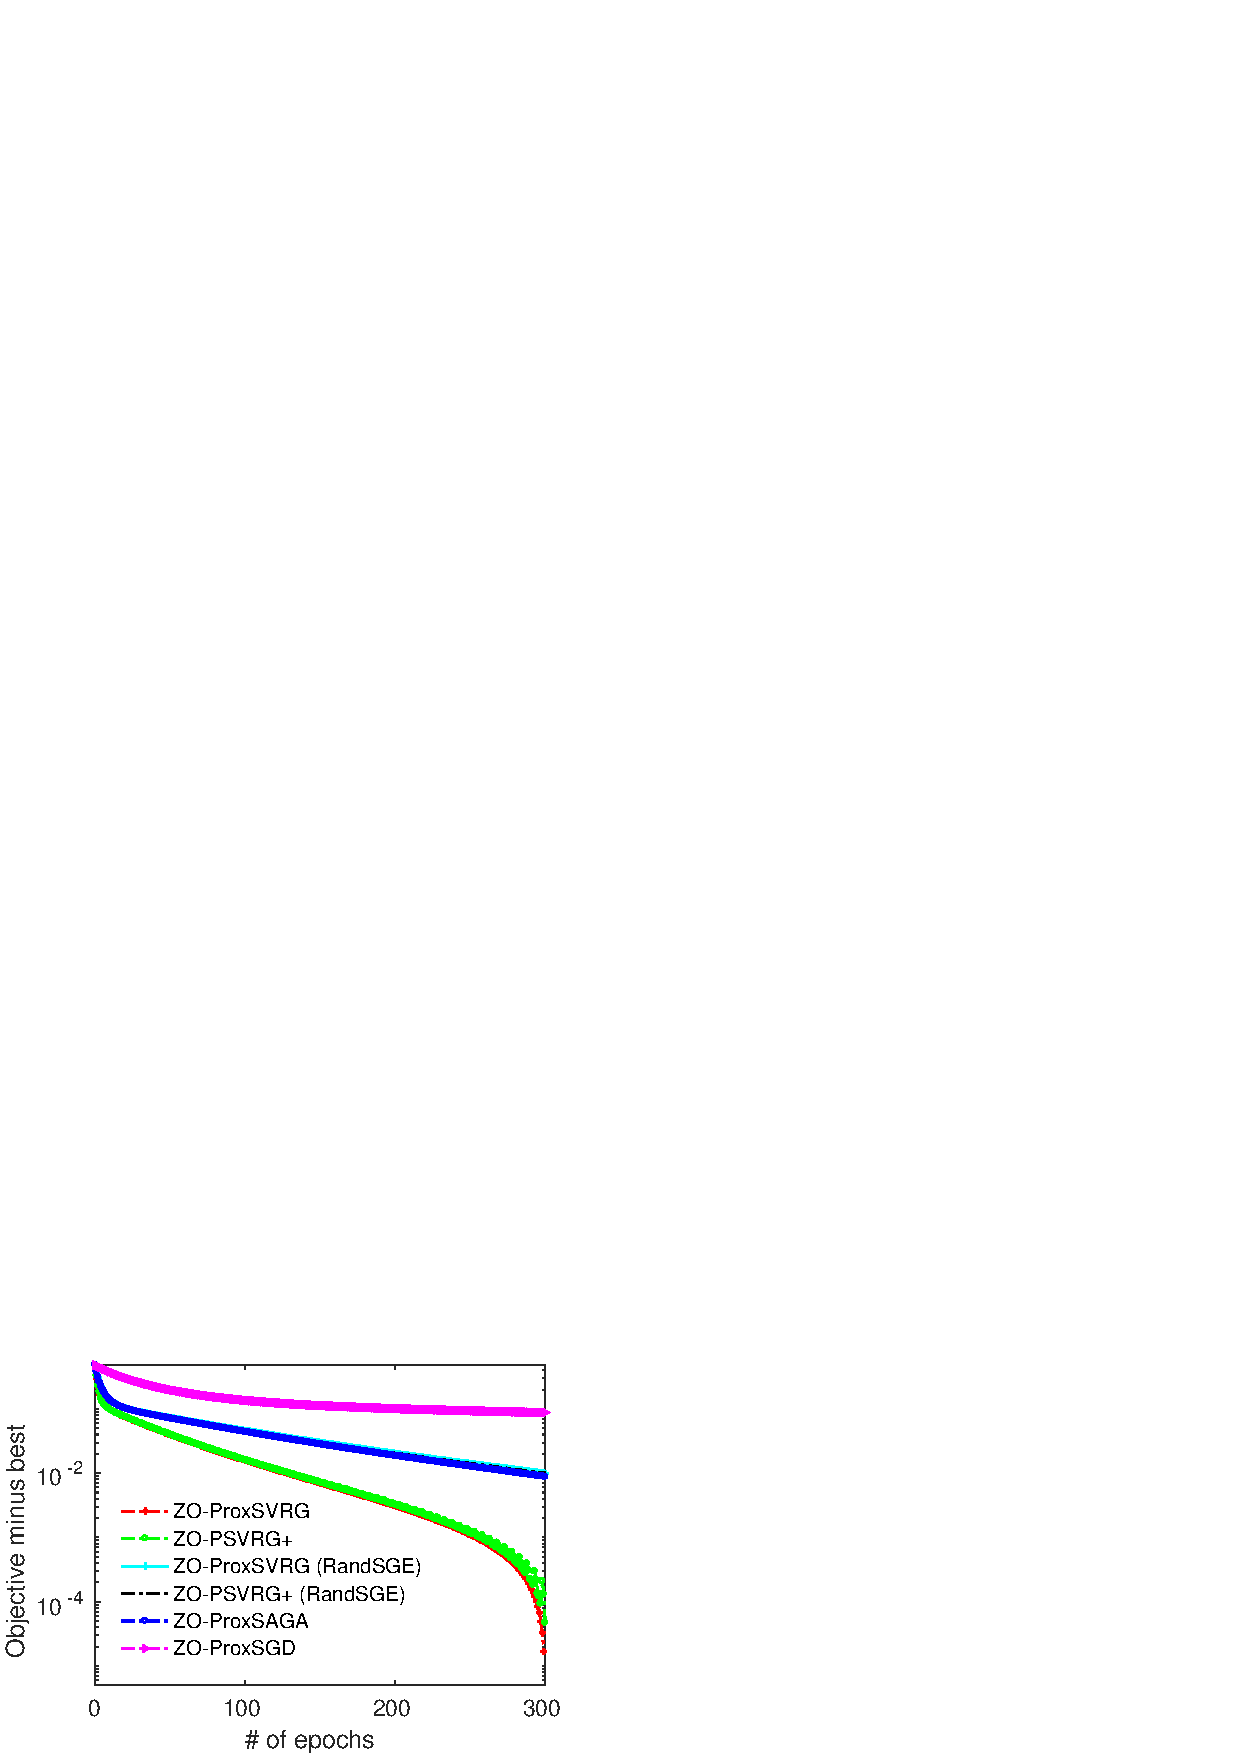
\includegraphics[width=0.23\linewidth]{ijcnn1b50k1.pdf}}%
\addtocounter{subfigure}{-4}
\subfloat{
\centering
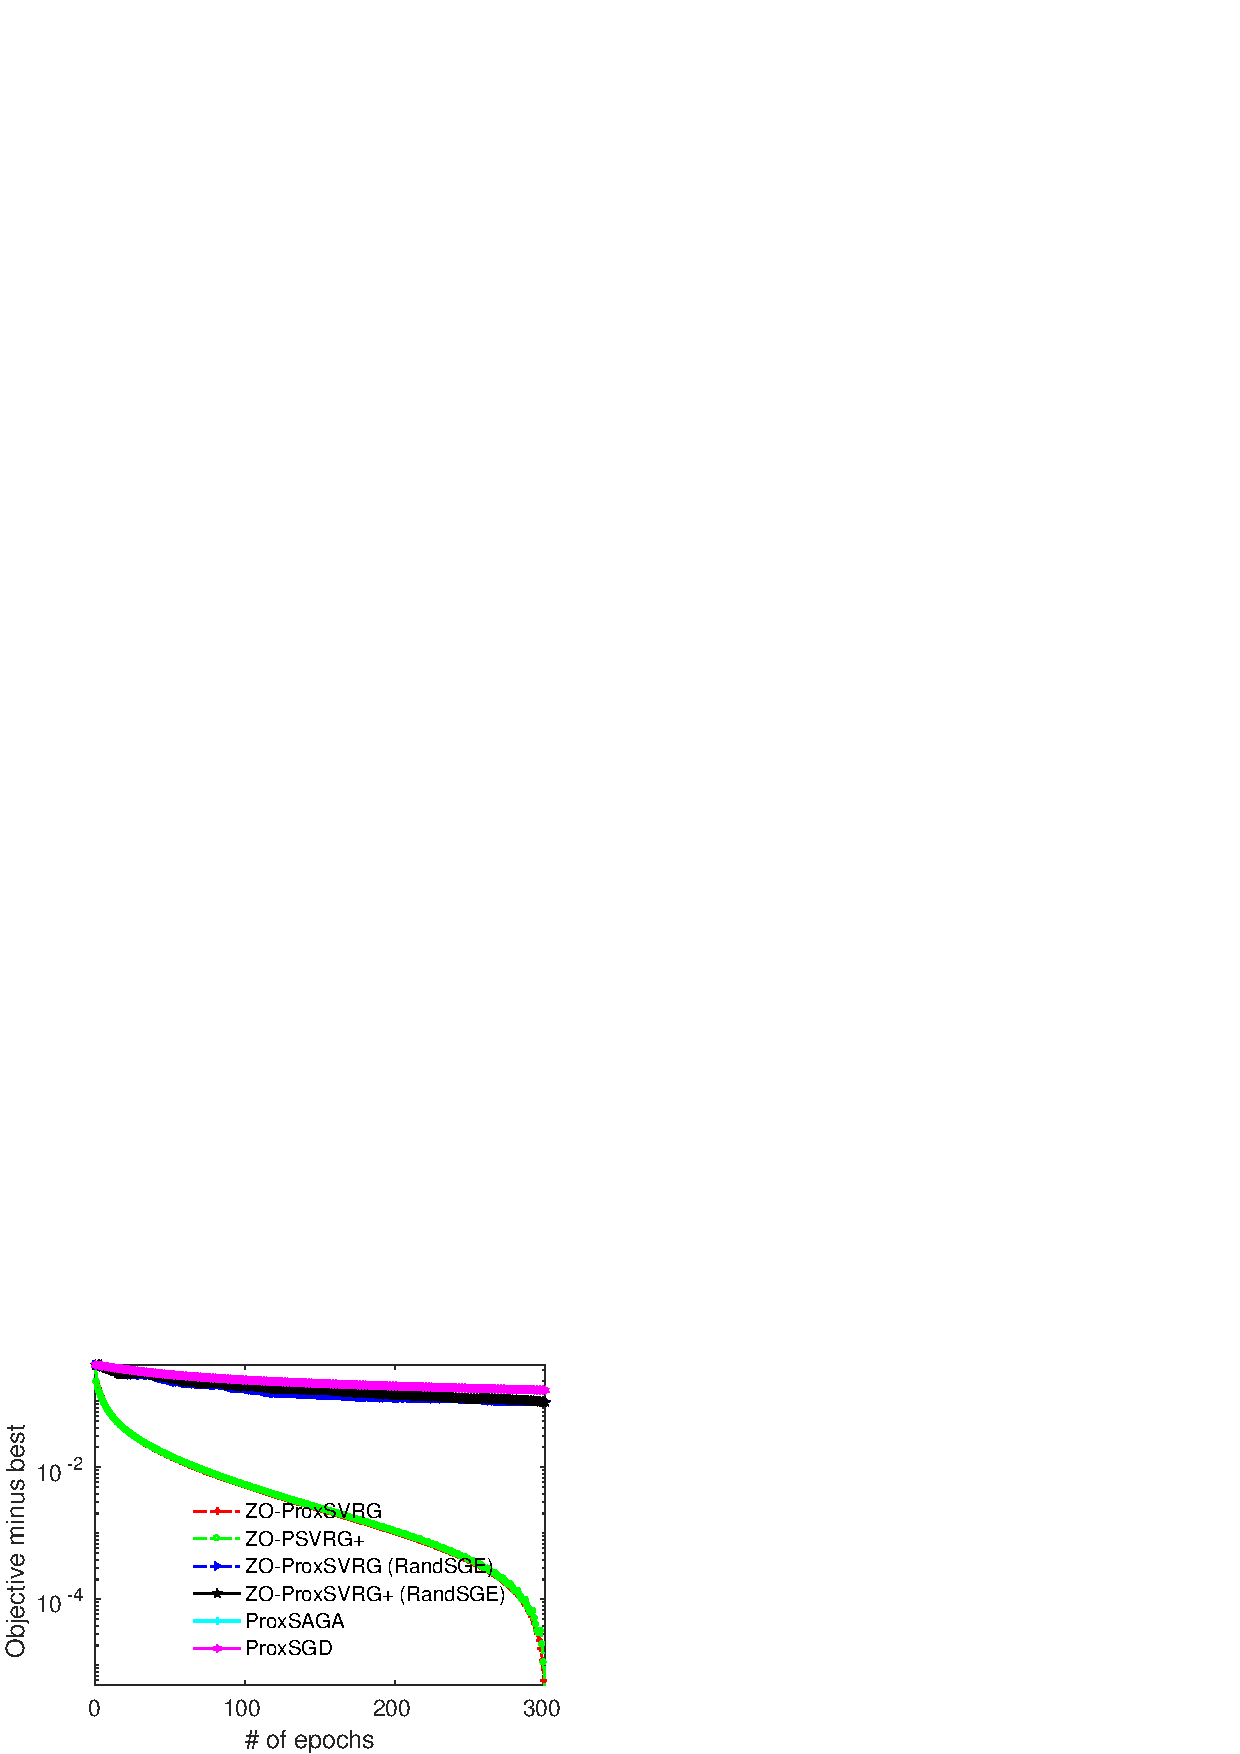
\includegraphics[width=0.23\linewidth]{adultb50k1.pdf}}%
\subfloat{
\centering
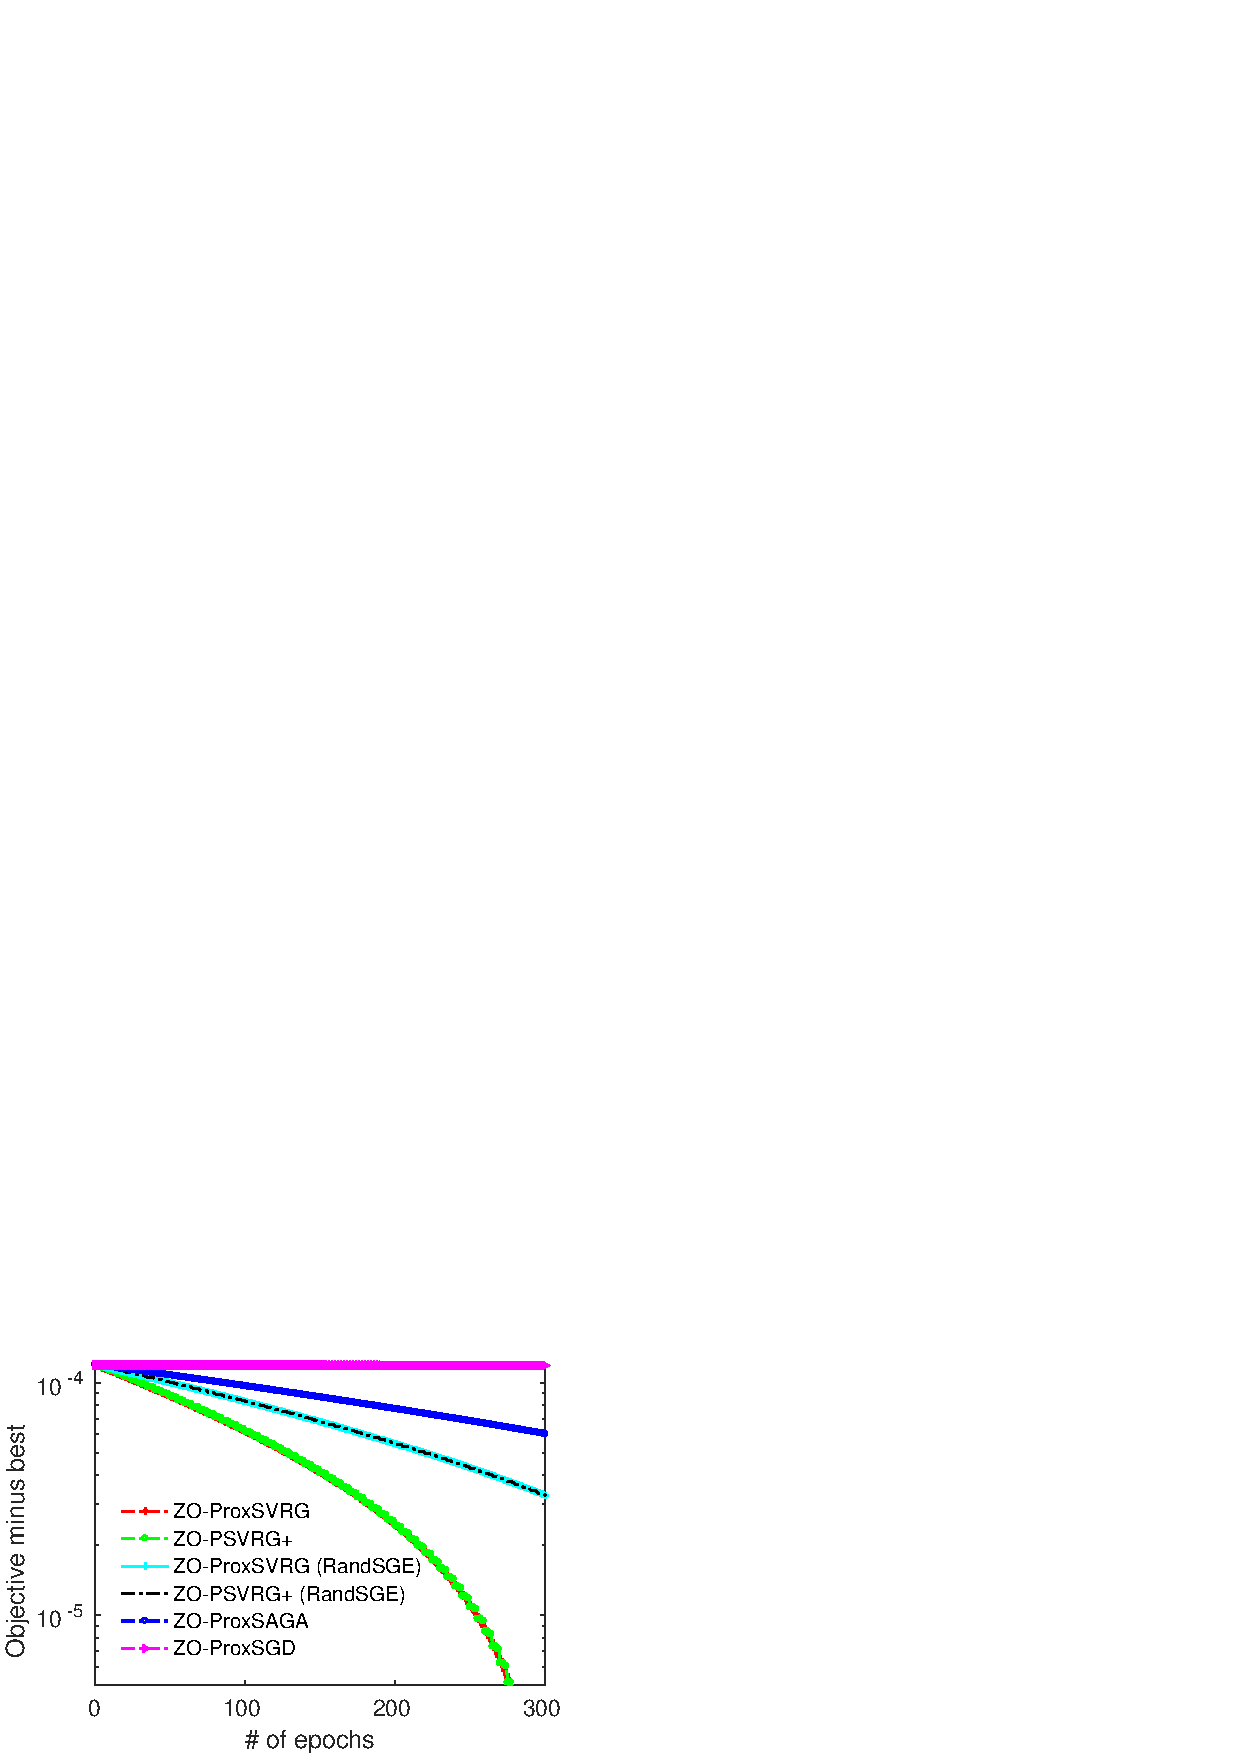
\includegraphics[width=0.23\linewidth]{w8ab50k1.pdf}}%
\subfloat{
\centering
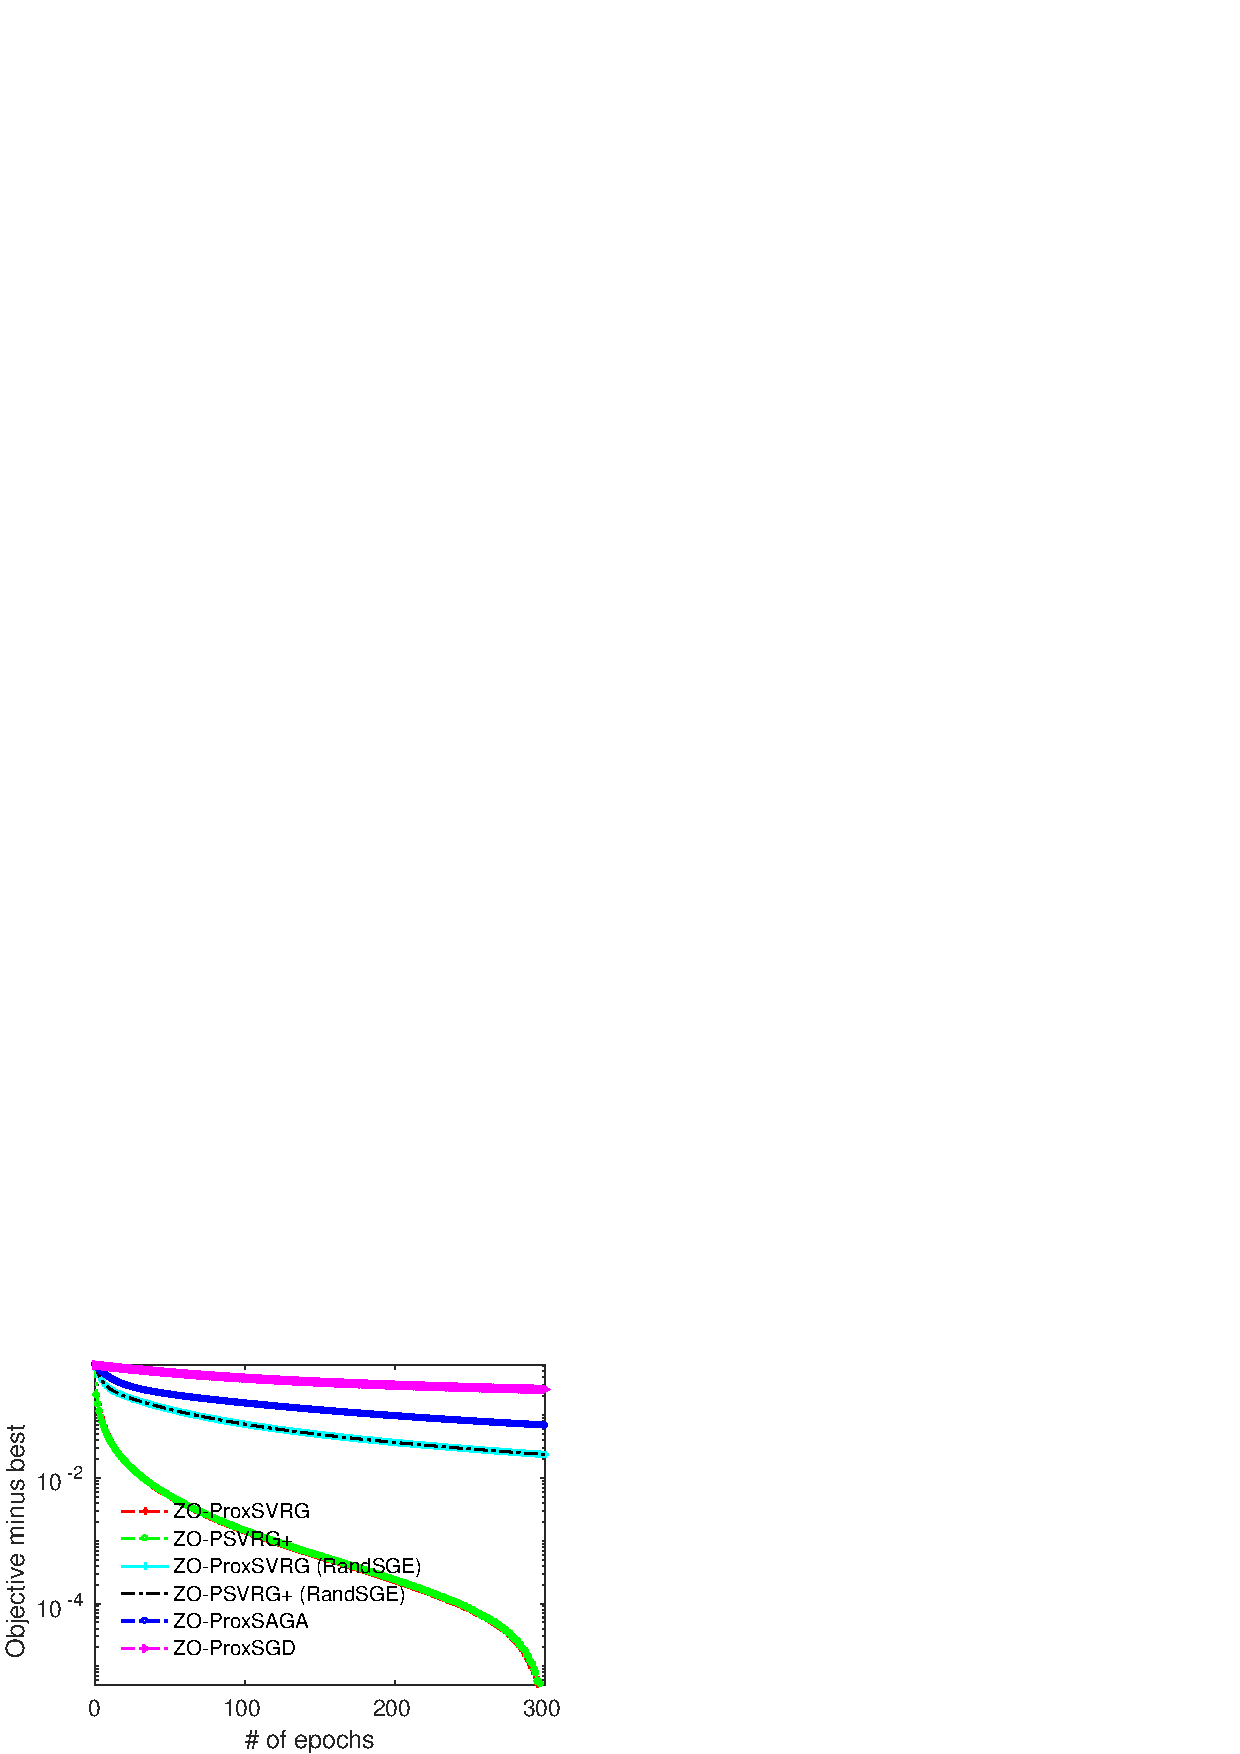
\includegraphics[width=0.23\linewidth]{mnistb50k1.pdf}}\\
\subfloat[ijcnn]{
\centering
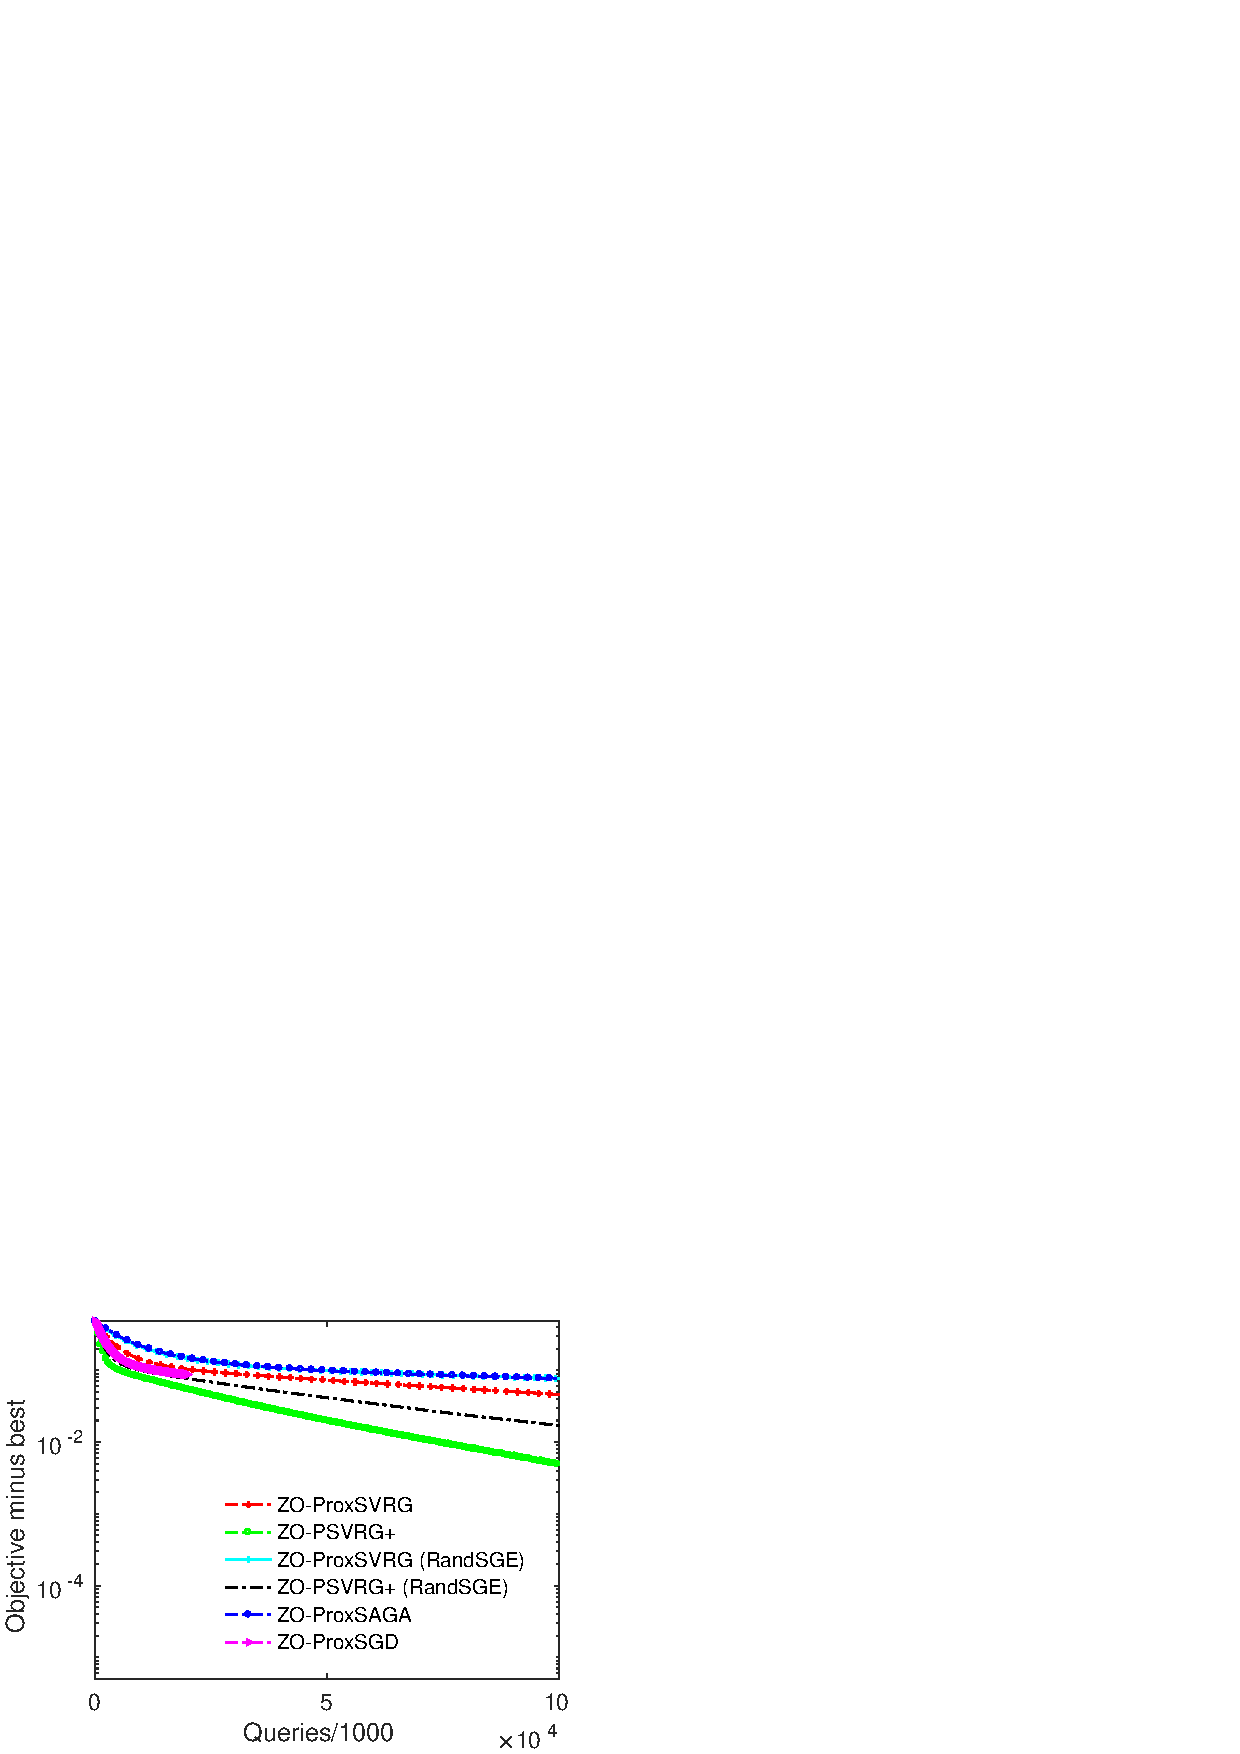
\includegraphics[width=0.23\linewidth]{ijcnn1b50k2.pdf}}%
\subfloat[comparison on covtype]{
\centering
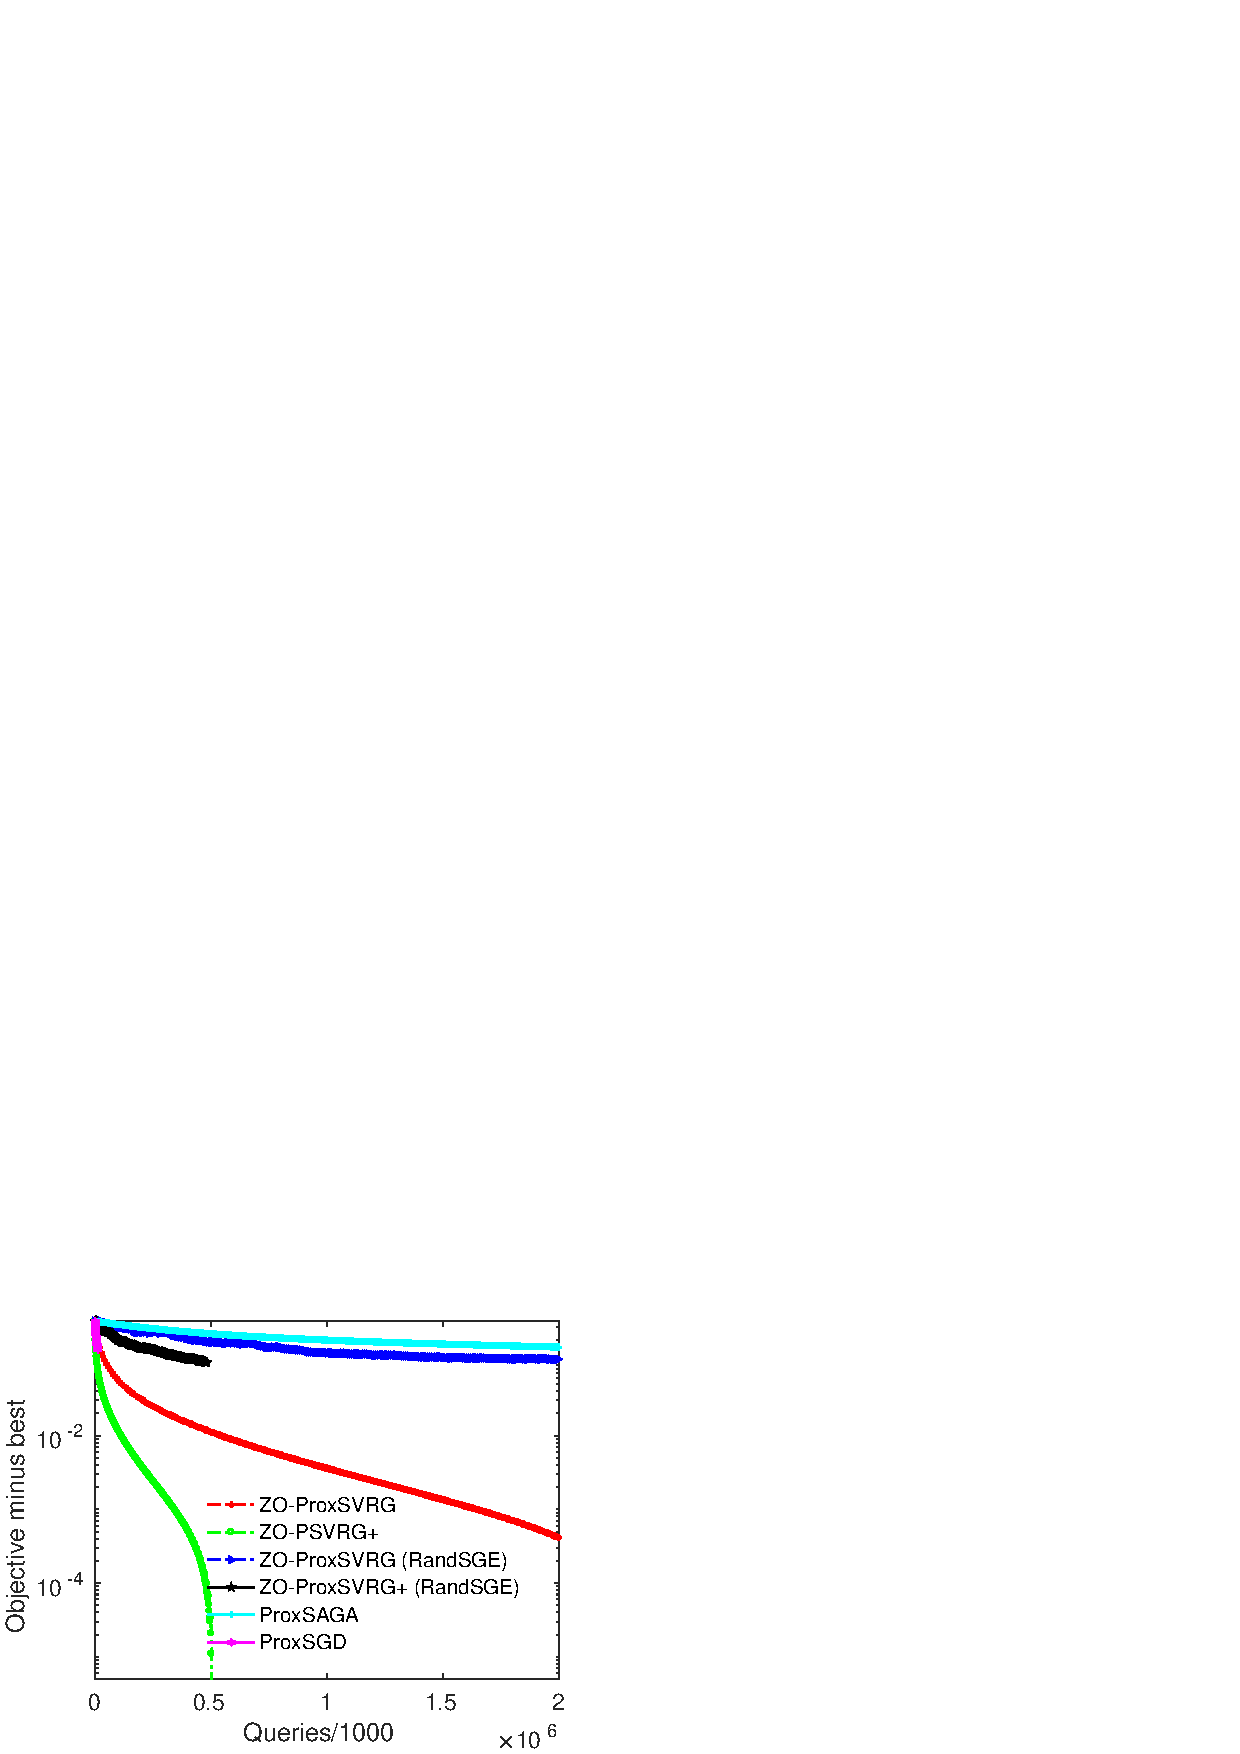
\includegraphics[width=0.23\linewidth]{adultb50k2.pdf}}%
\subfloat[w8a]{
\centering
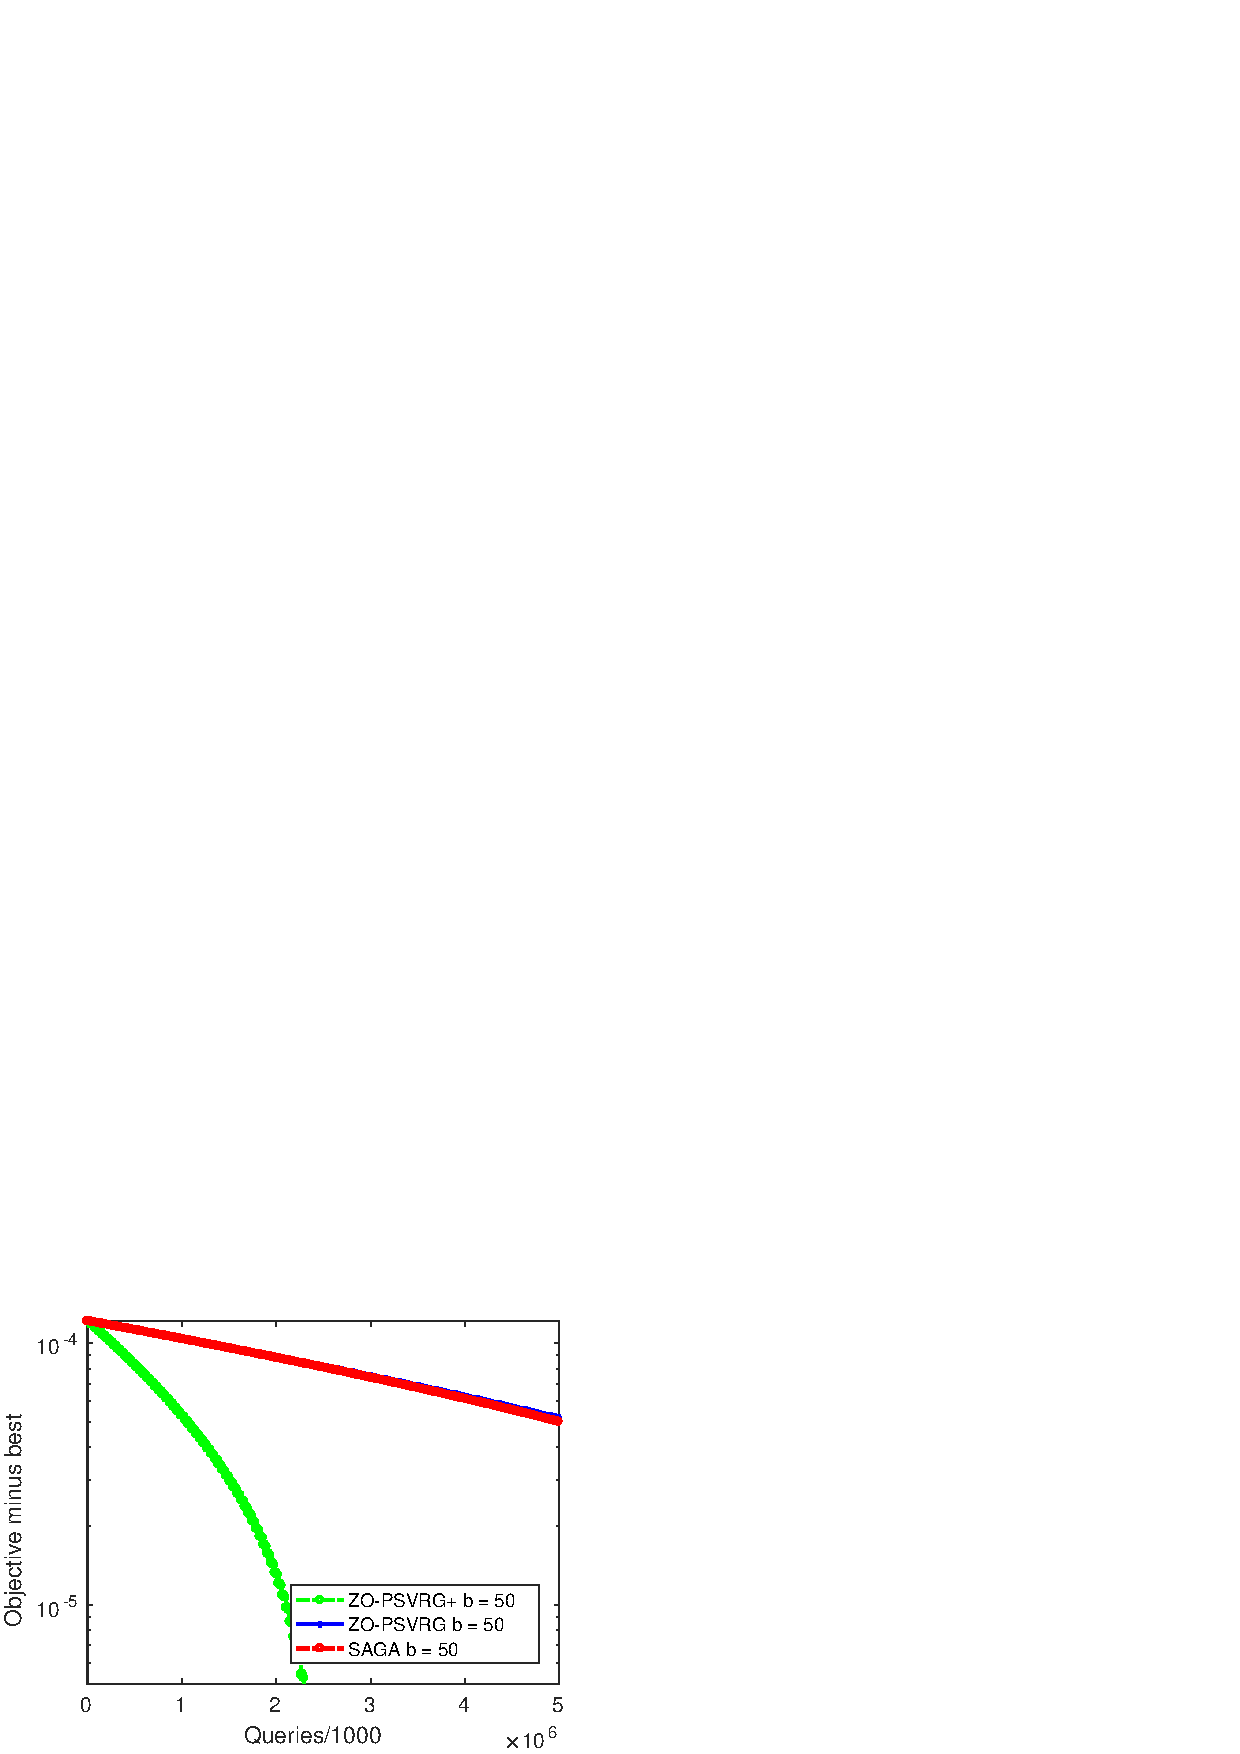
\includegraphics[width=0.23\linewidth]{w8ab50k2.pdf}}%
\subfloat[mnist]{
\centering
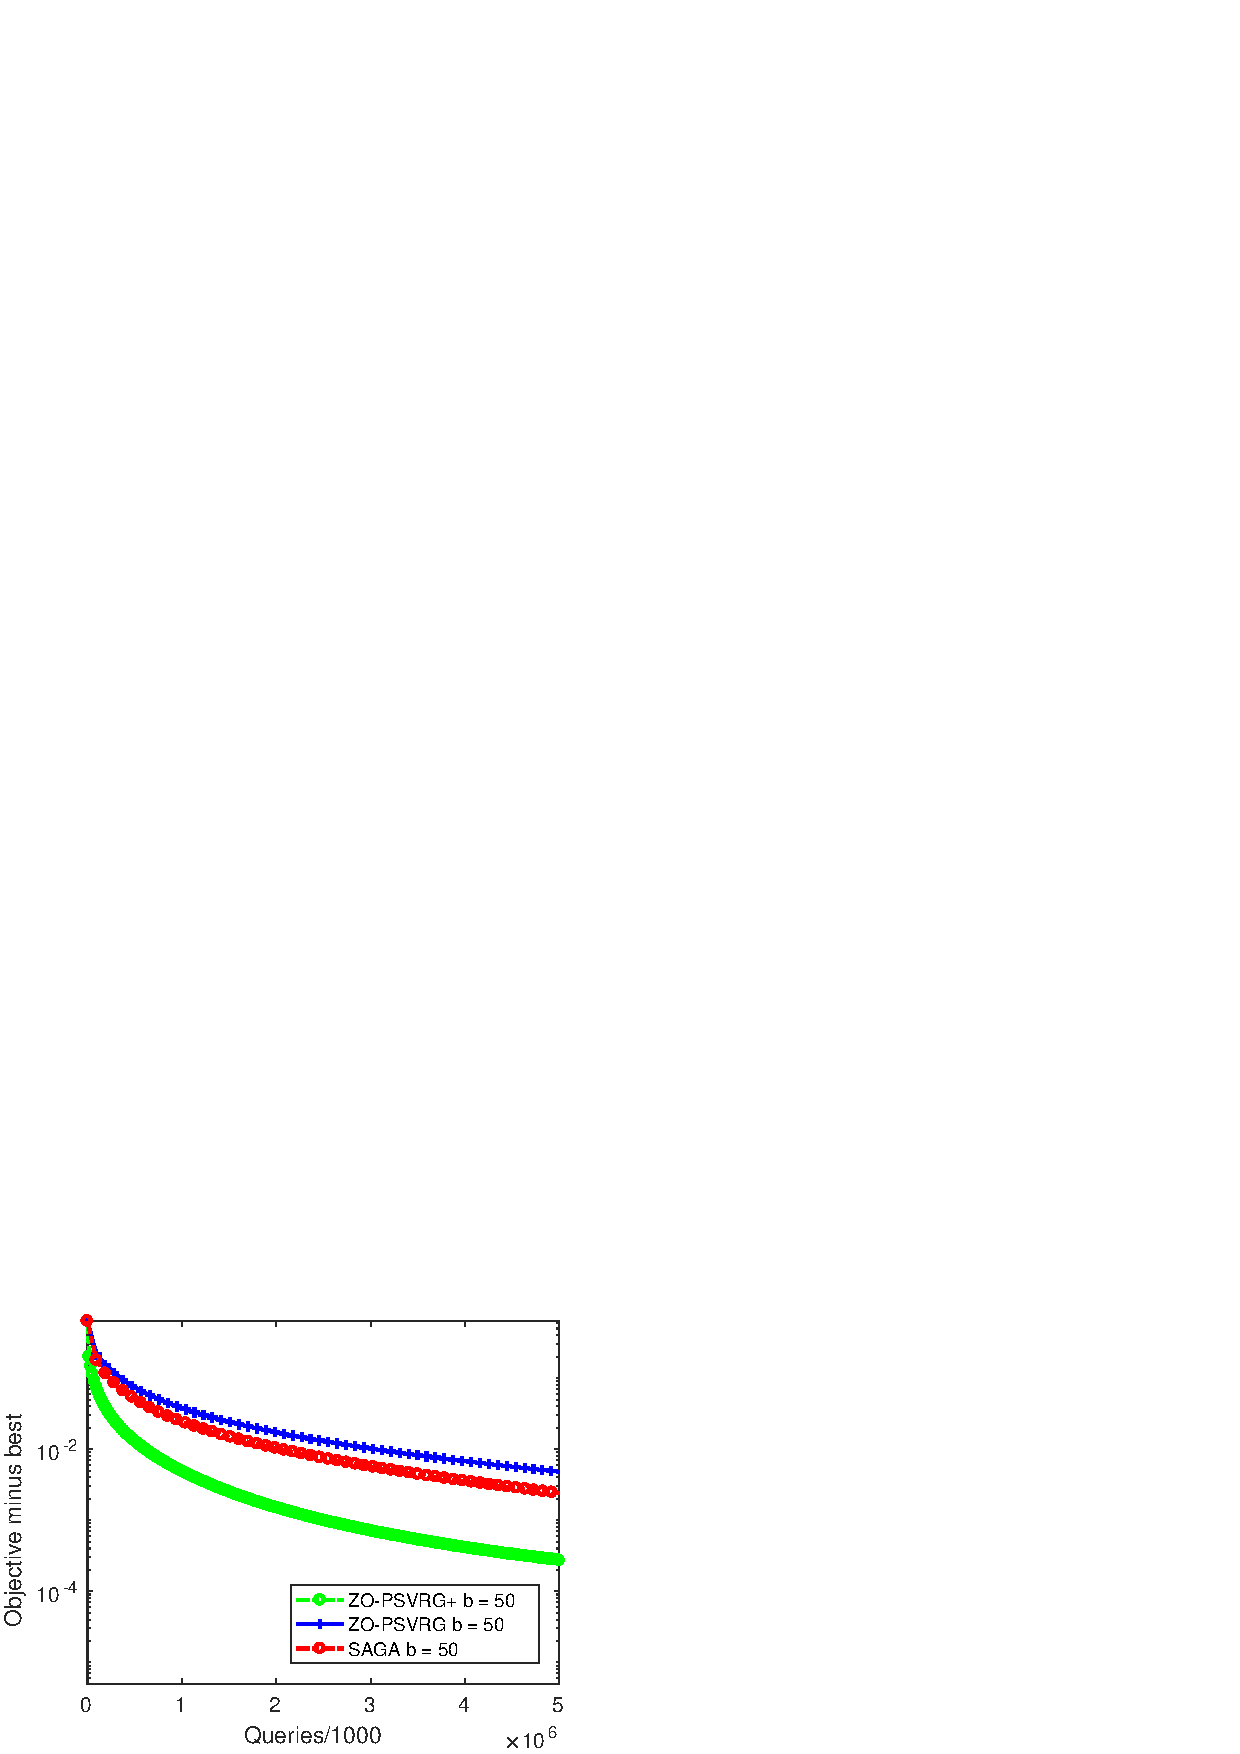
\includegraphics[width=0.23\linewidth]{mnistb50k2.pdf}}%
\setlength{\abovecaptionskip}{2pt}
\caption{Comparison of different zeroth-order algorithms for logistic regression loss residual $f(x) - f(x^*)$ versus the number of epochs (top) and ZO queries (bottom)}
\label{binary-fig}
\end{figure*}
In this section, we provide our experimental results. We compare the performance of
our ZO-PSVRG+ and ZO-PSPIDER+ with 1) ZO-ProxSVRG (based on our improved analysis), 2) ZO-ProxSAGA-Coord \cite{gu2018faster} and 3) ZO-ProxSGD \cite{ghadimi2016accelerated} over two empirical experiments: black-box binary classification and adversarial attacks for black-box deep neural networks (DNNs). We let ZO-ProxSGD denote RSPGF using CoordSGE \eqref{gradestcoord} for gradient estimation. We also let ZO-ProxSVRG and ZO-ProxSVRG (RandSGE) denote ZO-PSVRG+ and ZO-PSVRG+ (RandSGE) with $\mathcal{B} = n$, respectively. The learning rates are tuned in the experiments for competitive algorithms according to their convergence guarantees in Tables \ref{table-compare} and \ref{table-compare-spider}, and the results shown in this section are based on the best learning rate we obtained for each algorithm. More specifically, Tables \ref{table-compare} and \ref{table-compare-spider} show if the stepsize has to be dependent on the dimension $d$ for the convergence guarantee. We set stepsize $\eta$ and smoothing parameter $\mu$ for ZO-PSVRG+ and ZO-PSVRG+ (RandSGE) according to the convergence results that we obtained in the studied lemmas and theorems.
%$f_i(x) = \log(1+e^{-y_iz^T_i{x}})$

\subsection{Binary Classification}

In the first set of our experiments, we investigate the logistic regression loss function with $L_1$ and $L_2$ regularization for training the black-box binary classification problem. The problem can be described as the optimization problem \eqref{problem} with $f_i(x) = \frac{1}{1+e^{y_iz^T_i{x}}}$, $h(x) = \lambda_1\|{x}\|_1 + \frac{\lambda_2}{2}\|{x}\|^2$, where $z_i\in\R^d$ and $y_i$ is the corresponding label for each $i$. The $L_1$ and $L_2$ regularization weights $\lambda_1$ and $\lambda_2$ in all the experiments are set respectively to $10^{-4}$ and $10^{-6}$. We also set $\mathcal{B} = \lfloor{\frac{n}{5}}\rfloor$ for ZO-PSVRG+. We run our experiments on datasets from LIBSVM website{\footnote{https://www.csie.ntu.edu.tw/~cjlin/libsvmtools/datasets/binary.html}}, as listed in Table \ref{metadata}. The epoch size is chosen $m = 30$ over all the  experiments and the minibatch size $b$ is set to $50$. 
 
\begin{table}[htbp]
\begin{center}
\caption{Summary of training datasets.}
\begin{tabular}{ c|c|c } 
 \hline
 Datasets &  Data & Features \\ 
 \hline
  ijcnn & 49990 & 22 \\
  a9a & 32561 & 123 \\ 
 w8a & 64,700  & 300 \\ 
 mnist & 60000 & 784 \\
%  \hline
% SUSY & 5,000,000 & 18 &  88,938,127 \\
 %epsilon &  400,000 & 2,000 &  800,000,000 \\
 %kdd12 & 119,705,032 & 54,686,452 & 0 \\
 \hline
\end{tabular}
\label{metadata}
\end{center}
\end{table}

In Figure \ref{binary-fig} (top), we show the training loss versus the number of epochs (i.e., iterations divided by the
epoch length $m = 30$). Note that ZO-PSVRG+ is evaluated using mix gradient CoordSGE \eqref{gradestcoord} and mix gradient RandSGE \eqref{gradestrand}.
Results in Figure \ref{binary-fig} (bottom) compare the performance of ZO-PSVRG+ with the variants of ZO variance reduced stochastic gradient descent described earlier in Table \ref{table-compare} against the number of function queries. In these figures, ZO-PSVRG+  shows a faster convergence rate compared to ZO-PSVRG+ (RandSGE). Note that ZO-ProxSVRG based on
our improved analysis compared to \cite{huang2019faster} presents a better convergence than both ZO-ProxSAGA and  ZO-ProxSGD. On the other hand, the application of $\mathcal{B} = \lfloor{\frac{n}{5}}\rfloor$ in ZO-PSVRG+ significantly
improves ZO-ProxSVRG with respect to the number of ZO-queries (see Table \ref{table-compare}), leading to a non-dominant factor $O(I_{\{\mathcal{B} < n\}}/\mathcal{B})$ in the convergence rate of ZO-PSVRG+. In particular, ZO-PSVRG+ exhibits better performance in terms of the number of function queries than ZO-ProxSAGA using CoordSGE.  The degradation in the convergence of ZO-ProxSAGA is due to the requirement for small stepsizes $O(\frac{1}{d})$. Furthermore, the large number of function queries to construct
coordinate-wise gradient estimates significantly increases the number of SZO queries for ZO-ProxSVRG. On the other hand, ZO-ProxSGD consumes an extremely large number of iterations while exhibiting marginal convergence compared with variance-reduced algorithms. Thus, ZO-PSVRG+ and ZO-PSPIDER+ obtain the best trade-offs between the iteration and the function query complexity. The figure shows the convergence from ZO-PSPIDER+ marginally outperforms the one from ZO-PSVRG+.
\begin{figure*}[hbt!]
\subfloat[Loss vs iterations: $n = 10$]{
\centering
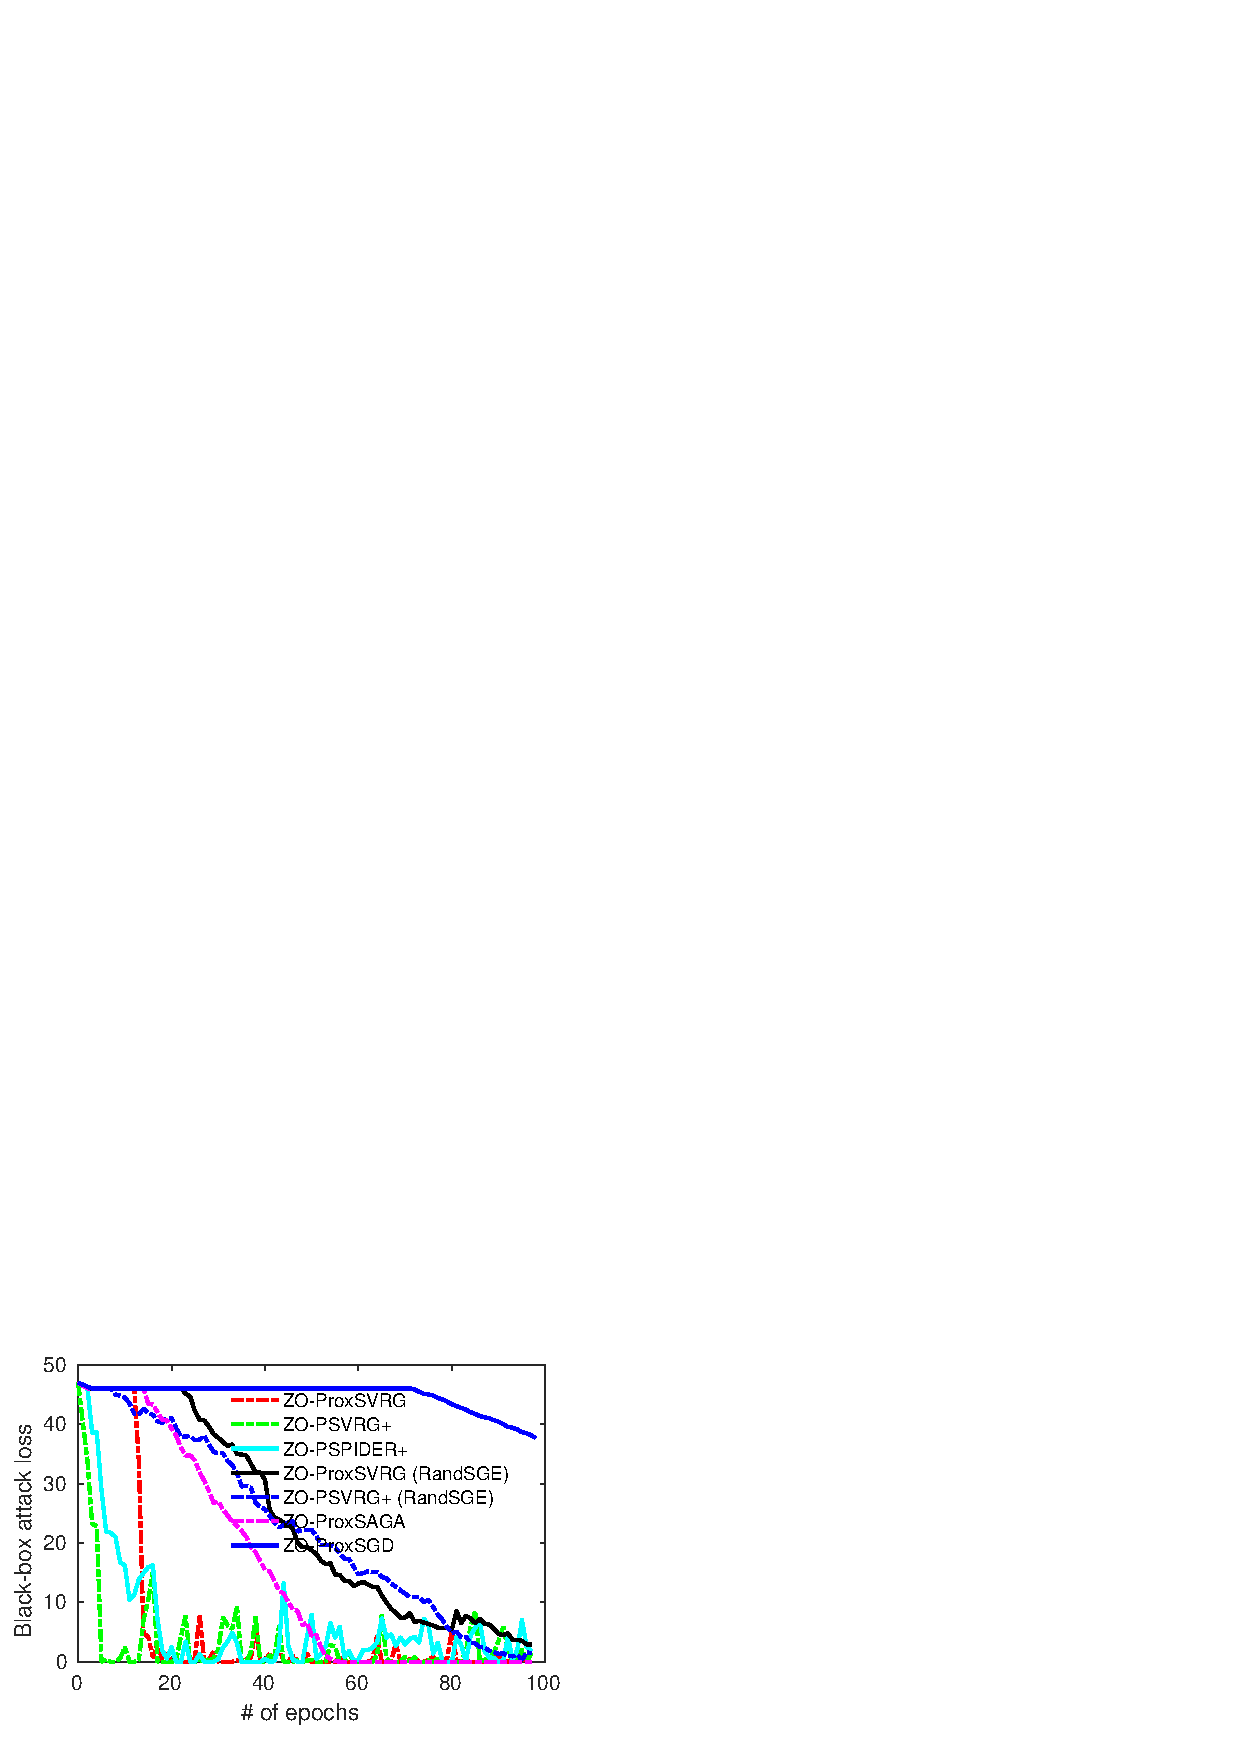
\includegraphics[width=0.44\linewidth]{figiter.pdf}}\hfill%
\subfloat[Loss vs queries: $n = 10$]{
\centering
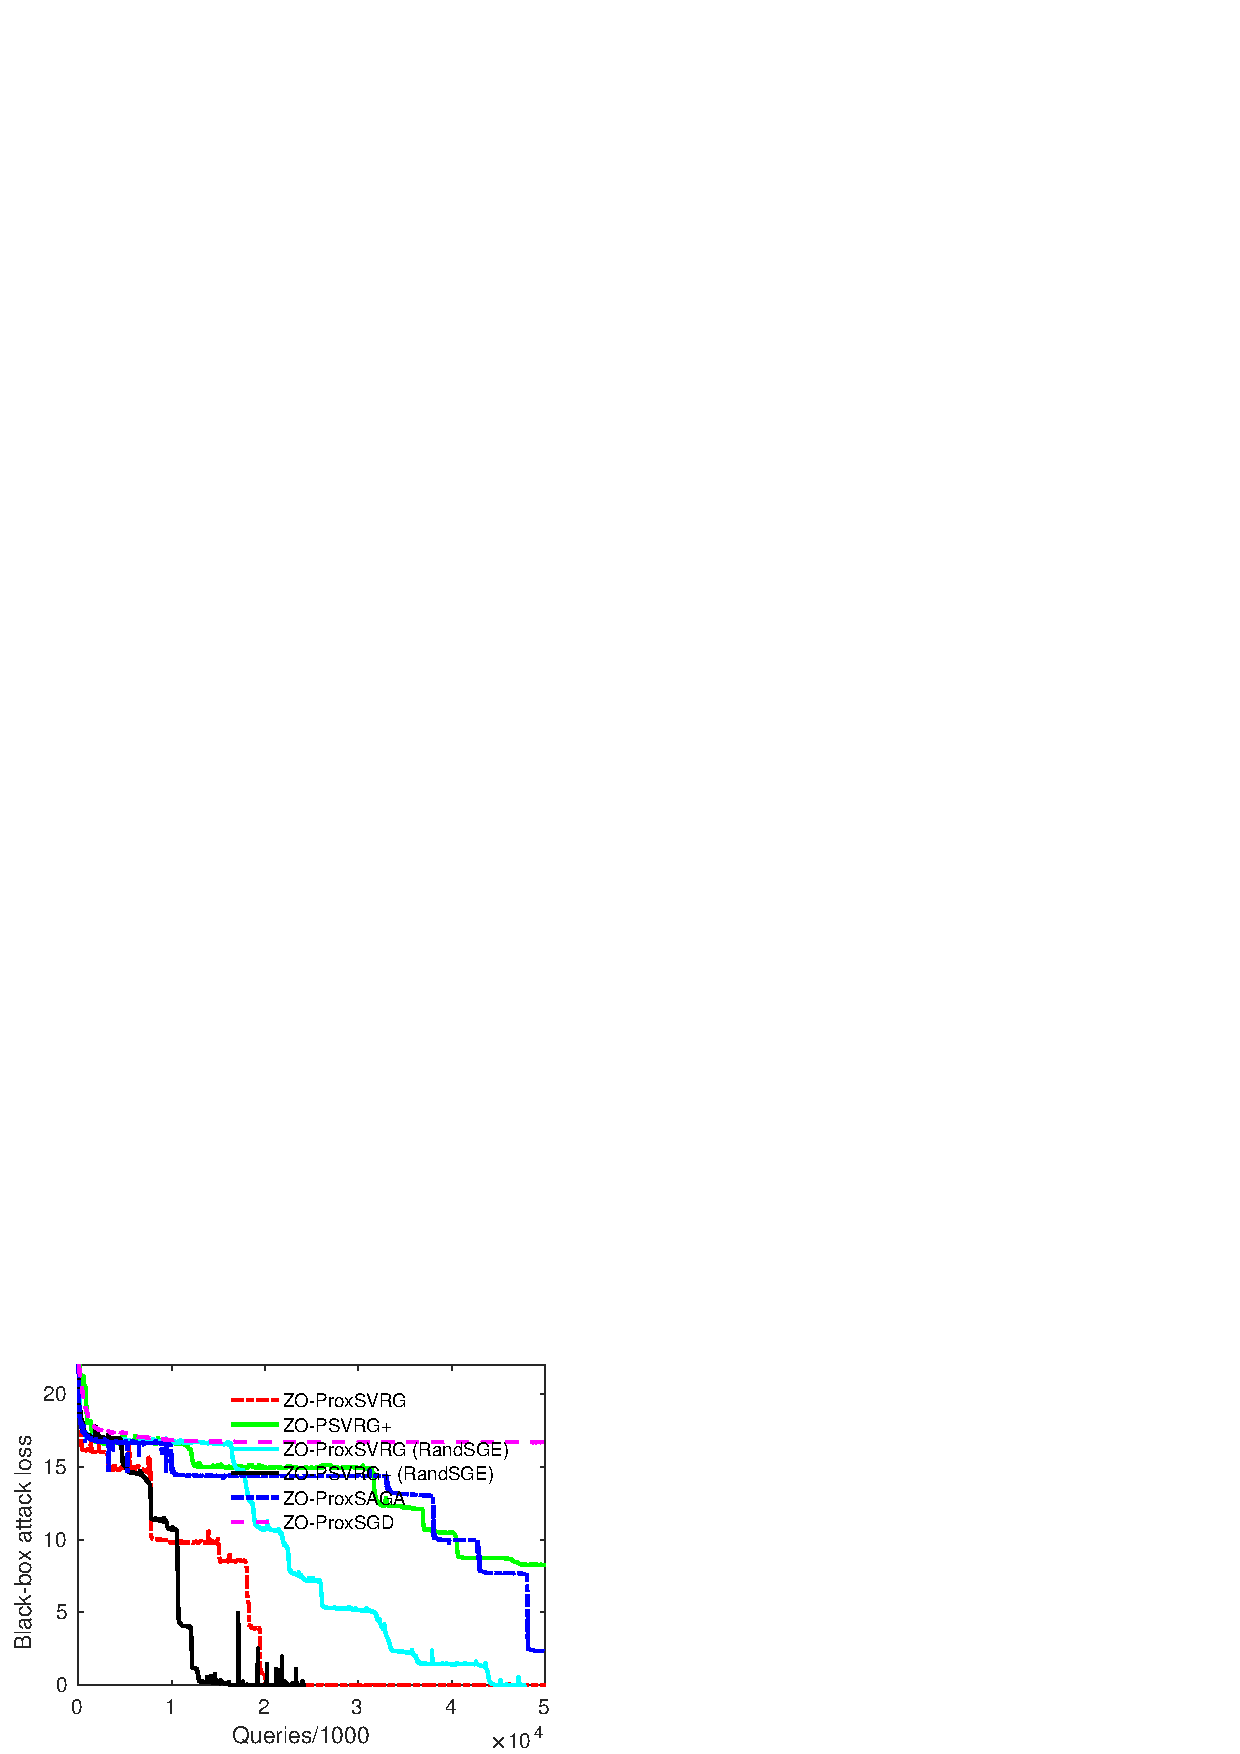
\includegraphics[width=0.42\linewidth]{figquery.pdf}}%
\setlength{\abovecaptionskip}{2pt}
\caption{Comparison of different zeroth-order algorithms for generating black-box adversarial examples from a black-box DNN over MNIST dataset}
\label{attack-fig}
\end{figure*}

\begin{figure*}[hbt!]
\subfloat[Loss vs iterations: $n = 10$]{
\centering
\includegraphics[width=0.44\linewidth]{figiter_cifar10.pdf}}\hfill%
\subfloat[Loss vs queries: $n = 10$]{
\centering
\includegraphics[width=0.42\linewidth]{figquery_cifar10.pdf}}%
\setlength{\abovecaptionskip}{2pt}
\caption{Comparison of different zeroth-order algorithms for generating black-box adversarial examples from a black-box DNN over CIFAR-10 dataset}
\label{attack-fig-cifar10}
\end{figure*}

\begin{figure*}[hbt!]
\subfloat{
\centering
\includegraphics[width=1.0\linewidth]{mnist.png}}%
\setlength{\abovecaptionskip}{2pt}
\caption{Images of universal perturbation $\delta := a_i^{adv} - a_i$ from different proximal ZO algorithms and the subsequent generated adversarial images for the class label ``1'' of the MNIST dataset. The left nine columns show the generated adversarial examples crafted by different ZO algorithms. The second last columns present a visualization for the universal perturbation $\delta$ for each ZO algorithm and the last column shows the $L_2$-norm of the generated universal perturbation ($\norm{\delta}$). The bottom of each subplot for adversarial attacks shows the label of the benign sample and the predicted label of the corresponding adversary (ground-truth label -> predicted label).}
\label{attack-perturbs-fig}
\end{figure*}



\subsection{Adversarial Attacks on Black-Box DNNs}
Adversarial 
examples in image classification are related to designing unperceptive perturbations such that they lead to misclassifying the target model when added to benign images. In the framework of zeroth-order attacks \cite{chen2017zoo,liu2018zeroth}, the model parameters are hidden, and gradient estimation is not feasible, while
the model output could be obtained. We formulate the task of generating a universal adversarial perturbation for $n$ natural images as a ZO optimization problem \eqref{problem}.
More precisely, we apply the zeroth-order algorithms to obtain a global adversarial perturbation $x\in\R^d$ that could mislead the classifier on samples $\{a_i \in \R^d, y_i\in\mathbb{N} \}_{i=1}^n$. This problem can be specified as the following elastic-net attacks to black-box DNNs problem:
\begin{align}
\min_{x\in\R^d} \frac{1}{n} \sum_{i=1}^n& \max\{F_{y_i}(a_i^{adv}) - \max_{j\neq y_i}F_j(a_i^{adv}),0\}\notag\\
& + c\norm{a_i^{adv} - a_i}^2 + \lambda_1 \norm{x}_{1} + \lambda_2 \norm{x}^{2}\label{mnist-attack-loss}
\end{align}
where $a_i^{adv} = 0.5\tanh(\tanh^{-1}(2a_i)+x)$ and $\lambda_1$ and $\lambda_2$ are nonnegative parameters to obtain consonance between attack success rate, distortion, and sparsity. Here $F(a) = \left[F_1(a),\ldots, F_K(a)\right]\in [0, 1]^K$ describes a trained deep neural network (DNN) for  K-class classification task, where $F_i(a)$ returns the prediction score of $i$-th class. The parameter $c$ in \eqref{mnist-attack-loss} compensate the rate of adversarial success and the distortion of adversarial examples. In our experiment, we set the regularization parameter  $c = 0.2$ and $\lambda_1 = \lambda_2  = 10^{-5}$ for MNIST dataset and $\lambda_1 = \lambda_2  = 0.1$ for CIFAR-10 dataset.

Our experiment setting is to generate universal black-box adversarial perturbation on $n = 10$ samples images from the same class over MNIST and CIFAR-10 datasets. We set the minibatch size to $b=5$. We select the batch size $\mathcal{B} = \lfloor{\frac{n}{2}}\rfloor$ for ZO-PSVRG+ and ZO-PSPIDER+.
Figures \ref{attack-fig} and \ref{attack-fig-cifar10} show
the performance of different ZO algorithms in this paper over MNIST and CIFAR-10 datasets, respectively. Figure \ref{attack-fig} shows that our two algorithms ZO-PSVRG+ (RandSGE) and ZO-ProxSVRG (under our improved analysis) provide better performance
both in convergence rate (iteration complexity) and function query complexity than ZO-ProxSGD
and ZO-ProxSAGA. The performance of ZO-PSVRG+ (CoordSGE) algorithm degrades due to a large number of function queries for CoordSGE and the variance inherited by $\mathcal{B} \neq n$. 
ZO-PSVRG+ (RandSGE) shows faster convergence in the initial optimization stage, and more importantly, has much lower function query complexity, which is largely
due to efficient ZO queries for computing mix gradient \eqref{zo-grad-fo-rand} and  the $O(\frac{1}{\sqrt{d}})$-level stepsize required by ZO-PSVRG+ (RandSGE). ZO-ProxSAGA and ZO-PSVRG+ (CoordSGE) exhibit relatively similar convergence behaviors. Furthermore, the convergence performance of ZO-ProxSGD is poor compared to the other algorithms due to not using variance-reduced acceleration techniques. Similar observations are found in Figure \ref{attack-fig-cifar10} for CIFAR-10 dataset where the results for ZO-PSVRG+ and ZO-PSPIDER+ outperform the competitors in terms of convergence rate and function queries.

We visualize the pattern of generated universal perturbations and eventually the adversarial examples for class label ``1'' in Figure \ref{attack-perturbs-fig} and in Figure \ref{attack-perturbs-cifar-fig} in the supplementary materials. Figure \ref{attack-perturbs-fig} shows that the ZO algorithms with CoordSGE produce structured perturbations whereas the adversarial distortion produced with RandSGE scheme is unstructured and presents irregular patterns. We also observe that the patterns of the crafted universal perturbation form ZO-PSVRG+ and ZO-PSPIDER+ identify the most distinctive image segments corresponding to the ground-truth label ``1''. In addition, while each proximal ZO algorithm produces universal adversarial perturbation leading to mostly successful black-box attacks (misclassified samples), our attacks yield the best trade-offs between the attack success rate and the amount of the produced universal distortion in $L_2$-norm.

\section{Conclusion}
In this paper, we developed a novel analysis for two zeroth-order variance-reduced proximal algorithms, ZO-PSVRG+ and ZO-PSPIDER+ with CoordSGE and RangSGE zeroth-order gradient estimation and bring the convergence analyses from all the studied algorithms into uniformity. Our convergence studies generalize and improve the analysis of several well-known convergence results, e.g., ZO-ProxSVRG and SPIDER-SZO. Compared with ZO-SVRG-Coord-Rand \cite{ji2019improved}, our analyses provide convergence guarantee and SZO calls complexity for all the minibatch sizes with large stepsizes. Moreover, for nonconvex functions under Polyak-Łojasiewicz condition, we prove that ZO-PSVRG+ and ZO-PSPIDER+ obtain a global linear convergence rate for a wide range of minibatch sizes without restart. The empirical results demonstrate the effectiveness of our novel approaches. As a byproduct, our analysis provides the first step to lead the convergence studies of variance-reduced methods into compatible analyses which can be applied to other variance-reduced gradient-free approaches.\newpage
%\bibliographystyle{abbrv}
%references
\noindent\textbf{Funding} Not applicable.\\
\textbf{Availability of data and material} Not applicable.\\
\textbf{Declarations}\\
\textbf{Conflict of interest} Not applicable.\\
\textbf{Code availability} Available.\\
\textbf{Additional declarations} Not applicable.\\
\textbf{Ethics approval} Not applicable.\\
\textbf{Consent to participate} Not applicable.\\
\textbf{Consent for publication} Not applicable
\bibliography{GTA}
\onecolumn % <==========================================================
\renewcommand\theequation{A-\arabic{equation}}
\renewcommand{\theequation}{S\arabic{equation}}
\setcounter{equation}{0}
\setcounter{figure}{0}
\setcounter{table}{0}
\setcounter{page}{1}
\begin{center}
\textbf{\large Supplemental Materials}
\end{center}
In this section, we present the complete proofs of the above lemmas and theorems.

The following two lemmas are similar to \cite[Lemma 1, Lemma 2]{reddi2016proximal}, \cite[Lemma 1, Proposition 1]{ghadimi2013stochastic} and \cite[Lemma 1, Lemma 2]{li2018simple}.
We added the proof for these lemmas for completeness. 
\begin{lemma}\label{lemma1}
For a given $x \in \R^d$, let $\overline{x} = \Po_{\eta h}(x-\eta v)$, then we have for all $w\in \R^d$
\begin{equation}\label{eq10}
\begin{split}
F(\overline{x}) \leq F(w) &+ \Iprod{\nabla f(x)-v}{\overline{x}-w}-\frac{1}{\eta} \Iprod{\overline{x}-x}{\overline{x}-w}\\
&+\frac{L}{2}\norm{\overline{x}-x}^2+\frac{L}{2}\norm{w-x}^2 
\end{split}
\end{equation}
\end{lemma}
\begin{proof}
First, we recall the proximal operator 
\begin{equation}\label{eq11}
\Po_{\eta h}(x-\eta v) := \text{arg}\,\,\min_{y\in\R^d}\left(h(y)+\frac{1}{2\eta}\norm{y-x}^2+\Iprod{v}{y}\right)
\end{equation}
For the nonsmooth function $h(x)$, for all $w\in\R^d$ we have 
\begin{equation}\label{eq12}
\begin{split}
h(\overline{x}) &\leq h(w) + \Iprod{p}{\overline{x}-w}\\
&= h(w) - \Iprod{v+\frac{1}{\eta}(\overline{x}-x)}{\overline{x}-w}
\end{split}
\end{equation}
where $p\in \partial h(\overline{x})$ such that $p+\frac{1}{\eta}(\overline{x}-x)+v = 0$ according to the optimality condition of \eqref{eq11}, and \eqref{eq12} due to the convexity of $h$. In addition, since since $f(x)$ is $L$-Lipschitz continuous, we have
\begin{equation}\label{eq14}
f(\overline{x}) \leq f(x)+\Iprod{\nabla f(x)}{\overline{x}-x}+\frac{L}{2}\norm{\overline{x}-x}^2
\end{equation}
and
\begin{equation}\label{eq15}
f(x) \leq f(w)+\Iprod{\nabla f(x)}{x-w}+\frac{L}{2}\norm{w-x}^2
\end{equation}
 This lemma is obtained by adding \eqref{eq12}, \eqref{eq14}, \eqref{eq15}, and using $F(x) = f(x)+h(x)$. 
\end{proof}
\begin{lemma}\label{lemm-est-grad}
Let  $x_{t}^s= \Po_{\eta h}(x_{t-1}^s - \eta \hat{v}_{t-1}^s)$ and $\overline{x}_{t}^s$ be the proximal projection using full true gradient, i.e., $\overline{x}_{t}^s= \Po_{\eta h}(x_{t-1}^s - \eta \nabla f(x_{t-1}^s))$. Then the following inequality holds
\[
\Iprod{\nabla f(x_{t-1}^s) -\hat{v}_{t-1}^s}{x_t^s -\overline{x}_t^s} \leq \eta\norm{\nabla f(x_{t-1}^s)-\hat{v}_{t-1}^s}^2
\]
\end{lemma}
\begin{proof}
Based on inequality \eqref{eq12} we obtain
\begin{align}
h(x_t^s)&\leq h(\overline{x}_t^s) - \Iprod{\hat{v}_{t-1}^s+\frac{1}{\eta}(x_t^s-x_{t-1}^s)}{x_t^s-\overline{x}_t^s}\label{lemm-est-grad-1}
\end{align}
\begin{align}
h(\overline{x}_t^s)&\leq h({x}_t^s) - \Iprod{\nabla f(x_{t-1}^s)+\frac{1}{\eta}(\overline{x}_t^s-x_{t-1}^s)}{\overline{x}_t^s-x_t^s}\label{lemm-est-grad-2}
\end{align}
By summing \eqref{lemm-est-grad-1} and \eqref{lemm-est-grad-2}, we have 
\begin{align}
\frac{1}{\eta}\Iprod{x_t^s -\overline{x}_t^s}{x_t^s -\overline{x}_t^s} &\leq \Iprod{\nabla f(x_{t-1}^s) -\hat{v}_{t-1}^s}{x_t^s -\overline{x}_t^s}\notag\\
\frac{1}{\eta}\norm{x_t^s -\overline{x}_t^s}^2 &\leq \norm{\nabla f(x_{t-1}^s) -\hat{v}_{t-1}^s}\norm{x_t^s -\overline{x}_t^s}\label{lemm-est-grad-3}
\end{align}
where \eqref{lemm-est-grad-3} holds by Cauchy-Schwarz inequality. 
Thus, we obtain
\begin{align}
\norm{x_t^s -\overline{x}_t^s} &\leq \eta\norm{\nabla f(x_{t-1}^s) -\hat{v}_{t-1}^s}\label{lemm-est-grad-4}
\end{align}
Now the proof is complete using Cauchy-Schwarz inequality and \eqref{lemm-est-grad-4}.
\end{proof}
Below, we start by deriving an upper bound for the variance of estimated gradient $\hat{v}_{t-1}^s$ based on CoordSGE. 
\begin{lemma}\label{var-estimate-lem}
Given the mix gradient estimation $\hat{v}_{t-1}^s = \frac{1}{b} \sum_{i\in I_b}\left(\hat{\nabla} f_{i}(x_{t-1}^s)-\hat{\nabla} f_{i}(\tilde{x}^{s-1})\right)+\hat{g}^s$ with $\hat{g}^s = \frac{1}{\mathcal{B}} \sum_{j\in I_{\mathcal{B}}} \hat{\nabla} f_j (\tilde{x}^{s-1})$, the following inequality holds. 
\begin{align}
\E&\left[\eta\norm{\nabla f(x_{t-1}^s)-{\hat{v}_{t-1}^s}}^2\right] \leq  \frac{6\eta L^2}{b}\E\left[\norm{x_{t-1}^s-\tilde{x}^{s-1}}^2\right]\notag\\
&+ 2\frac{I(\mathcal{B} < n)\eta \sigma ^2}{\mathcal{B}}+\eta \frac{7 L^2 d^2 \mu^2}{2}
\end{align}
where $I(A) = 1$ if the scenario $A$ occurs and $0$ otherwise.
\end{lemma}
Lemma \ref{var-estimate-lem} provides an upper bound for the variance of $\hat{v}_{t-1}^s$.  We will show later that both points $x_{t-1}^s$ and $\tilde{x}^{s-1}$ will converge to the same stationary point.  This results in reducing the variance of stochastic gradient, however, the variance is not totally diminished due to the zeroth-order gradient estimation and the variance of the gradient over batch.

\begin{proof}
We have
\begin{align}
  \E&\left[\eta\norm{\nabla f(x_{t-1}^s)-{\hat{v}_{t-1}^s}}^2\right]\notag\\
   =&\E\left[\eta\norm{\frac{1}{b}\sum_{i\in I_b}\left(\hat{\nabla} f_i(x_{t-1}^s)-\hat{\nabla} f_i(\tilde{x}^{s-1})\right) - \left(\nabla f(x_{t-1}^s)-\hat{g}^s\right)}^2\right]\notag\\
   =&\E\left[\eta\norm{\frac{1}{b}\sum_{i\in I_b}\left(\hat{\nabla} f_i(x_{t-1}^s)-\hat{\nabla} f_i(\tilde{x}^{s-1})\right) - \left(\nabla f(x_{t-1}^s)-\frac{1}{\mathcal{B}}\sum_{j\in I_{\mathcal{B}}}\hat{\nabla} f_j(\tilde{x}^{s-1})\right)}^2\right]\notag\\
   =&\notag\E\left[\eta\norm{\frac{1}{b}\sum_{i\in I_b}\left(\hat{\nabla} f_i(x_{t-1}^s)-\hat{\nabla} f_i(\tilde{x}^{s-1})\right) - \left(\nabla f(x_{t-1}^s) - \hat{\nabla} f(\tilde{x}^{s-1}) \right)+ \left(\frac{1}{\mathcal{B}}\sum_{j\in I_{\mathcal{B}}}\hat{\nabla} f_j(\tilde{x}^{s-1}) - \hat{\nabla} f(\tilde{x}^{s-1})\right)}^2\right]\\
   =&\notag\eta\E\left[\norm{\frac{1}{b}\sum_{i\in I_b}\left(\left(\hat{\nabla} f_i(x_{t-1}^s)-\hat{\nabla} f_i(\tilde{x}^{s-1})\right) - \left(\nabla f(x_{t-1}^s) - \hat{\nabla} f(\tilde{x}^{s-1}) \right)\right)+ \frac{1}{\mathcal{B}}\sum_{j\in I_{\mathcal{B}}}\left(\hat{\nabla} f_j(\tilde{x}^{s-1}) - \hat{\nabla} f(\tilde{x}^{s-1})\right)}^2\right]\\
   \leq &\notag2\eta\E\left[\norm{\frac{1}{b}\sum_{i\in I_b}\left(\left(\hat{\nabla} f_i(x_{t-1}^s)-\hat{\nabla} f_i(\tilde{x}^{s-1})\right) - \left(\hat{\nabla} f(x_{t-1}^s) - \hat{\nabla} f(\tilde{x}^{s-1}) \right)\right)+ \frac{1}{\mathcal{B}}\sum_{j\in I_{\mathcal{B}}}\left(\hat{\nabla} f_j(\tilde{x}^{s-1}) - \hat{\nabla} f(\tilde{x}^{s-1})\right)}^2\right]\\
   &\,\, + 2\eta \E \norm{\hat{\nabla} f(x_{t-1}^s)-\nabla f(x_{t-1}^s)}^2\label{var-estimate-lem-1}\\
    = &\notag 2 \eta\E\left[\norm{\frac{1}{b}\sum_{i\in I_b}\left(\left(\hat{\nabla} f_i(x_{t-1}^s)-\hat{\nabla} f_i(\tilde{x}^{s-1})\right) - \left(\hat{\nabla} f(x_{t-1}^s) - \hat{\nabla} f(\tilde{x}^{s-1}) \right)\right)}^2\right]\\
   &\,\, +2 \eta \E \left[ \norm{\frac{1}{\mathcal{B}}\sum_{j\in I_{\mathcal{B}}}\left(\hat{\nabla} f_j(\tilde{x}^{s-1}) - \hat{\nabla} f(\tilde{x}^{s-1})\right)}^2\right]+ 2\eta \E \norm{\hat{\nabla} f(x_{t-1}^s)-\nabla f(x_{t-1}^s)}^2\label{var-estimate-lem-2}\\
   = &\notag\frac{2\eta}{b^2}\E\left[\sum_{i\in I_b}\norm{\left(\left(\hat{\nabla} f_i(x_{t-1}^s)-\hat{\nabla} f_i(\tilde{x}^{s-1})\right) - \left({\hat{\nabla}} f(x_{t-1}^s) - \hat{\nabla} f(\tilde{x}^{s-1}) \right)\right)}^2\right]\\
   &\,\, \label{var-estimate-lem-3}+ 2\eta \E \left[ \norm{\frac{1}{\mathcal{B}}\sum_{j\in I_{\mathcal{B}}}\left(\hat{\nabla} f_j(\tilde{x}^{s-1}) - \hat{\nabla} f(\tilde{x}^{s-1})\right)}^2\right]+2\eta \E \norm{\hat{\nabla} f(x_{t-1}^s)-\nabla f(x_{t-1}^s)}^2\\
   \leq &\notag\frac{2\eta}{b^2}\E\left[\sum_{i\in I_b}\norm{\hat{\nabla} f_i(x_{t-1}^s)-\hat{\nabla} f_i(\tilde{x}^{s-1}) }^2\right]\\
   &\,\, \label{var-estimate-lem-3p}+ 2\eta \E \left[ \norm{\frac{1}{\mathcal{B}}\sum_{j\in I_{\mathcal{B}}}\left(\hat{\nabla} f_j(\tilde{x}^{s-1}) - \hat{\nabla} f(\tilde{x}^{s-1})\right)}^2\right]+2\eta \E \norm{\hat{\nabla} f(x_{t-1}^s)-\nabla f(x_{t-1}^s)}^2\\
   \leq  &\frac{3 \eta L^2 d^2 \mu^2}{b} + \frac{6\eta L^2}{b}\E\left[\norm{x_{t-1}^s-\tilde{x}^{s-1}}^2\right]+ 2\eta \E \left[ \norm{\frac{1}{\mathcal{B}}\sum_{j\in I_{\mathcal{B}}}\left(\hat{\nabla} f_j(\tilde{x}^{s-1}) - \hat{\nabla} f(\tilde{x}^{s-1})\right)}^2\right]\notag\\
   &\,\,\label{var-estimate-lem-5}+2\eta \E \norm{\hat{\nabla} f(x_{t-1}^s)-\nabla f(x_{t-1}^s)}^2\\
   \leq  &\frac{6\eta L^2}{b}\E\left[\norm{x_{t-1}^s-\tilde{x}^{s-1}}^2\right]+ 2\frac{I(\mathcal{B} < n)\eta \sigma ^2}{\mathcal{B}}+2\eta \E \norm{\hat{\nabla} f(x_{t-1}^s)-\nabla f(x_{t-1}^s)}^2\notag\\
   & \label{var-estimate-lem-6}+ \frac{3 \eta L^2 d^2 \mu^2}{b}\\
   \leq  &\label{var-estimate-lem-7}\frac{6\eta L^2}{b}\E\left[\norm{x_{t-1}^s-\tilde{x}^{s-1}}^2\right]+ 2\frac{I(\mathcal{B} < n)\eta \sigma ^2}{\mathcal{B}}\notag\\
   & +\eta \frac{L^2d^2\mu^2}{2}+ \frac{3 \eta L^2 d^2 \mu^2}{b}\\
   \leq  &\frac{6\eta L^2}{b}\E\left[\norm{x_{t-1}^s-\tilde{x}^{s-1}}^2\right]+ 2\frac{I(\mathcal{B} < n)\eta \sigma ^2}{\mathcal{B}}+\eta \frac{7L^2 d^2 \mu^2}{2} 
 \end{align}
 where recalling that a deterministic gradient estimator is employed and the expectations are taken with respect to $I_b$ and $I_{\mathcal{B}}$. The inequality \eqref{var-estimate-lem-1} holds by Jensen’s inequality. \eqref{var-estimate-lem-2} and \eqref{var-estimate-lem-3} are due to $\E[\norm{x_1+x_2+\ldots+x_k}^2] = \sum_{i=1}^k \E[\norm{x_i}^2]$ if $x_1,x_2,\ldots,x_k$ are independent and of mean zero. Recall that $I_b$ and $I_{\mathcal{B}}$ are also independent. \eqref{var-estimate-lem-3p} applies the fact that for any random variable $z$, $\E[\norm{z-\E[z]}^2] \leq \E[\norm{z}^2]$. \eqref{var-estimate-lem-5} employs following inequality  
  \begin{equation}
 \begin{split}
 \E \norm{\hat{\nabla} f_i(x_{t}^s)-\hat{\nabla} f_i(\tilde{x}^s)}^2 &= \E \norm{ \hat{\nabla} f_i(x_{t}^s)-{\nabla} f_i(x_{t}^s) + {\nabla} f_i(x_{t}^s)-\hat{\nabla} f_i(\tilde{x}^s)+{\nabla} f_i(\tilde{x}^s)-{\nabla} f_i(\tilde{x}^s)}^2\\
 &\leq 3 \E \norm{ \hat{\nabla} f_i(x_{t}^s)-{\nabla} f_i(x_{t}^s)}^2 + 3\norm{\hat{\nabla} f_i(\tilde{x}^s) - {\nabla} f_i(\tilde{x}^s)}^2\\
 &+ 3\norm{{\nabla} f_i(x_{t}^s) - {\nabla} f_i(\tilde{x}^s)}^2\\
 &\leq \frac{3 L^2 d^2 \mu^2}{2} + 3L^2 \norm{x_{t}^s-\tilde{x}^s}^2\\
 \end{split}
 \end{equation}
  where the last inequality used the fact that $f_{i,\mu_j}$ is $L$-smooth. \eqref{var-estimate-lem-6} is by Assumption \ref{Var-Zoo} and \eqref{var-estimate-lem-7} uses Lemma \ref{CooSGE}. The proof is now complete.
\end{proof}
Below we present the counterpart of Lemma \ref{var-estimate-lem} for the mix gradient estimation in \eqref{zo-grad-fo-rand}.
\begin{lemma}\label{RandSGE-var-estimate-lem}
Given the mix gradient estimation $\tilde{v}_{t-1}^s = \frac{1}{b} \sum_{i\in I_b}\left(\hat{\nabla}_r f_{i}(x_{t-1}^s)-\hat{\nabla}_r f_{i}(\tilde{x}^{s-1})\right)+\hat{g}^s$ with $\hat{g}^s = \frac{1}{\mathcal{B}} \sum_{j\in I_{\mathcal{B}}} \hat{\nabla} f_j (\tilde{x}^{s-1})$, the following inequality holds. 
\begin{align}
\E&\left[\eta\norm{\nabla f(x_{t-1}^s)-{\tilde{v}_{t-1}^s}}^2\right] \leq  \frac{6\eta L^2 d}{b}\E\left[\norm{x_{t-1}^s-\tilde{x}^{s-1}}^2\right]\notag\\
&+ 2\frac{I(\mathcal{B} < n)\eta \sigma ^2}{\mathcal{B}}+\eta \frac{7L^2 d^2 \mu^2}{2}
\end{align}
\end{lemma}
\begin{proof}
We have
\begin{align}
  \E&\left[\eta\norm{\nabla f(x_{t-1}^s)-{\tilde{v}_{t-1}^s}}^2\right]\notag\\
   =&\E\left[\eta\norm{\frac{1}{b}\sum_{i\in I_b}\left(\hat{\nabla}_r f_i(x_{t-1}^s)-\hat{\nabla}_r f_i(\tilde{x}^{s-1})\right) - \left(\nabla f(x_{t-1}^s)-\hat{g}^s\right)}^2\right]\notag\\
   =&\E\left[\eta\norm{\frac{1}{b}\sum_{i\in I_b}\left(\hat{\nabla}_r f_i(x_{t-1}^s)-\hat{\nabla}_r f_i(\tilde{x}^{s-1})\right) - \left(\nabla f(x_{t-1}^s)-\frac{1}{\mathcal{B}}\sum_{j\in I_{\mathcal{B}}}\hat{\nabla} f_j(\tilde{x}^{s-1})\right)}^2\right]\notag\\
   =&\notag\E\left[\eta\norm{\frac{1}{b}\sum_{i\in I_b}\left(\hat{\nabla}_r f_i(x_{t-1}^s)-\hat{\nabla}_r f_i(\tilde{x}^{s-1})\right) - \left(\nabla f(x_{t-1}^s) - \hat{\nabla} f(\tilde{x}^{s-1}) \right)+ \left(\frac{1}{\mathcal{B}}\sum_{j\in I_{\mathcal{B}}}\hat{\nabla} f_j(\tilde{x}^{s-1}) - \hat{\nabla} f(\tilde{x}^{s-1})\right)}^2\right]\\
   =&\notag\eta\E\left[\norm{\frac{1}{b}\sum_{i\in I_b}\left(\left(\hat{\nabla}_r f_i(x_{t-1}^s)-\hat{\nabla}_r f_i(\tilde{x}^{s-1})\right) - \left(\nabla f(x_{t-1}^s) - \hat{\nabla} f(\tilde{x}^{s-1}) \right)\right)+ \frac{1}{\mathcal{B}}\sum_{j\in I_{\mathcal{B}}}\left(\hat{\nabla} f_j(\tilde{x}^{s-1}) - \hat{\nabla} f(\tilde{x}^{s-1})\right)}^2\right]\\
   \leq &\notag2\eta\E\left[\norm{\frac{1}{b}\sum_{i\in I_b}\left(\left(\hat{\nabla}_r f_i(x_{t-1}^s)-\hat{\nabla}_r f_i(\tilde{x}^{s-1})\right) - \left(\hat{\nabla} f(x_{t-1}^s) - \hat{\nabla} f(\tilde{x}^{s-1}) \right)\right)+ \frac{1}{\mathcal{B}}\sum_{j\in I_{\mathcal{B}}}\left(\hat{\nabla} f_j(\tilde{x}^{s-1}) - \hat{\nabla} f(\tilde{x}^{s-1})\right)}^2\right]\\
   &\,\, + 2\eta \E \norm{\hat{\nabla} f(x_{t-1}^s)-\nabla f(x_{t-1}^s)}^2\label{RandSGE-var-estimate-lem-1}\\
    = &\notag 2 \eta\E\left[\norm{\frac{1}{b}\sum_{i\in I_b}\left(\left(\hat{\nabla}_r f_i(x_{t-1}^s)-\hat{\nabla}_r f_i(\tilde{x}^{s-1})\right) - \left(\hat{\nabla} f(x_{t-1}^s) - \hat{\nabla} f(\tilde{x}^{s-1}) \right)\right)}^2\right]\\
   &\,\, +2 \eta \E \left[ \norm{\frac{1}{\mathcal{B}}\sum_{j\in I_{\mathcal{B}}}\left(\hat{\nabla} f_j(\tilde{x}^{s-1}) - \hat{\nabla} f(\tilde{x}^{s-1})\right)}^2\right]+ 2\eta \E \norm{\hat{\nabla} f(x_{t-1}^s)-\nabla f(x_{t-1}^s)}^2\label{RandSGE-var-estimate-lem-2}\\
   = &\notag\frac{2\eta}{b^2}\E\left[\sum_{i\in I_b}\norm{\left(\left(\hat{\nabla}_r f_i(x_{t-1}^s)-\hat{\nabla}_r f_i(\tilde{x}^{s-1})\right) - \left({\hat{\nabla}} f(x_{t-1}^s) - \hat{\nabla} f(\tilde{x}^{s-1}) \right)\right)}^2\right]\\
   &\,\, \label{RandSGE-var-estimate-lem-3}+ 2\eta \E \left[ \norm{\frac{1}{\mathcal{B}}\sum_{j\in I_\mathcal{B}}\left(\hat{\nabla} f_j(\tilde{x}^{s-1}) - \hat{\nabla} f(\tilde{x}^{s-1})\right)}^2\right]+2\eta \E \norm{\hat{\nabla} f(x_{t-1}^s)-\nabla f(x_{t-1}^s)}^2\\
   \leq  &\frac{2\eta}{b^2}\E\left[\sum_{i\in I_b}\norm{\hat{\nabla}_r f_i(x_{t-1}^s)-\hat{\nabla}_r f_i(\tilde{x}^{s-1})}^2\right]+ 2\eta \E \left[ \norm{\frac{1}{\mathcal{B}}\sum_{j\in I_{\mathcal{B}}}\left(\hat{\nabla} f_j(\tilde{x}^{s-1}) - \hat{\nabla} f(\tilde{x}^{s-1})\right)}^2\right]\notag\\
   &\,\,\label{RandSGE-var-estimate-lem-4}+2\eta \E \norm{\hat{\nabla} f(x_{t-1}^s)-\nabla f(x_{t-1}^s)}^2\\
    \leq  &\frac{3 \eta L^2 d^2 \mu^2}{b} + \frac{6\eta L^2 d}{b}\E\left[\norm{x_{t-1}^s-\tilde{x}^{s-1}}^2\right]+ 2\eta \E \left[ \norm{\frac{1}{\mathcal{B}}\sum_{j\in I_{\mathcal{B}}}\left(\hat{\nabla} f_j(\tilde{x}^{s-1}) - \hat{\nabla} f(\tilde{x}^{s-1})\right)}^2\right]\notag\\
   &\,\,\label{RandSGE-var-estimate-lem-5}+2\eta \E \norm{\hat{\nabla} f(x_{t-1}^s)-\nabla f(x_{t-1}^s)}^2\\
   \leq  &\label{RandSGE-var-estimate-lem-6p}\frac{6\eta L^2d}{b}\E\left[\norm{x_{t-1}^s-\tilde{x}^{s-1}}^2\right]+ 2\frac{I(\mathcal{B} < n)\eta \sigma ^2}{\mathcal{B}}+2\eta \E \norm{\hat{\nabla} f(x_{t-1}^s)-\nabla f(x_{t-1}^s)}^2\notag\\
   & + \frac{3 \eta L^2 d^2 \mu^2}{b}\\
   \leq  &\frac{6\eta L^2 d}{b}\E\left[\norm{x_{t-1}^s-\tilde{x}^{s-1}}^2\right]+ 2\frac{I(\mathcal{B} < n)\eta \sigma ^2}{\mathcal{B}}\notag\\
   &\label{RandSGE-var-estimate-lem-6} +\eta \frac{L^2d^2\mu^2}{2}+ \frac{3 \eta L^2 d^2 \mu^2}{b}\\
   \leq  &\label{RandSGE-var-estimate-lem-7}\frac{6\eta L^2 d}{b}\E\left[\norm{x_{t-1}^s-\tilde{x}^{s-1}}^2\right]+ 2\frac{I(\mathcal{B} < n)\eta \sigma ^2}{\mathcal{B}}+\eta \frac{7L^2 d^2 \mu^2}{2} 
 \end{align}
 where, the expectations are taking with respect to $I_b$ and $I_{\mathcal{B}}$ and random directions $\{u_i\}$ in \eqref{gradestrand}. The inequality \eqref{RandSGE-var-estimate-lem-1} holds by Jensen’s inequality. \eqref{RandSGE-var-estimate-lem-2} and \eqref{RandSGE-var-estimate-lem-3} are based on $\E[\norm{x_1+x_2+\ldots+x_k}^2] = \sum_{i=1}^k \E[\norm{x_i}^2]$ if $x_1,x_2,\ldots,x_k$ are independent and of mean zero. Note that $I_b$ and $I_{\mathcal{B}}$ are also independent. \eqref{RandSGE-var-estimate-lem-4} uses the fact that $\E[\norm{x-\E[x]}^2] \leq \E[\norm{x}^2]$, for any random variable $x$. \eqref{RandSGE-var-estimate-lem-5} holds due to Lemma \ref{SGERand-approx}. \eqref{RandSGE-var-estimate-lem-6p} is by Assumption \ref{Var-Zoo} and  \eqref{RandSGE-var-estimate-lem-6} is by Lemma \ref{CooSGE}. \eqref{RandSGE-var-estimate-lem-7} uses $b\geq 1$. The proof is now complete.
\end{proof}
In the sequel, we frequently use the following inequality
\begin{equation}\label{young}
\norm{x-z}^2 \leq (1+\frac{1}{\alpha})\norm{x-y}^2 + (1+\alpha) \norm{{y-z}}^2, \forall \alpha> 0
\end{equation}
\noindent\subsection{Proof of Theorem \ref{noncon-zoo-coord}}
\begin{proof}
Now, we apply Lemma \ref{lemma1} to prove Theorem \ref{noncon-zoo-coord}. Let $x_t^s = \Po_{\eta h} (x_{t-1}^s - \eta \hat{v}_{t-1}^s)$ and $\overline{x}_t^s = \Po_{\eta h} (x_{t-1}^s - \eta \nabla f(x_{t-1}^s))$. By letting $x^+ = x_t^s$, $x = x_{t-1}^s$, $v = \hat{v}_{t-1}^s$ and $z = \overline{x}_t^s$ in \eqref{eq10}, we have
\begin{align}
F(x^s_t) \leq& F(\overline{x}_t^s) + \Iprod{\nabla f(x_{t-1}^s)-\hat{v}_{t-1}^s}{x_t^s-\overline{x}_t^s}-\frac{1}{\eta} \Iprod{x_t^s-x_{t-1}^s}{x_t^s-\overline{x}_t^s}\notag\\
&+\frac{L}{2}\norm{x_t^s-x_{t-1}^s}^2+\frac{L}{2}\norm{\overline{x}_t^s-x_{t-1}^s}^2.\label{eq16}
\end{align}
Besides, by letting $x^+ = \overline{x}_t^s$, $x = x_{t-1}^s$, $v = \nabla f(x_{t-1}^s)$ and $z = x = {x}_{t-1}^s$ in \eqref{eq10}, we have
\begin{align}
F(\overline{x}_t^s) \leq& F({x}_{t-1}^s) - \frac{1}{\eta}\Iprod{\overline{x}_t^s-x_{t-1}^s}{\overline{x}_t^s - x_{t-1}^s}+\frac{L}{2}\norm{\overline{x}_t^s-x_{t-1}^s}^2\notag\\
 =& F({x}_{t-1}^s) -(\frac{1}{\eta}-\frac{L}{2})\norm{\overline{x}_t^s-x_{t-1}^s}^2.\label{eq17} 
\end{align}
Combining \eqref{eq16} and \eqref{eq17} we have 
 \begin{align}
 F({x}_t^s) \leq& F({x}_{t-1}^s) +\frac{L}{2}\norm{{x}_t^s-x_{t-1}^s}^2 - \left(\frac{1}{\eta}-L\right)\norm{\overline{x}_t^s-x_{t-1}^s}^2+\Iprod{\nabla f(x_{t-1}^s)-\hat{v}_{t-1}^s}{x_t^s - \overline{x}_t^s}\notag\\
 & -\frac{1}{\eta} \Iprod{x_t^s-x_{t-1}^s}{x_t^s-\overline{x}_{t}^s}\notag\\
  =& F({x}_{t-1}^s)  +\frac{L}{2}\norm{{x}_t^s-x_{t-1}^s}^2- \left(\frac{1}{\eta}-L\right)\norm{\overline{x}_t^s-x_{t-1}^s}^2+\Iprod{\nabla f(x_{t-1}^s)-\hat{v}_{t-1}^s}{x_t^s - \overline{x}_t^s}\notag\\
 &-\frac{1}{2\eta} \left(\norm{x_t^s-x_{t-1}^s}^2+ \norm{x_t^s-\overline{x}_{t}^s}^2-\norm{\overline{x}_{t}^s-x_{t-1}^s}^2\right)\notag\\
   =& F({x}_{t-1}^s)  -(\frac{1}{2\eta} - \frac{L}{2})\norm{{x}_t^s-x_{t-1}^s}^2- \left(\frac{1}{2\eta}-L\right)\norm{\overline{x}_t^s-x_{t-1}^s}^2+\Iprod{\nabla f(x_{t-1}^s)-\hat{v}_{t-1}^s}{x_t^s - \overline{x}_t^s}\notag\\
 & -\frac{1}{2\eta} \norm{x_t^s-\overline{x}_{t}^s}^2\notag\\
 \leq & F({x}_{t-1}^s)  -(\frac{1}{2\eta} - \frac{L}{2})\norm{{x}_t^s-x_{t-1}^s}^2- \left(\frac{1}{2\eta}-L\right)\norm{\overline{x}_t^s-x_{t-1}^s}^2+\Iprod{\nabla f(x_{t-1}^s)-\hat{v}_{t-1}^s}{x_t^s - \overline{x}_t^s}\notag\\
 & -\frac{1}{8\eta} \norm{x_t^s-{x}_{t-1}^s}^2 + \frac{1}{6\eta} \norm{\overline{x}_{t}^s-{x}_{t-1}^s}^2\label{eq18}\\
  = &  F({x}_{t-1}^s)  -(\frac{5}{8\eta} - \frac{L}{2})\norm{{x}_t^s-x_{t-1}^s}^2- \left(\frac{1}{3\eta}-L\right)\norm{\overline{x}_t^s-x_{t-1}^s}^2+\Iprod{\nabla f(x_{t-1}^s)-\hat{v}_{t-1}^s}{x_t^s - \overline{x}_t^s}\notag\\
  \leq & F({x}_{t-1}^s)  -(\frac{5}{8\eta} - \frac{L}{2})\norm{{x}_t^s-x_{t-1}^s}^2- \left(\frac{1}{3\eta}-L\right)\norm{\overline{x}_t^s-x_{t-1}^s}^2+\eta \norm{\nabla f(x_{t-1}^s)-\hat{v}_{t-1}^s}^2\label{eq19}
 \end{align}
 where the second inequality uses \eqref{young} with $\alpha = 3$ and the last inequality holds due to the Lemma \ref{lemm-est-grad}.
 
Note that $x_t^s = \Po_{\eta h}(x_{t-1}^s - \eta \hat{v}_{t-1}^s)$ is the iterated form in our algorithm.  By taking the expectation with respect to all random variables in \eqref{eq19} we obtain
 \begin{equation}\label{eq25}
 \begin{split} 
\E[F({x}_{t}^s)] \leq \E\left[F({x}_{t-1}^s)  -(\frac{5}{8\eta} - \frac{L}{2})\norm{{x}_t^s-x_{t-1}^s}^2- \left(\frac{1}{3\eta}-L\right)\norm{\overline{x}_t^s-x_{t-1}^s}^2+\eta \norm{\nabla f(x_{t-1}^s)-\hat{v}_{t-1}^s}^2\right]\\
 \end{split}
 \end{equation}
In \eqref{eq25}, we further bound $\eta \norm{\nabla f(x_{t-1}^s)-\hat{v}_{t-1}^s}^2$ using Lemma \ref{var-estimate-lem} to obtain
 \begin{align} 
\E&[F({x}_{t}^s)] \notag
\notag
\\ \leq& \E\left[F({x}_{t-1}^s)  -(\frac{5}{8\eta} - \frac{L}{2})\norm{{x}_t^s-x_{t-1}^s}^2- \left(\frac{1}{3\eta}-L\right)\norm{\overline{x}_t^s-x_{t-1}^s}^2\right]\notag\\
&+ \frac{6\eta L^2}{b}\E\norm{x_{t-1}^s-\tilde{x}^{s-1}}^2 + \frac{2I(\mathcal{B} < n)\eta \sigma ^2}{\mathcal{B}}+\eta \frac{7 L^2 d^2 \mu^2}{2}\notag
\\ =& \E\left[F({x}_{t-1}^s)  -(\frac{5}{8\eta} - \frac{L}{2})\norm{{x}_t^s-x_{t-1}^s}^2- \left(\frac{\eta}{3}-L\eta^2\right)\norm{g_{\eta}(x_{t-1}^s)}^2\right]\notag
\\&+\frac{6\eta L^2}{b}\E\norm{x_{t-1}^s-\tilde{x}^{s-1}}^2+ \frac{2I(\mathcal{B} < n)\eta \sigma ^2}{\mathcal{B}}+\eta \frac{7L^2 d^2 \mu^2}{2}\label{theor1-31}
\\ \leq& \E\left[F({x}_{t-1}^s)  -\frac{1}{2t}(\frac{5}{8\eta} - \frac{L}{2})\norm{{x}_t^s-\tilde{x}^{s-1}}^2- \left(\frac{\eta}{3}-L\eta^2\right)\norm{g_{\eta}(x_{t-1}^s)}^2\right]\notag\\
&+(\frac{6\eta L^2}{b}+\frac{1}{2t-1}(\frac{5}{8\eta} - \frac{L}{2}))\E\norm{x_{t-1}^s-\tilde{x}^{s-1}}^2
+ \frac{2I(\mathcal{B} < n)\eta \sigma ^2}{\mathcal{B}}+\eta \frac{7 L^2 d^2 \mu^2}{2}\label{theor1-32}
 \end{align}
where recalling $\overline{x}_t^s := \Po_{\eta h}(x_{t-1}^s - \eta \nabla f(x_{t-1}^s))$, \eqref{theor1-31}  is based on the definition of gradient mapping $g_{\eta}(x_{t-1}^s)$. \eqref{theor1-32} uses \eqref{young} by choosing $\alpha = 2t-1$.
 
Taking a telescopic sum for $t = 1, 2, \ldots, m$ in epoch $s$ from \eqref{theor1-32} and recalling that $x_m^s = \tilde{x}^s$ and $x_0^s = \tilde{x}^{s-1}$, we obtain
 \begin{align} 
\E&[F(\tilde{x}^s)] \notag
\\ \leq& \E\left[F(\tilde{x}^{s-1})  -\sum_{t=1}^m\frac{1}{2t}(\frac{5}{8\eta} - \frac{L}{2})\norm{{x}_t^s-\tilde{x}^{s-1}}^2- \left(\frac{\eta}{3}-L\eta^2\right)\sum_{t=1}^m\norm{g_{\eta}(x_{t-1}^s)}^2\right]\notag\\
&+\sum_{t=1}^m(\frac{6\eta L^2}{b}+\frac{1}{2t-1}(\frac{5}{8\eta} - \frac{L}{2}))\E\norm{x_{t-1}^s-\tilde{x}^{s-1}}^2\notag\\
&+ \sum_{t=1}^m \frac{2I(\mathcal{B} < n)\eta \sigma ^2}{\mathcal{B}}+\sum_{t=1}^m \eta \frac{7L^2 d^2 \mu^2}{2}\notag\\
\leq& \E\left[F(\tilde{x}^{s-1})  -\sum_{t=1}^{m-1}\frac{1}{2t}(\frac{5}{8\eta} - \frac{L}{2})\norm{{x}_t^s-\tilde{x}^{s-1}}^2- \left(\frac{\eta}{3}-L\eta^2\right)\sum_{t=1}^m\norm{g_{\eta}(x_{t-1}^s)}^2\right]\notag\\
&+\sum_{t=2}^m(\frac{6\eta L^2}{b}+\frac{1}{2t-1}(\frac{5}{8\eta} - \frac{L}{2}))\E\norm{x_{t-1}^s-\tilde{x}^{s-1}}^2\notag\\
&+ \sum_{t=1}^m \frac{2I(\mathcal{B} < n)\eta \sigma ^2}{\mathcal{B}}+\sum_{t=1}^m \eta \frac{7L^2 d^2 \mu^2}{2}\label{theor1-34}
\\
=& \E\left[F(\tilde{x}^{s-1}) - \left(\frac{\eta}{3}-L\eta^2\right)\sum_{t=1}^m\norm{g_{\eta}(x_{t-1}^s)}^2\right]\notag\\
&-\sum_{t=1}^{m-1}\left((\frac{1}{2t} - \frac{1}{2t+1})(\frac{5}{8\eta} - \frac{L}{2})-\frac{6\eta L^2 }{b})\right)\E\norm{x_{t}^s-\tilde{x}^{s-1}}^2\notag\\
&+ \sum_{t=1}^m \frac{2I(\mathcal{B} < n)\eta \sigma ^2}{\mathcal{B}}+\sum_{t=1}^m \eta \frac{7 L^2 d^2 \mu^2}{2}\notag\\
\leq& \E\left[F(\tilde{x}^{s-1}) - \left(\frac{\eta}{3}-L\eta^2\right)\sum_{t=1}^m\norm{g_{\eta}(x_{t-1}^s)}^2\right]\notag\\
&-\sum_{t=1}^{m-1}\left(\frac{1}{6t^2}(\frac{5}{8\eta} - \frac{L}{2})-\frac{6\eta L^2 }{b})\right)\E\norm{x_{t}^s-\tilde{x}^{s-1}}^2\notag\\
&+ \sum_{t=1}^m \frac{2I(\mathcal{B} < n)\eta \sigma ^2}{\mathcal{B}}+\sum_{t=1}^m \eta \frac{7 L^2 d^2 \mu^2}{2}\notag\\
\leq& \E\left[F(\tilde{x}^{s-1}) - \frac{\eta}{6}\sum_{t=1}^m\norm{g_{\eta}(x_{t-1}^s)}^2\right]+ \sum_{t=1}^m \frac{2I(\mathcal{B} < n)\eta \sigma ^2}{\mathcal{B}}+\sum_{t=1}^m \eta \frac{7 L^2 d^2 \mu^2}{2}\label{theor1-35}
 \end{align}
 where \eqref{theor1-34} holds since norm is always non-negative and $x_0^s = \tilde{x}^{s-1}$. In \eqref{theor1-35} we have used the fact that $(\frac{1}{6t^2}(\frac{5}{8\eta} - \frac{L}{2})-\frac{6\eta L^2 }{b})\geq 0$ for all $1\leq t \leq m$ and $\frac{\eta}{6} \leq \frac{\eta}{3}-L\eta^2$ since $\eta = \min\{\frac{1}{8L}, \frac{\sqrt{b}}{12 mL}\}$. 
 Telescoping the sum for $s = 1, 2, \ldots, S$ in \eqref{theor1-35}, we obtain
 \begin{equation*}
\begin{split} 
0 &\leq \E[F(\tilde{x}^S) - F({x}^*)] \\
&\leq \E\left[F(\tilde{x}^{0}) - F({x}^*) - \sum_{s=1}^S\sum_{t=1}^m\frac{\eta}{6}\norm{g_{\eta}(x_{t-1}^s)}^2 + \sum_{s=1}^S\sum_{t=1}^m(\frac{2I(\mathcal{B} < n)\eta \sigma ^2}{\mathcal{B}}+\eta \frac{7 L^2 d^2 \mu^2}{2})\right]
 \end{split}
 \end{equation*}
 Thus, we have
  \begin{align}
\E[\norm{g_{\eta}(\hat{x})}^2] & \leq \frac{6\left(F(x_0) - F({x}^*)\right)}{\eta Sm} + \frac{I(\mathcal{B} < n)12\sigma ^2}{\mathcal{B}}+21{L^2 d^2 \mu^2}\label{theor1-eq36}
 \end{align}
 where \eqref{theor1-eq36} holds since we choose  $\hat{x}$ uniformly randomly from $\{x_{t-1}^s\}_{t\in [m], s\in [S]}$. 
\end{proof} 
\noindent\subsection{Proof of Corollary \ref{corr11}}
\begin{proof}
Using Theorem \ref{noncon-zoo-coord}, we have $\eta = \min\{\frac{1}{8L}, \frac{\sqrt{b}}{12mL}\}$
\begin{align}
\E[\norm{g_{\eta}(\hat{x})}^2] & \leq \frac{6\left(F(x_0) - F({x}^*)\right)}{\eta Sm}\notag\\
& + \frac{I(\mathcal{B} < n)12 \sigma ^2}{\mathcal{B}}+21{L^2 d^2 \mu^2} = 3\epsilon\label{theor1-eq37}
 \end{align} 
 Now we derive the total number of iterations   $T = Sm = \frac{6\left(F(x_0) - F({x}^*)\right)}{\epsilon\eta}$. Since $\mu \leq \frac{\sqrt{\epsilon}}{5{dL}}$, and for $\mathcal{B} = n$, the second term in the bound \eqref{theor1-eq37} is $0$, the proof is completed as the number of SZO call equals to $Sn+Smb = 6 \left(F(x_0) - F({x}^*)\right) (\frac{n}{\epsilon\eta m}+\frac{b}{\epsilon\eta})$. If  $\mathcal{B} < n$ the number of SZO calls equal to  $d(S\mathcal{B}+Smb) = 6d \left(F(x_0) - F({x}^*)\right) (\frac{\mathcal{\mathcal{B}}}{\epsilon\eta m}+\frac{b}{\epsilon\eta})$ by noting that $\frac{I(\mathcal{B} < n)12\sigma^2}{\mathcal{B}} \leq \epsilon$ due to $\mathcal{B} \geq 12\sigma^2 /\epsilon$. The second part of the corollary is obtained by setting $m = \sqrt{b}$ in the first part.
\end{proof}

% \noindent\subsection{Proof of Corollary \ref{corr11-rand}}
% \begin{proof}
% Using Theorem \ref{noncon-zoo-rand}, we set the batch size $\mathcal{B} = \min\{12\sigma^2/\epsilon, n\}$ and the smoothing parameter $\mu \leq \frac{\sqrt{\epsilon}}{5{dL}}$. Suppose $\hat{x}$ returned by Algorithm \ref{APGnonconvex-Algo}  is an $\epsilon$-accurate solution for problem \eqref{problem}. Recalling that CoordSGE and RandSGE require $O(d)$ and $O(1)$ function queries respectively, the number of SZO calls is at most 
% \begin{align}
% (dS\mathcal{B}+Smb) & = 6 \left(F(x_0) - F({x}^*)\right) (\frac{\mathcal{B}d}{\epsilon\eta m}+\frac{b}{\epsilon\eta})\notag\\
% & = O\left(\frac{\mathcal{B}d}{\epsilon\eta m}+\frac{b}{\epsilon\eta}\right)\label{SZO-call-nocon-rand-t}
% \end{align} 
% and the number of PO calls is equal to $T = Sm = \frac{6\left(F(x_0) - F({x}^*)\right)}{\epsilon\eta} = O\left(\frac{1}{\epsilon\eta}\right)$. In particular, by setting $m=\sqrt{b}$ and $\eta = \frac{1}{12L\sqrt{d}}$, the number of ZO calls is at most 
% \begin{align}
% 72 &L (F(x_0)-F(x^*))\left(\frac{\mathcal{B}d\sqrt{d}}{\epsilon\sqrt{b}}+\frac{b\sqrt{d}}{\epsilon}\right)\notag\\
% & = O\left(s_n\frac{d\sqrt{d}}{\epsilon \sqrt{b}}+\frac{b\sqrt{d}}{\epsilon}\right)\label{SZO-call-par-nocon-rand-t}
% \end{align}
% where $s_n = \min\{n,\frac{1}{\epsilon}\}$ and the number of PO queries is equal to $T = Sm = S\sqrt{b} = \frac{72 L \sqrt{d}\left(F(x_0) - F({x}^*)\right)}{\epsilon} = O\left(\frac{\sqrt{d}}{\epsilon}\right)$. 
% \end{proof}
\noindent\subsection{Proof of Theorem \ref{PL-Zoo}}
\begin{proof}
We start by recalling inequality \eqref{theor1-31} from the proof of Theorem \ref{noncon-zoo-coord}, i.e.,

\begin{align} 
\E&[F({x}_{t}^s)] \notag
\\ \leq& \E\left[F({x}_{t-1}^s)  -\frac{1}{2t}(\frac{5}{8\eta} - \frac{L}{2})\norm{{x}_t^s-\tilde{x}^{s-1}}^2- \left(\frac{\eta}{3}-L\eta^2\right)\norm{g_{\eta}(x_{t-1}^s)}^2\right]\notag\\
&+(\frac{2\eta L^2 d}{b}+\frac{1}{2t-1}(\frac{5}{8\eta} - \frac{L}{2}))\E\norm{x_{t-1}^s-\tilde{x}^{s-1}}^2
+ \frac{2I(\mathcal{B} < n)\eta \sigma ^2}{\mathcal{B}}+\eta \frac{L^2 d^2 \mu^2}{2}\notag
\\ \leq& \E\left[F({x}_{t-1}^s)  -\frac{1}{2t}(\frac{5}{8\eta} - \frac{L}{2})\norm{{x}_t^s-\tilde{x}^{s-1}}^2- \frac{\eta}{6}\norm{g_{\eta}(x_{t-1}^s)}^2\right]\notag\\
&+(\frac{6\eta L^2 d}{b}+\frac{1}{2t-1}(\frac{5}{8\eta} - \frac{L}{2}))\E\norm{x_{t-1}^s-\tilde{x}^{s-1}}^2
+ \frac{2I(\mathcal{B} < n)\eta \sigma ^2}{\mathcal{B}}+\eta \frac{7 L^2 d^2 \mu^2}{2}\label{theo2-eq44}
 \end{align}
 where in \eqref{theo2-eq44} inequality we applied $\eta L \leq \frac{1}{6}$.
Moreover, substituting PL inequality, i.e., 
\begin{equation}
\norm{g_{\eta}(x)}^2 \geq 2\lambda (F(x) - F^*)
\end{equation}
into \eqref{theo2-eq44}, we obtain

\begin{align} 
\E&[F({x}_{t}^s)] \notag
\\ \leq& \E\left[F({x}_{t-1}^s)  -\frac{1}{2t}(\frac{5}{8\eta} - \frac{L}{2})\norm{{x}_t^s-\tilde{x}^{s-1}}^2- \lambda\frac{\eta}{3}(F({x}_{t-1}^s) - F^*) \right]\notag\\
&+(\frac{6\eta L^2 d}{b}+\frac{1}{2t-1}(\frac{5}{8\eta} - \frac{L}{2}))\E\norm{x_{t-1}^s-\tilde{x}^{s-1}}^2
+ \frac{2I(\mathcal{B} < n)\eta \sigma ^2}{\mathcal{B}}+\eta \frac{7 L^2 d^2 \mu^2}{2}
 \end{align}
Thus, we have
\begin{align} 
\E&[F({x}_{t}^s)] \notag
\\ \leq& \E\left[ (1-\lambda\frac{\eta}{3})(F({x}_{t-1}^s) - F^*)   -\frac{1}{2t}(\frac{5}{8\eta} - \frac{L}{2})\norm{{x}_t^s-\tilde{x}^{s-1}}^2\right]\notag\\
&+(\frac{6 \eta L^2 d}{b}+\frac{1}{2t-1}(\frac{5}{8\eta} - \frac{L}{2}))\E\norm{x_{t-1}^s-\tilde{x}^{s-1}}^2
+ \frac{2I(\mathcal{B} < n)\eta \sigma ^2}{\mathcal{B}}+\eta \frac{7 L^2 d^2 \mu^2}{2}\label{theo2-eq46}
 \end{align}
Let $\beta := 1 - \lambda\frac{\eta}{3}$ and $\Psi_t^s := \frac{\E[F({x}_{t}^s)-F^*]}{\beta^t}$. Combining these definitions with \eqref{theo2-eq46}, we have  

\begin{align} 
\Psi_t^s \notag
\\ \leq& \Psi_{t-1}^s - \frac{1}{\beta^t}\E\left[ \frac{1}{2t}(\frac{5}{8\eta} - \frac{L}{2})\norm{{x}_t^s-\tilde{x}^{s-1}}^2-(\frac{6\eta L^2 d}{b}+\frac{1}{2t-1}(\frac{5}{8\eta} - \frac{L}{2}))\norm{x_{t-1}^s-\tilde{x}^{s-1}}^2\right]\notag\\
&+ \frac{1}{\beta^t}\frac{2I(\mathcal{B} < n)\eta \sigma ^2}{\mathcal{B}}+\frac{1}{\beta^t}\eta \frac{7 L^2 d^2 \mu^2}{2}\label{theo2-eq47}
 \end{align}
Similar to the proof of Theorem \ref{noncon-zoo-coord}, summing \eqref{theo2-eq47} for $t=1, 2, \ldots, m$ in epoch $s$ and remembering that $x_m^s = \tilde{x}^s$ and $x_0^s = \tilde{x}^{s-1}$, we have 
\begin{align}
\E&[F(\tilde{x}^s)-F^*]\notag\\
\leq\beta^m\E&\left[(F(\tilde{x}^{s-1}) - F^*)\right] +\beta^m\sum_{t=1}^m \frac{1}{\beta^t}\frac{2I(\mathcal{B} < n)\eta \sigma ^2}{\mathcal{B}}+\beta^m\sum_{t=1}^m \frac{1}{\beta^t}\eta \frac{7 L^2 d^2 \mu^2}{2}\notag
\\-\beta^m\E&\left[\sum_{t=1}^m\frac{1}{2t\beta^t}(\frac{5}{8\eta} - \frac{L}{2})\norm{{x}_t^s-\tilde{x}^{s-1}}^2-\sum_{t=1}^m\frac{1}{\beta^t}(\frac{6 \eta L^2 }{b}+\frac{1}{2t-1}(\frac{5}{8\eta} - \frac{L}{2})) \norm{x_{t-1}^s-\tilde{x}^{s-1}}^2 \right]\notag\\
\leq\beta^m\E&\left[(F(\tilde{x}^{s-1}) - F^*)\right] + \frac{1-\beta^m}{1-\beta}\frac{2I(\mathcal{B} < n)\eta \sigma ^2}{\mathcal{B}}+\frac{1-\beta^m}{1-\beta} \frac{7 \eta L^2 d^2 \mu^2}{2}\notag
\\-\beta^m\E&\left[\sum_{t=1}^m\frac{1}{2t\beta^t}(\frac{5}{8\eta} - \frac{L}{2})\norm{{x}_t^s-\tilde{x}^{s-1}}^2-\sum_{t=1}^m\frac{1}{\beta^t}(\frac{6\eta L^2 }{b}+\frac{1}{2t-1}(\frac{5}{8\eta} - \frac{L}{2})) \norm{x_{t-1}^s-\tilde{x}^{s-1}}^2 \right]\notag\\
\leq\beta^m\E&\left[(F(\tilde{x}^{s-1}) - F^*)\right] + \frac{1-\beta^m}{1-\beta}\frac{2I(\mathcal{B} < n)\eta \sigma ^2}{\mathcal{B}}+\frac{1-\beta^m}{1-\beta}\frac{7 \eta L^2 d^2 \mu^2}{2}\notag
\\-\beta^m\E&\left[\sum_{t=1}^{m-1}\frac{1}{2t\beta^t}(\frac{5}{8\eta} - \frac{L}{2})\norm{{x}_t^s-\tilde{x}^{s-1}}^2\right]\notag\\
+\beta^m\E&\left[\sum_{t=2}^m\frac{1}{\beta^t}(\frac{6\eta L^2}{b}+\frac{1}{2t-1}(\frac{5}{8\eta} - \frac{L}{2})) \norm{x_{t-1}^s-\tilde{x}^{s-1}}^2 \right]\label{eq48}\\
\leq\beta^m\E&\left[(F(\tilde{x}^{s-1}) - F^*)\right] + \frac{1-\beta^m}{1-\beta}\frac{2I(\mathcal{B} < n)\eta \sigma ^2}{\mathcal{B}}+\frac{1-\beta^m}{1-\beta}\frac{7 \eta L^2 d^2 \mu^2}{2}\notag
\\-\beta^m\E&\left[\sum_{t=1}^{m-1}\frac{1}{\beta^{t+1}}\left((\frac{\beta}{2t} - \frac{1}{2t+1})(\frac{5}{8\eta} - \frac{L}{2})-\frac{6 \eta L^2}{b})\right) \norm{x_{t}^s-\tilde{x}^{s-1}}^2 \right]\notag\\
\leq\beta^m\E&\left[(F(\tilde{x}^{s-1}) - F^*)\right] + \frac{1-\beta^m}{1-\beta}\frac{2I(\mathcal{B} < n)\eta \sigma ^2}{\mathcal{B}}+\frac{1-\beta^m}{1-\beta}\frac{7 \eta L^2 d^2 \mu^2}{2}\label{eq50}
\end{align}
where \eqref{eq48} since $\norm{.}^2$ always is non-negative and $x_0^s=\tilde{x}^{s-1}$. \eqref{eq50} holds since it is sufficient to show $(\frac{\beta}{2t} - \frac{1}{2t+1})(\frac{5}{8\eta} - \frac{L}{2})- \frac{6\eta L^2}{b} \geq 0$, for all $t=1, 2,\ldots, m$. 
It is easy to see that this inequality is valid due to $\eta \leq \min\{\frac{1}{8L}, \frac{\sqrt{\gamma b}}{12 m L }\}$, where $\gamma = 1-\frac{2\lambda\eta}{3} m-\frac{\lambda\eta}{3} > 0$. Similarly, let  $\tilde{\beta} = \beta^m$ and $\tilde{\Psi}^s = \frac{\E[F(\tilde{x}^{s})-F^*]}{\tilde{\beta}^s}$. Substituting these definitions into \eqref{eq50}, we have
\begin{equation}\label{eq51}
\tilde{\Psi}^s \leq \tilde{\Psi}^{s-1} + \frac{1}{\tilde{\beta}^s} \frac{1-\tilde{\beta}}{1-{\beta}}\frac{2 I(\mathcal{B} < n)\eta \sigma ^2}{\mathcal{B}}+ \frac{1}{\tilde{\beta}^s} \frac{1-\tilde{\beta}}{1-{\beta}}\frac{7\eta L^2 d^2 \mu^2}{2}
\end{equation}
Taking a telescopic sum from \eqref{eq51} for all epochs $1 \leq s \leq S$, we obtain
\begin{align}
\E[F(\tilde{x}^S) - {F}^*] & \leq \tilde{\beta}^{S} \E[F(\tilde{x}^0) - {F}^*] + \tilde{\beta}^{S} \sum_{s=1}^S \frac{1}{\tilde{\beta}^s}\frac{1-\tilde{\beta}}{1-{\beta}}\frac{2I(\mathcal{B} < n)\eta \sigma ^2}{\mathcal{B}} + \tilde{\beta}^{S} \sum_{s=1}^S \frac{1}{\tilde{\beta}^s}\frac{1-\tilde{\beta}}{1-{\beta}}\frac{7 \eta L^2 d^2 \mu^2}{2}\notag\\
& = {\beta}^{Sm} \E[F(\tilde{x}^0) - {F}^*] + \frac{1-\tilde{\beta}^S}{1-\tilde{\beta}}\frac{1-\tilde{\beta}}{1-{\beta}}\frac{2I(\mathcal{B} < n)\eta \sigma ^2}{\mathcal{B}}+ \frac{1-\tilde{\beta}^S}{1-\tilde{\beta}}\frac{1-\tilde{\beta}}{1-{\beta}}\frac{7 \eta L^2 d^2 \mu^2}{2}\notag\\
& \leq {\beta}^{Sm} \E[F(\tilde{x}^0) - {F}^*] + \frac{1}{1-{\beta}}\frac{2 I(\mathcal{B} < n)\eta \sigma ^2}{\mathcal{B}}+ \frac{1}{1-{\beta}}\frac{7 \eta L^2 d^2 \mu^2}{2}\notag\\
& = \left(1-\frac{\lambda\eta}{3}\right)^{Sm} \E[F(\tilde{x}^0) - {F}^*] + \frac{6I(\mathcal{B} < n) \sigma ^2}{\lambda\mathcal{B}}+\frac{21 L^2 d^2 \mu^2}{2\lambda}\label{eq52}
\end{align}
where in \eqref{eq52} we recall that $\beta = 1-\frac{\lambda\eta}{3}$.
\end{proof}

\noindent\subsection{Proof of Corollary \ref{PL-Zo-Cor}}
\begin{proof}
From Theorem \ref{PL-Zoo}, we have
\begin{align}
\E[F(\tilde{x}^S) - {F}^*] & \leq   \left(1-\frac{\lambda\eta}{3}\right)^{Sm} \E[F(\tilde{x}^0) - {F}^*] \notag\\
&+ \frac{6I(\mathcal{B} < n) \sigma ^2}{\lambda\mathcal{B}}+\frac{21 L^2 d^2 \mu^2}{2\lambda}= 3 \epsilon\notag
\end{align}
which gives the total number of iterations $T = Sm = O(\frac{1}{\lambda\eta}\log\frac{1}{\epsilon})$ and is equal to the number of PO calls. Since $\mu \leq \frac{\sqrt{\lambda\epsilon}}{4 L d}$, we have $\frac{21 L^2 d^2 \mu^2}{2\lambda} \leq \epsilon$. The number of SZO calls is equal to $d(S\mathcal{B}+Smb) = O(\frac{\mathcal{B}d}{\lambda\eta m}\log\frac{1}{\epsilon}+\frac{bd}{\lambda\eta}\log\frac{1}{\epsilon})$.  Note that if $\mathcal{B} < n$ then $\frac{6I(\mathcal{B} < n) \sigma ^2}{\lambda\mathcal{B}} \leq \epsilon$ since $\mathcal{B} \geq 6 {\sigma ^2}/{\lambda \epsilon}$. With $m=\sqrt{b}$ and $\eta = \frac{\sqrt{\gamma}}{12 L}$, the number of PO  queries to $T = Sm = O(\frac{1}{\lambda\sqrt{\gamma}}\log\frac{1}{\epsilon})$ and the number of SZO calls is equal to $d(S\mathcal{B}+Smb) = O(\frac{\mathcal{B}d}{\lambda\sqrt{\gamma} m}\log\frac{1}{\epsilon}+\frac{bd}{\lambda\sqrt{\gamma}}\log\frac{1}{\epsilon})$.
\end{proof}

\noindent\subsection{Proof of Corollary \ref{PL-Zo-Cor-rand}}
% \begin{corollary}\label{PL-Zo-Cor-rand-t}
% Suppose the final iteration point $\tilde{x}^S$ in Algorithm \ref{APGnonconvex-Algo} satisfies $\E[F(\tilde{x}^S) - F^*]\leq \epsilon$ under PL condition. Under Assumptions \ref{Lip-Zoo} and \ref{Var-Zoo}, we set batch size $\mathcal{B} = \min\{\frac{6\sigma^2}{\lambda\epsilon},n\}$ and the smoothing parameter $\mu \leq \frac{\sqrt{\lambda\epsilon}}{4 L d}$. The number of SZO calls is bounded by
% \[
% (S\mathcal{B}d+Smb) = O(\frac{s_n d}{\lambda\eta m}\log\frac{1}{\epsilon}+\frac{b }{\lambda\eta}\log\frac{1}{\epsilon})
% \]
% where $s_n = \min \{n,\frac{1}{\lambda \epsilon}\}$.
% The number of PO calls is equal to the total number of iterations $T$ which is given by
% \[
% T = Sm = O(\frac{1}{\lambda\eta}\log\frac{1}{\epsilon})
% \]
% In particular, given the setting  $m=\sqrt{b}$ and $\eta = \frac{\sqrt{\gamma}}{12 L\sqrt{d}}$, the number of SZO calls  simplifies to 
% $(S\mathcal{B}d+Smb) = O(\frac{\mathcal{B}d\sqrt{d}}{\lambda\sqrt{\gamma} m}\log\frac{1}{\epsilon}+\frac{b\sqrt{d}}{\lambda\sqrt{\gamma}}\log\frac{1}{\epsilon})$.
% \end{corollary}
\begin{proof}
From Theorem \ref{PL-Zoo-rand}, we have
\begin{align}
\E[F(\tilde{x}^S) - {F}^*] & \leq   \left(1-\frac{\lambda\eta}{3}\right)^{Sm} \E[F(\tilde{x}^0) - {F}^*]\notag\\
& + \frac{6I(\mathcal{B} < n) \sigma ^2}{\lambda\mathcal{\mathcal{B}}}+\frac{21 L^2 d^2 \mu^2}{2\lambda}= 3 \epsilon
\end{align}
which gives the total number of iterations $T = Sm = O(\frac{1}{\lambda\eta}\log\frac{1}{\epsilon})$ and equals to the number of PO calls. Since $\mu \leq \frac{\sqrt{\lambda\epsilon}}{4 L d}$, we have $\frac{21 L^2 d^2 \mu^2}{2\lambda} \leq \epsilon$. The number of SZO calls equals to $(S\mathcal{B}d+Smb) = O(\frac{\mathcal{B}d}{\lambda\eta m}\log\frac{1}{\epsilon}+\frac{b}{\lambda\eta}\log\frac{1}{\epsilon})$.  Note that if $\mathcal{B} < n$ then $\frac{6I(\mathcal{B} < n) \sigma ^2}{\lambda\mathcal{B}} \leq \epsilon$ since $\mathcal{B} \geq 6 {\sigma ^2}/{\lambda \epsilon}$. With $m=\sqrt{b}$ and $\eta = \frac{\sqrt{\gamma}}{12 L\sqrt{d}}$, the number of PO calls equals to $T = Sm = O(\frac{\sqrt{d}}{\lambda\sqrt{\gamma}}\log\frac{1}{\epsilon})$ and the number of SZO calls equals to $(S\mathcal{B}d+Smb) = O(\frac{\mathcal{B}d\sqrt{d}}{\lambda\sqrt{\gamma} m}\log\frac{1}{\epsilon}+\frac{b\sqrt{d}}{\lambda\sqrt{\gamma}}\log\frac{1}{\epsilon})$.
\end{proof}

\section{ZO Proximal Stochastic Method (ZO-PSPIDER+)}

\begin{lemma}\label{spider-var-estimate-lem}
Given the mix gradient estimation $\hat{v}_{t}^s = \frac{1}{b} \sum_{i\in I_b}\left(\hat{\nabla} f_{i}(x_{t}^s)-\hat{\nabla} f_{i}({x}_{t-1}^s)\right)+\hat{v}_{t-1}^s$ with $\hat{v}_{0}^s = \frac{1}{\mathcal{B}} \sum_{j\in I_{\mathcal{B}}} \hat{\nabla} f_j (x_0^{s})$, the following inequality holds. 
\begin{align}
\E&\left[\eta\norm{\nabla f(x_{t}^s)-{\hat{v}_{t}^s}}^2\right] \leq  \frac{6\eta L^2}{b}\sum_{l = 1}^{t} \E\left[\norm{x_{l}^s-{x}_{l-1}^s}^2\right]\notag\\
&+ 2\frac{I(\mathcal{B} < n)\eta \sigma ^2}{\mathcal{B}}+\eta \frac{7 L^2 d^2 \mu^2 t}{2}
\end{align}
where $I(A) = 1$ if the scenario $A$ occurs and $0$ otherwise.
\end{lemma}

\begin{proof}
Based on the property of square-integrable martingales \cite{fang2018spider}, we have for $ 1 \leq t \leq m$
\begin{align}
  \E&\left[\norm{\hat{\nabla} f(x_{t}^s)-{\hat{v}_{t}^s}}^2\right]\notag\\
  & = \,\,\label{spider-var-estimate-lem-0}\E\left[\norm{\hat{\nabla} f(x_{0}^s)-{\hat{v}_{0}^s}}^2\right] + \sum_{l = 1 }^{t}\E\left[\norm{\hat{v}_{l}^s-{\hat{v}_{l-1}^s} - (\hat{\nabla} f(x_{l}^s) - \hat{\nabla} f(x_{l-1}^s))}^2\right]
\end{align}
We obtain from the above equality
\begin{align}
  \E&\left[\norm{\hat{\nabla} f(x_{t}^s)-{\hat{v}_{t}^s}}^2\right]\notag\\
  & = \notag\E\left[\norm{\hat{\nabla} f(x_{t-1}^s)-{\hat{v}_{t-1}^s}}^2\right] + \E\left[\norm{\hat{v}_{t}^s-{\hat{v}_{t-1}^s} - (\hat{\nabla} f(x_{t}^s) - \hat{\nabla} f(x_{t-1}^s))}^2\right] 
\end{align}
We have
\begin{align}
\E&\left[\eta\norm{\hat{v}_{t}^s-{\hat{v}_{t-1}^s} - (\hat{\nabla} f(x_{t}^s) - \hat{\nabla} f(x_{t-1}^s))}^2\right]\notag\\
   =&\,\,\label{spider-var-estimate-lem-1}\E\left[\eta\norm{\frac{1}{b}\sum_{i\in I_b}\left(\hat{\nabla} f_i(x_{t}^s)-\hat{\nabla} f_i({x}_{t-1}^{s})\right) - \left(\hat{\nabla} f(x_{t}^s) - \hat{\nabla} f(x_{t-1}^s)\right)}^2\right]\\
   =&\,\,\eta\E\left[\norm{\frac{1}{b}\sum_{i\in I_b}\left(\left(\hat{\nabla} f_i(x_{t}^s)-{\hat{\nabla}} f_i({x}_{t-1}^{s})\right) - \left(\hat{\nabla} f(x_{t}^s) - \hat{\nabla} f({x}_{t-1}^{s}) \right)\right)}^2\right]\notag\\
    =&\,\, \label{spider-var-estimate-lem-2}\frac{\eta}{b^2}\E\left[\sum_{i\in I_b}\norm{\left(\hat{\nabla} f_i(x_{t}^s)-\hat{\nabla} f_i({x}_{t-1}^{s})\right) - \left(\hat{\nabla} f(x_{t}^s) - \hat{\nabla} f({x}_{t-1}^{s})\right)}^2\right]\\
   \leq &\,\,\label{spider-var-estimate-lem-3}\frac{\eta}{b^2}\E\left[\sum_{i\in I_b}\norm{\hat{\nabla} f_i(x_{t}^s)-\hat{\nabla} f_i({x}_{t-1}^{s}) }^2\right]\\
   \leq & \,\,\label{spider-var-estimate-lem-4}\frac{3 \eta L^2 d^2 \mu^2}{2b} + \frac{3\eta L^2}{b}\E\left[\norm{x_{t}^s-{x}_{t-1}^{s}}^2\right]
 \end{align}
 where recalling that a deterministic gradient estimator is employed and the expectations are taken with respect to $I_b$. The equality \eqref{spider-var-estimate-lem-1} is implied by $\hat{v}_{t}^s  - \hat{v}_{t-1}^s = \frac{1}{b} \sum_{i\in I_b}\left(\hat{\nabla} f_{i}(x_{t}^s)-\hat{\nabla} f_{i}({x}_{t-1}^s)\right)$. \eqref{spider-var-estimate-lem-2} is due to $\E[\norm{x_1+x_2+\ldots+x_k}^2] = \sum_{i=1}^k \E[\norm{x_i}^2]$ if $x_1,x_2,\ldots,x_k$ are independent and of mean zero. \eqref{spider-var-estimate-lem-3} applies the fact that for any random variable $z$, $\E[\norm{z-\E[z]}^2] \leq \E[\norm{z}^2]$. \eqref{spider-var-estimate-lem-4} employs following inequality  
 \begin{align}
 \E \norm{\hat{\nabla} f_i(x_{t}^s)-\hat{\nabla} f_i({x}_{t-1}^s)}^2 &= \E \norm{ \hat{\nabla} f_i(x_{t}^s)-{\nabla} f_i(x_{t-1}^s) + {\nabla} f_i(x_{t}^s)-\hat{\nabla} f_i({x}_{t-1}^s)+{\nabla} f_i({x}_{t-1}^s)-{\nabla} f_i({x}_{t}^s)}^2\\
 &\leq \notag 3 \E \norm{ \hat{\nabla} f_i(x_{t}^s)-{\nabla} f_i(x_{t}^s)}^2 + 3\norm{\hat{\nabla} f_i({x}_{t-1}^s) - {\nabla} f_i({x}_{t-1}^s)}^2\\
 &\notag+ 3\norm{{\nabla} f_i(x_{t}^s) - {\nabla} f_i({x}_{t-1}^s)}^2\\
 &\leq \,\,\label{spider-var-estimate-lem-5}\frac{3 L^2 d^2 \mu^2}{2} + 3L^2 \norm{x_{t}^s-{x}_{t-1}^s}^2
 \end{align}
  where the last inequality used the fact that $f_{i,\mu_j}$ is $L$-smooth  and Lemma \ref{CooSGE}. Similarly, regarding the term  
  $\E\left[\norm{\hat{\nabla} f(x_{0}^s)-{\hat{v}_{0}^s}}^2\right]$, we obtain
  \begin{align}
  \E&\left[\eta\norm{\hat{\nabla} f(x_{0}^s)-{\hat{v}_{0}^s}}^2\right]\notag\\
   =&\E\left[\eta\norm{\hat{\nabla} f(x_{0}^s)-\frac{1}{\mathcal{B}}\sum_{j\in I_{\mathcal{B}}}\hat{\nabla} f_j(x_0^{s})}^2\right]\notag\\
   =&\notag\E\left[\eta\norm{\frac{1}{\mathcal{B}}\sum_{j\in I_{\mathcal{B}}}\hat{\nabla} f(x_0^{s}) - \hat{\nabla} f_j(x_0^{s})}^2\right]\\
   \leq &\,\,\label{spider-var-estimate-lem-6} \frac{I(\mathcal{B} < n)\eta \sigma ^2}{\mathcal{B}}
 \end{align}
 
From \eqref{spider-var-estimate-lem-0},  by summing on $l = 0, \ldots, t$ we obtain
\begin{align}
  \E&\left[\eta\norm{\hat{\nabla} f(x_{t}^s)-{\hat{v}_{t}^s}}^2\right]\notag\\
  & = \notag\E\left[\eta\norm{\hat{\nabla} f(x_{0}^s)-{\hat{v}_{0}^s}}^2\right] + \sum_{l = 1 }^{t}\E\left[\eta\norm{\hat{v}_{l}^s-{\hat{v}_{l-1}^s} - (\hat{\nabla} f(x_{l}^s) - \hat{\nabla} f(x_{l-1}^s))}^2\right]\\
  & \leq \frac{3 \eta L^2 d^2 \mu^2 t}{2b} + \frac{3\eta L^2}{b} \sum_{l = 1}^{t} \E\left[\norm{x_{l}^s-{x}_{l-1}^s}^2\right] + \frac{I(\mathcal{B} < n)\eta \sigma ^2}{\mathcal{B}} \,\,\label{spider-var-estimate-lem-6-1} 
\end{align}
where \eqref{spider-var-estimate-lem-6-1} uses \eqref{spider-var-estimate-lem-5} and \eqref{spider-var-estimate-lem-6}. Finally, using the above inequality we obtain the following  
\begin{align}
  \E&\left[\eta\norm{{\nabla} f(x_{t}^s)-{\hat{v}_{t}^s}}^2\right]\notag\\
  & \leq 2\eta\E\left[\norm{\nabla f(x_{t}^s)-\hat{\nabla} f(x_{t}^s)}\right] + 2\eta\E\left[\norm{\hat{\nabla} f(x_{t}^s)-{\hat{v}_{t}^s}}^2\right]\notag\\
  & \leq \frac{\eta L^2 d^2 \mu^2}{2} + \frac{3 \eta L^2 d^2 \mu^2 t}{b} + \frac{6\eta L^2}{b} \sum_{l = 1}^{t} \E\left[\norm{x_{l}^s-{x}_{l-1}^s}^2\right] + \frac{2 I(\mathcal{B} < n)\eta \sigma ^2}{\mathcal{B}} \\
  & = \frac{6\eta L^2}{b} \sum_{l = 1}^{t} \E\left[\norm{x_{l}^s-{x}_{l-1}^s}^2\right] + \frac{2 I(\mathcal{B} < n)\eta \sigma ^2}{\mathcal{B}} + \frac{7\eta L^2 d^2 \mu^2 t}{2}
\end{align}
 The proof is now complete.
\end{proof}

Below we present the counterpart of Lemma \ref{spider-var-estimate-lem} for the mix gradient estimation in \eqref{spider-zo-grad-fo-rand}.
\begin{lemma}\label{spider-RandSGE-var-estimate-lem}
Given the mix gradient estimation $\hat{v}_{t}^s = \frac{1}{b} \sum_{i\in I_b}\left(\hat{\nabla} f_{i}(x_{t}^s)-\hat{\nabla} f_{i}({x}_{t-1}^s)\right)+\hat{v}_{t-1}^s$ with $\hat{v}_{0}^s = \frac{1}{\mathcal{B}} \sum_{j\in I_{\mathcal{B}}} \hat{\nabla} f_j (x_0^{s})$, the following inequality holds. 
\begin{align}
\E&\left[\eta\norm{\nabla f(x_{t-1}^s)-{\tilde{v}_{t-1}^s}}^2\right] \leq  \frac{6\eta L^2 d}{b}\E\left[\norm{x_{t-1}^s-\tilde{x}^{s-1}}^2\right]\notag\\
&+ 2\frac{I(\mathcal{B} < n)\eta \sigma ^2}{\mathcal{B}}+\eta \frac{7L^2 d^2 \mu^2}{2}
\end{align}
\end{lemma}
\begin{proof}
The proof is obtained by following the same steps as the proof of Lemma \ref{spider-var-estimate-lem} except for the estimate in \eqref{spider-var-estimate-lem-5} where we apply the approximation error from Lemma \ref{SGERand-approx} instead of Lemma \ref{CooSGE}. 
\end{proof}

\subsection{Convergence Analysis for ZO-PSPIDER+}

\noindent\subsection{Proof of Theorem \ref{spider-noncon-zoo-coord}}
\begin{proof}
We start by recalling inequality \eqref{eq25} from the proof of Theorem \ref{noncon-zoo-coord}, i.e.,

 \begin{equation}\label{spider-eq25}
 \begin{split} 
\E[F({x}_{t+1}^s)] \leq \E\left[F({x}_{t}^s)  -(\frac{5}{8\eta} - \frac{L}{2})\norm{{x}_{t+1}^s-x_{t}^s}^2- \left(\frac{1}{3\eta}-L\right)\norm{\overline{x}_{t+1}^s-x_{t}^s}^2+\eta \norm{\nabla f(x_{t}^s)-\hat{v}_{t}^s}^2\right]\\
 \end{split}
 \end{equation}
In \eqref{spider-eq25}, we further bound $\eta \norm{\nabla f(x_{t}^s)-\hat{v}_{t}^s}^2$ using Lemma \ref{spider-var-estimate-lem} to obtain
 \begin{align} 
\E&[F({x}_{t+1}^s)] \notag
\notag
\\ \leq& \E\left[F({x}_{t}^s)  -(\frac{5}{8\eta} - \frac{L}{2})\norm{{x}_{t+1}^s-x_{t}^s}^2- \left(\frac{1}{3\eta}-L\right)\norm{\overline{x}_{t+1}^s-x_{t}^s}^2\right]\notag\\
&+ \frac{6\eta L^2}{b}\sum_{l=1}^t\E\norm{x_{l}^s-{x}_{l-1}^{s}}^2 + \frac{2I(\mathcal{B} < n)\eta \sigma ^2}{\mathcal{B}}+\eta \frac{7 L^2 d^2 \mu^2 t}{2}\notag
\\ =& \E\left[F({x}_{t}^s)  -(\frac{5}{8\eta} - \frac{L}{2})\norm{{x}_{t+1}^s-x_{t}^s}^2- \left(\frac{\eta}{3}-L\eta^2\right)\norm{g_{\eta}(x_{t}^s)}^2\right]\notag
\\&+\frac{6\eta L^2}{b}\sum_{l=1}^t\E\norm{x_{l}^s-{x}_{l-1}^{s}}^2 + \frac{2I(\mathcal{B} < n)\eta \sigma ^2}{\mathcal{B}}+\eta \frac{7L^2 d^2 \mu^2 t}{2}\label{spider-theor1-31}
 \end{align}
where recalling $\overline{x}_{t+1}^s := \Po_{\eta h}(x_{t}^s - \eta \nabla f(x_{t}^s))$, \eqref{spider-theor1-31} is based on the definition of gradient mapping $g_{\eta}(x_{t}^s)$. Taking a telescopic sum for $t = 0, 1, 2, \ldots, m$ in epoch $s$ from \eqref{spider-theor1-31} and recalling that $x_{m+1}^s = \tilde{x}^s$ and $x_0^s = \tilde{x}^{s-1}$, we obtain
 \begin{align} 
\E&[F(\tilde{x}^s)] \notag
\\ \leq& \E\left[F(\tilde{x}^{s-1}) - (\frac{5}{8\eta} - \frac{L}{2})\sum_{t=0}^m \norm{{x}_{t+1}^s-x_{t}^s}^2- \sum_{t=0}^m \left(\frac{\eta}{3}-L\eta^2\right)\norm{g_{\eta}(x_{t}^s)}^2\right]\notag
\\&+\frac{6\eta L^2}{b}\sum_{t=0}^m \sum_{l=1}^t\E\norm{x_{l}^s-{x}_{l-1}^{s}}^2 + \sum_{t=0}^m \frac{2I(\mathcal{B} < n)\eta \sigma ^2}{\mathcal{B}}+\sum_{t=0}^m \eta \frac{7L^2 d^2 \mu^2 t}{2}
\\ =& \E\left[F(\tilde{x}^{s-1}) - (\frac{5}{8\eta} - \frac{L}{2})\sum_{t=0}^m \norm{{x}_{t+1}^s-x_{t}^s}^2- \sum_{t=0}^m \left(\frac{\eta}{3}-L\eta^2\right)\norm{g_{\eta}(x_{t}^s)}^2\right]\notag
\\&+\frac{6\eta L^2 m}{b} \sum_{l=1}^m\E\norm{x_{l}^s-{x}_{l-1}^{s}}^2 + \sum_{t=0}^m \frac{2I(\mathcal{B} < n)\eta \sigma ^2}{\mathcal{B}}+\sum_{t=0}^m \eta \frac{7L^2 d^2 \mu^2 t}{2}
\\ \leq & \E\left[F(\tilde{x}^{s-1}) - (\frac{5}{8\eta} - \frac{L}{2} - \frac{6\eta L^2 m}{b})\sum_{t=1}^m \norm{{x}_{t}^s-x_{t-1}^s}^2- \sum_{t=0}^m \left(\frac{\eta}{3}-L\eta^2\right)\norm{g_{\eta}(x_{t}^s)}^2\right]\notag
\\& + \sum_{t=0}^m \frac{2I(\mathcal{B} < n)\eta \sigma ^2}{\mathcal{B}}+\sum_{t=0}^m \eta \frac{7L^2 d^2 \mu^2 t}{2} \label{spider-theor1-34}\\
\leq& \E\left[F(\tilde{x}^{s-1}) - \left(\frac{\eta}{3}-L\eta^2\right)\sum_{t=0}^m\norm{g_{\eta}(x_{t}^s)}^2\right]\notag\\
&-\left(\frac{5}{8\eta} - \frac{L}{2}-\frac{6\eta L^2 m}{b}\right)\sum_{t=1}^{m}\E\norm{x_{t}^s- {x}_{t-1}^{s}}^2\notag\\
&+ \sum_{t=0}^m \frac{2I(\mathcal{B} < n)\eta \sigma ^2}{\mathcal{B}} + \sum_{t=0}^m \eta \frac{7 L^2 d^2 \mu^2 t}{2}\notag\\
\leq& \E\left[F(\tilde{x}^{s-1}) - \frac{\eta}{6}\sum_{t=0}^m\norm{g_{\eta}(x_{t}^s)}^2\right]+ \sum_{t=0}^m \frac{2I(\mathcal{B} < n)\eta \sigma ^2}{\mathcal{B}}+\sum_{t=0}^m \eta \frac{7 L^2 d^2 \mu^2 t}{2}\label{spider-theor1-35}
 \end{align}
 where \eqref{spider-theor1-34} holds since $\frac{5}{8\eta} - \frac{L}{2} \geq 0$. In \eqref{spider-theor1-35} we have used the fact that $\frac{5}{8\eta} - \frac{L}{2}-\frac{6\eta L^2 m}{b})\geq 0$ and $\frac{\eta}{6} \leq \frac{\eta}{3}-L\eta^2$ since $\eta = \min\{\frac{1}{8L}, \frac{\sqrt{b}}{12 \sqrt{m}L}\}$. 
 Telescoping the sum for $s = 1, 2, \ldots, S$ in \eqref{spider-theor1-35}, we obtain
 \begin{equation*}
\begin{split} 
0 &\leq \E[F(\tilde{x}^S) - F({x}^*)] \\
&\leq \E\left[F(\tilde{x}^{0}) - F({x}^*) - \sum_{s=1}^S\sum_{t=0}^m\frac{\eta}{6}\norm{g_{\eta}(x_{t}^s)}^2 + \sum_{s=1}^S\sum_{t=0}^m(\frac{2I(\mathcal{B} < n)\eta \sigma ^2}{\mathcal{B}}+ \eta\sum_{s=1}^S\sum_{t=0}^m\frac{7 L^2 d^2 \mu^2 t}{2})\right]
 \end{split}
 \end{equation*}
 Thus, we have
  \begin{align}
\E[\norm{g_{\eta}(\hat{x})}^2] & \leq \frac{6\left(F(x_0) - F({x}^*)\right)}{\eta Sm} + \frac{I(\mathcal{B} < n)12\sigma ^2}{\mathcal{B}}+21{m L^2 d^2 \mu^2}\label{spider-theor1-eq36}
 \end{align}
 where \eqref{spider-theor1-eq36} holds since we choose  $\hat{x}$ uniformly randomly from $\{x_{t}^s\}_{t\in [m], s\in [S]}$. 
\end{proof} 

The next corollary illustrates the convergence rate of ZO-PSVRG+ in terms of error of the solution $\hat{x}$, providing explicit descriptions for the parameters in Theorem \ref{spider-noncon-zoo-coord}.

\noindent\subsection{Proof of Corollary \ref{spider-corr11}}
\begin{proof}
Using Theorem \ref{spider-noncon-zoo-coord}, we have $\eta = \min\{\frac{1}{8L}, \frac{\sqrt{b}}{12 \sqrt{m}L}\}$
\begin{align}
\E[\norm{g_{\eta}(\hat{x})}^2] & \leq \frac{6\left(F(x_0) - F({x}^*)\right)}{\eta Sm}\notag\\
& + \frac{I(\mathcal{B} < n)12 \sigma ^2}{\mathcal{B}}+21{mL^2 d^2 \mu^2} = 3\epsilon\label{spider-theor1-eq37}
 \end{align} 
 Now we derive the total number of iterations   $T = Sm = \frac{6\left(F(x_0) - F({x}^*)\right)}{\epsilon\eta}$. Since $\mu \leq \frac{\sqrt{\epsilon}}{5{\sqrt{m}dL}}$, and for $\mathcal{B} = n$, the second term in the bound \eqref{spider-theor1-eq37} is $0$, the proof is completed as the number of SZO call equals to $Sn+Smb = 6 \left(F(x_0) - F({x}^*)\right) (\frac{n}{\epsilon\eta m}+\frac{b}{\epsilon\eta})$. If  $\mathcal{B} < n$ the number of SZO calls equal to  $d(S\mathcal{B}+Smb) = 6d \left(F(x_0) - F({x}^*)\right) (\frac{\mathcal{\mathcal{B}}}{\epsilon\eta m}+\frac{b}{\epsilon\eta})$ by noting that $\frac{I(\mathcal{B} < n)12\sigma^2}{\mathcal{B}} \leq \epsilon$ due to $\mathcal{B} \geq 12\sigma^2 /\epsilon$. The second part of the corollary is obtained by setting $m = b$ in the first part.
\end{proof}

\subsection{Analysis for ZO-PSPIDER+ (RandSGE)}
In this section, we study further the convergence of ZO-PSPIDER+ (RandSGE) under different settings. In particular, in the following theorem, we prove that ZO-PSPIDER+ (RandSGE) improves the convergence rate and the function query complexity of the existing SZO methods.
\begin{theorem}\label{spider-noncon-zoo-rand}
Suppose Assumptions \ref{Lip-Zoo} and \ref{Var-Zoo} hold, and the coordinate gradient estimator \eqref{spider-zo-grad-fo-rand} is used to compute the mix gradient $\hat{v}_k$. The output $\hat{x}$ of Algorithm \ref{spider-APGnonconvex-Algo} satisfies
\begin{align}
\E[\norm{g_{\eta}(\hat{x})}^2] & \leq \frac{6\left(F(x_0) - F({x}^*)\right)}{\eta Sm}\notag\\
& + \frac{I(\mathcal{B} < n)12\sigma ^2}{\mathcal{B}}+21{m L^2 d^2 \mu^2}\notag
\end{align}
where $\eta = \min\{\frac{1}{8L}, \frac{\sqrt{b}}{12 \sqrt{m}L\sqrt{d}}\}$ denotes the stepsize.
\end{theorem}


\begin{corollary}\label{spider-corr11-rand}
We Let the batch size $\mathcal{B} = \min\{12\sigma^2/\epsilon, n\}$ and $\mu \leq \frac{\sqrt{\epsilon}}{5{\sqrt{m}dL}}$ denote the smoothing parameter. Suppose $\hat{x}$ returned by Algorithm \ref{spider-APGnonconvex-Algo} is an $\epsilon$-accurate solution for problem \eqref{problem}. Recalling that CoordSGE and RandSGE require $O(d)$ and $O(1)$ function queries respectively, the number of SZO calls is at most 
\begin{align}
(dS\mathcal{B}+Smb) & = 6 \left(F(x_0) - F({x}^*)\right) (\frac{\mathcal{B}d}{\epsilon\eta m}+\frac{b}{\epsilon\eta})\notag\\
& = O\left(\frac{\mathcal{B}d}{\epsilon\eta m}+\frac{b}{\epsilon\eta}\right)\label{spider-SZO-call-nocon-rand}
\end{align} 
and the number of PO calls is equal to $T = Sm = \frac{6\left(F(x_0) - F({x}^*)\right)}{\epsilon\eta} = O\left(\frac{1}{\epsilon\eta}\right)$. In particular, by setting $m= b$ and $\eta = \frac{1}{12L\sqrt{d}}$, the number of SZO calls is at most 
\begin{align}
72 &L (F(x_0)-F(x^*))\left(\frac{\mathcal{B}d\sqrt{d}}{\epsilon\sqrt{b}}+\frac{b\sqrt{d}}{\epsilon}\right)\notag\\
& = O\left(s_n\frac{d\sqrt{d}}{\epsilon b}+\frac{b\sqrt{d}}{\epsilon}\right)\label{spider-SZO-call-par-nocon-rand}
\end{align}
where $s_n = \min\{n,\frac{1}{\epsilon}\}$ and the number of PO calls equals to $T = Sm = S b = \frac{72 L \sqrt{d}\left(F(x_0) - F({x}^*)\right)}{\epsilon} = O\left(\frac{\sqrt{d}}{\epsilon}\right)$. 
\end{corollary}

\subsection{ZO-PSPIDER+ Under PL Condition}

\noindent\subsection{Proof of Theorem \ref{spider-PL-Zoo}}

\begin{proof}
We start by recalling inequality \eqref{spider-theor1-31} from the proof of Theorem \ref{spider-noncon-zoo-coord}, i.e.,

 \begin{align} 
\E&[F({x}_{t+1}^s)] \notag
\notag
\\ \leq & \E\left[F({x}_{t}^s)  -(\frac{5}{8\eta} - \frac{L}{2})\norm{{x}_{t+1}^s-x_{t}^s}^2- \left(\frac{\eta}{3}-L\eta^2\right)\norm{g_{\eta}(x_{t}^s)}^2\right]\notag
\\&+\frac{6\eta L^2}{b}\sum_{l=1}^t\E\norm{x_{l}^s-{x}_{l-1}^{s}}^2 + \frac{2I(\mathcal{B} < n)\eta \sigma ^2}{\mathcal{B}}+\eta \frac{7L^2 d^2 \mu^2 t}{2} 
\\ \leq & \E\left[F({x}_{t}^s)  -(\frac{5}{8\eta} - \frac{L}{2})\norm{{x}_{t+1}^s-x_{t}^s}^2 - \frac{\eta}{6}\norm{g_{\eta}(x_{t}^s)}^2\right]\notag
\\&+\frac{6\eta L^2}{b}\sum_{l=1}^t\E\norm{x_{l}^s-{x}_{l-1}^{s}}^2 + \frac{2I(\mathcal{B} < n)\eta \sigma ^2}{\mathcal{B}}+\eta \frac{7L^2 d^2 \mu^2 t}{2}\label{spider-theo2-eq44}
 \end{align}
 where in \eqref{spider-theo2-eq44} inequality we applied $\eta L \leq \frac{1}{6}$.
Moreover, substituting PL inequality, i.e., 
\begin{equation}
\norm{g_{\eta}(x)}^2 \geq 2\lambda (F(x) - F^*)
\end{equation}
into \eqref{spider-theo2-eq44}, we obtain
\begin{align} 
\E&[F({x}_{t+1}^s)] \notag
\notag
\\ \leq & \E\left[F({x}_{t}^s)  -(\frac{5}{8\eta} - \frac{L}{2})\norm{{x}_{t+1}^s-x_{t}^s}^2 - \lambda\frac{\eta}{3}(F({x}_{t}^s) - F^*)\right]\notag
\\&+\frac{6\eta L^2}{b}\sum_{l=1}^t\E\norm{x_{l}^s-{x}_{l-1}^{s}}^2 + \frac{2I(\mathcal{B} < n)\eta \sigma ^2}{\mathcal{B}}+\eta \frac{7L^2 d^2 \mu^2 t}{2}
 \end{align}
Thus, we have
\begin{align} 
\E&[F({x}_{t+1}^s) - F^*] \notag
\notag
\\ \leq & \E\left[(1-\lambda\frac{\eta}{3})(F({x}_{t}^s) - - F^*)  -(\frac{5}{8\eta} - \frac{L}{2})\norm{{x}_{t+1}^s-x_{t}^s}^2 \right]\notag
\\&+\frac{6\eta L^2}{b}\sum_{l=1}^t\E\norm{x_{l}^s-{x}_{l-1}^{s}}^2 + \frac{2I(\mathcal{B} < n)\eta \sigma ^2}{\mathcal{B}}+\eta \frac{7L^2 d^2 \mu^2 t}{2}
 \end{align}
 Let $\beta := 1 - \lambda\frac{\eta}{3}$ and $\Psi_t^s := \frac{\E[F({x}_{t}^s)-F^*]}{\beta^t}$. Combining these definitions with \eqref{theo2-eq46}, we have  
\begin{align} 
\Psi_{t+1}^s \notag
\notag
\\ \leq & \Psi_{t}^s - \frac{1}{\beta^{t+1}} \E\left[  (\frac{5}{8\eta} - \frac{L}{2})\norm{{x}_{t+1}^s-x_{t}^s}^2 - \frac{6\eta L^2}{b}\sum_{l=1}^t\E\norm{x_{l}^s-{x}_{l-1}^{s}}^2\right]\notag
\\& + \frac{1}{\beta^{t+1}}\frac{2I(\mathcal{B} < n)\eta \sigma ^2}{\mathcal{B}}+ \frac{1}{\beta^{t+1}} \eta \frac{7L^2 d^2 \mu^2 t}{2}\label{spider-theo2-eq47}
 \end{align}
 Similar to the proof of Theorem \ref{spider-noncon-zoo-coord}, summing \eqref{spider-theo2-eq47} for $t=0,1, 2, \ldots, m$ in epoch $s$ and remembering that $x_{m+1}^s = \tilde{x}^s$ and $x_0^s = \tilde{x}^{s-1}$, we have 
\begin{align}
\E&[F(\tilde{x}^s)-F^*]\notag\\
\leq\beta^{m+1}\E&\left[(F(\tilde{x}^{s-1}) - F^*)\right] +\beta^{m+1}\sum_{t=0}^m \frac{1}{\beta^{t+1}}\frac{2I(\mathcal{B} < n)\eta \sigma ^2}{\mathcal{B}}+\beta^{m+1}\sum_{t=0}^m \frac{1}{\beta^{t+1}}\eta \frac{7 L^2 d^2 \mu^2 t}{2}\notag
\\-\beta^{m+1}\E&\left[(\frac{5}{8\eta} - \frac{L}{2})\sum_{t=0}^m\frac{1}{\beta^{t+1}} \norm{{x}_{t+1}^s-x_{t}^s}^2 - \frac{6\eta L^2}{b}\sum_{t=0}^m \frac{1}{\beta^{t+1}}\sum_{l=1}^t\E\norm{x_{l}^s-{x}_{l-1}^{s}}^2 \right]\notag\\
\leq\beta^{m+1}\E&\left[(F(\tilde{x}^{s-1}) - F^*)\right] +\beta^{m+1}\sum_{t=0}^m \frac{1}{\beta^{t+1}}\frac{2I(\mathcal{B} < n)\eta \sigma ^2}{\mathcal{B}}+\beta^{m+1}\sum_{t=0}^m \frac{1}{\beta^{t+1}}\eta \frac{7 L^2 d^2 \mu^2 t}{2}\notag
\\-\beta^{m+1}\E&\left[(\frac{5}{8\eta} - \frac{L}{2})\sum_{t=0}^m \norm{{x}_{t+1}^s-x_{t}^s}^2 - \frac{6\eta L^2}{b}\frac{1}{1 - \beta} \sum_{t=1}^m \E\norm{x_{t}^s-{x}_{t-1}^{s}}^2 \right]\notag\\
\leq\beta^{m+1}\E&\left[(F(\tilde{x}^{s-1}) - F^*)\right] + \frac{1-\beta^{m+1}}{1-\beta}\frac{2I(\mathcal{B} < n)\eta \sigma ^2}{\mathcal{B}}+\frac{1-\beta^{m+1}}{1-\beta} \frac{7 m \eta L^2 d^2 \mu^2}{2}\notag
\\-\E&\left[(\frac{5}{8\eta} - \frac{L}{2} - \frac{6\eta L^2}{b(1-\beta)})\sum_{t=1}^m \norm{{x}_{t}^s-x_{t-1}^s}^2 \right]\label{spider-eq48}\\
\leq\beta^{m+1}\E&\left[(F(\tilde{x}^{s-1}) - F^*)\right] + \frac{1-\beta^{m+1}}{1-\beta}\frac{2I(\mathcal{B} < n)\eta \sigma ^2}{\mathcal{B}}+\frac{1-\beta^{m+1}}{1-\beta}\frac{7 m \eta L^2 d^2 \mu^2}{2}\label{spider-eq50}
\end{align}
where \eqref{spider-eq48} holds since $\frac{5}{8\eta} - \frac{L}{2} \geq 0$, $\norm{.}^2$ always is non-negative. In \eqref{spider-eq48} also the equations $\beta^{m+1} / \beta^{t+1} \leq 1$ for $0 \leq t \leq m$ and $\beta^{m+1}\sum_{t=0}^m \frac{1}{\beta^{t+1}} \leq \frac{1}{1-\beta}$ are applied. \eqref{spider-eq50} holds since it is sufficient to show $\frac{5}{8\eta} - \frac{L}{2} - \frac{6\eta L^2}{b (1- \beta)} \geq 0$. 
It is easy to see that this inequality is valid due to $\eta \leq \min\{\frac{1}{8L}, \frac{\lambda b}{32 L^2}\}$. Similarly, let  $\tilde{\beta} = \beta^{m+1}$ and $\tilde{\Psi}^s = \frac{\E[F(\tilde{x}^{s})-F^*]}{\tilde{\beta}^s}$. Substituting these definitions into \eqref{spider-eq50}, we have
\begin{equation}\label{spider-eq51}
\tilde{\Psi}^s \leq \tilde{\Psi}^{s-1} + \frac{1}{\tilde{\beta}^s} \frac{1-\tilde{\beta}}{1-{\beta}}\frac{2 I(\mathcal{B} < n)\eta \sigma ^2}{\mathcal{B}}+ \frac{1}{\tilde{\beta}^s} \frac{1-\tilde{\beta}}{1-{\beta}}\frac{7\eta L^2 d^2 \mu^2}{2}
\end{equation}
Taking a telescopic sum from \eqref{spider-eq51} for all epochs $1 \leq s \leq S$, we obtain
\begin{align}
\E[F(\tilde{x}^S) - {F}^*] & \leq \tilde{\beta}^{S} \E[F(\tilde{x}^0) - {F}^*] + \tilde{\beta}^{S} \sum_{s=1}^S \frac{1}{\tilde{\beta}^s}\frac{1-\tilde{\beta}}{1-{\beta}}\frac{2I(\mathcal{B} < n)\eta \sigma ^2}{\mathcal{B}} + \tilde{\beta}^{S} \sum_{s=1}^S \frac{1}{\tilde{\beta}^s}\frac{1-\tilde{\beta}}{1-{\beta}}\frac{7 m \eta L^2 d^2 \mu^2}{2}\notag\\
& = {\beta}^{Sm + m} \E[F(\tilde{x}^0) - {F}^*] + \frac{1-\tilde{\beta}^S}{1-\tilde{\beta}}\frac{1-\tilde{\beta}}{1-{\beta}}\frac{2I(\mathcal{B} < n)\eta \sigma ^2}{\mathcal{B}}+ \frac{1-\tilde{\beta}^S}{1-\tilde{\beta}}\frac{1-\tilde{\beta}}{1-{\beta}}\frac{7 m \eta L^2 d^2 \mu^2}{2}\notag\\
& \leq {\beta}^{Sm + m} \E[F(\tilde{x}^0) - {F}^*] + \frac{1}{1-{\beta}}\frac{2 I(\mathcal{B} < n)\eta \sigma ^2}{\mathcal{B}}+ \frac{1}{1-{\beta}}\frac{7 m \eta L^2 d^2 \mu^2}{2}\notag\\
& = \left(1-\frac{\lambda\eta}{3}\right)^{Sm} \E[F(\tilde{x}^0) - {F}^*] + \frac{6I(\mathcal{B} < n) \sigma ^2}{\lambda\mathcal{B}}+\frac{21 m L^2 d^2 \mu^2}{2\lambda}\label{spider-eq52}
\end{align}
where in \eqref{spider-eq52} we recall that $\beta = 1-\frac{\lambda\eta}{3}$ and $\beta < 1$.
\end{proof}


\noindent\subsection{Proof of Corollary \ref{spider-PL-Zo-Cor}}

\begin{proof}
From Theorem \ref{spider-PL-Zoo}, we have
\begin{align}
\E[F(\tilde{x}^S) - {F}^*] & \leq   \left(1-\frac{\lambda\eta}{3}\right)^{Sm} \E[F(\tilde{x}^0) - {F}^*] \notag\\
&+ \frac{6I(\mathcal{B} < n) \sigma ^2}{\lambda\mathcal{B}}+\frac{21 L^2 d^2 \mu^2 m}{2\lambda}= 3 \epsilon\notag
\end{align}
which gives the total number of iterations $T = Sm = O(\frac{1}{\lambda\eta}\log\frac{1}{\epsilon})$ and is equal to the number of PO calls. Since $\mu \leq \frac{\sqrt{\lambda\epsilon}}{4 \sqrt{m} L d }$, we have $\frac{21 L^2 d^2 \mu^2 m}{2\lambda} \leq \epsilon$. The number of SZO calls is equal to $d(S\mathcal{B}+Smb) = O(\frac{\mathcal{B}d}{\lambda\eta m}\log\frac{1}{\epsilon}+\frac{bd}{\lambda\eta}\log\frac{1}{\epsilon})$.  Note that if $\mathcal{B} < n$ then $\frac{6I(\mathcal{B} < n) \sigma ^2}{\lambda\mathcal{B}} \leq \epsilon$ since $\mathcal{B} \geq 6 {\sigma ^2}/{\lambda \epsilon}$. With $\eta = \frac{\lambda}{32 L^2}$, the number of PO  queries to $T = Sm = O(\frac{1}{\lambda^2}\log\frac{1}{\epsilon})$ and the number of SZO calls is equal to $d(S\mathcal{B}+Smb) = O(\frac{\mathcal{B}d}{\lambda^2 m}\log\frac{1}{\epsilon}+\frac{bd}{\lambda^2}\log\frac{1}{\epsilon})$.
\end{proof}

\subsection{ZO-PSPIDER+ (RandSGE) Under PL Condition}
In the following theorem, we explore if ZO-PSPIDER+ (RandSGE) achieves a linear convergence rate when it enters a local landscape where the loss function satisfies the PL condition.
\begin{theorem}\label{spider-PL-Zoo-rand}
Let Assumptions \ref{Lip-Zoo} and \ref{Var-Zoo} hold, and  ZO gradient estimator \eqref{spider-zo-grad-fo-rand} for mix gradient $\hat{v}_k$ is used in
 Algorithm \ref{spider-APGnonconvex-Algo} with $\eta \leq \min\{\frac{1}{8L}, \frac{\lambda b}{32 L^2\sqrt{d}}\}$ with $1 - \frac{\lambda\eta}{3} > 0$. Then 
\begin{align}
\E[F(\tilde{x}^S) - {F}^*] & \leq   \left(1-\frac{\lambda\eta}{3}\right)^{Sm} \E[F(\tilde{x}^0) - {F}^*]\notag\\
& + \frac{6I(\mathcal{B} < n) \sigma ^2}{\lambda \mathcal{B}}+\frac{21  m L^2 d^2 \mu^2}{2\lambda}\label{spider-PL-eq-error-rand}
\end{align}
\end{theorem}

\begin{corollary}\label{spider-PL-Zo-Cor-rand}
Suppose the final iteration point $\tilde{x}^S$ in Algorithm \ref{spider-APGnonconvex-Algo} satisfies $\E[F(\tilde{x}^S) - F^*]\leq \epsilon$ under PL condition. Under Assumptions \ref{Lip-Zoo} and \ref{Var-Zoo}, we let batch size $\mathcal{B} = \min\{\frac{6\sigma^2}{\lambda\epsilon},n\}$ and the smoothing parameter $\mu \leq \frac{\sqrt{\lambda\epsilon}}{4 \sqrt{m} L d}$. The number of SZO calls is bounded by
\[
(dS\mathcal{B}+Smb) = O(\frac{s_n d}{\lambda\eta m}\log\frac{1}{\epsilon}+\frac{b }{\lambda\eta}\log\frac{1}{\epsilon})
\]
where $s_n = \min \{n,\frac{1}{\lambda \epsilon}\}$.
The number of PO calls equals the total number of iterations $T$ which is bounded by
\[
T = Sm = O(\frac{1}{\lambda\eta}\log\frac{1}{\epsilon})
\]
In particular, given the setting  $\eta = \frac{\lambda}{32 L^2\sqrt{d}}$, the number of SZO calls  simplifies to 
$(dS\mathcal{B}+Smb) = O(\frac{\mathcal{B}d\sqrt{d}}{\lambda m}\log\frac{1}{\epsilon}+\frac{b\sqrt{d}}{\lambda}\log\frac{1}{\epsilon})$.
\end{corollary}




 Now we give some useful properties of CoordSGE and RandSGE that we previously applied to derive the estimation errors.
\begin{lemma}[\cite{liu2018zeroth}]\label{CooSGE}
Suppose that the function $f(x)$ is $L$-smooth. Let $\hat{\nabla} f(x)$ denote the estimated gradient defined by CoordSGE. Define $f_{\mu} = \E_{u\sim U[-\mu, \mu]} f(x+ue_j)$, where $U[-\mu,\mu]$ denotes the uniform distribution on the interval $[-\mu, \mu]$. Then for any $x \in \R^d$ we have 
\begin{enumerate}
\item $f_{\mu}$ is $L$-smooth, and 
$\hat{\nabla} f(x) = \sum_{j=1}^d \frac{\partial f_{\mu}(x)}{\partial x_j}e_j$.

\item $\abs{f_{\mu}(x) - f(x)} \leq \frac{L\mu^2}{2}$ and $\abs{\frac{\partial f_{\mu}(x)}{\partial x_j}} \leq \frac{L\mu^2}{2}$.
 
\item $\norm{\hat{\nabla} f(x) - {\nabla} f(x)} ^2 \leq \frac{L^2 d^2 \mu^2}{4}$.
\end{enumerate}  
\end{lemma}
\begin{lemma}\label{SGERand-approx}
Assume that the function $f(x)$ is $L$-smooth. Let $\hat{\nabla}_r f(x)$ denote the estimated gradient defined by RandSGE. Define $f_{\mu} = \E_{u\sim U_S}[f(x+\mu u)]$, where $U$ is uniform distribution over a $d$-dimensional unit ball $S$. Then, we have 
\begin{enumerate}
\item For any $x \in \R^d$, $\nabla f_{\mu}(x) = \E_u[\hat{\nabla}_r f(x,u)]$.\\
\item $\abs{f_{\mu}(x) - f(x)} \leq \frac{\mu^2 L}{2}$ and 
$\norm{\nabla f_{\mu}(x) - \nabla f(x)} \leq \frac{\mu L d}{2}$ for any $x \in \R^d$.\\
\item $\E_{u}\norm{\hat{\nabla}_r f(x,u) - \hat{\nabla}_r f(y,u)}^2 \leq 3dL^2\norm{x-y}^2 + \frac{3L^2d^2\mu^2}{2}$.
\end{enumerate}
\end{lemma}
\begin{proof}
The proof of items $1$ and $2$ can be found in \cite{gao2018information}. Item 3 is due to Lemma 5 in \cite{ji2019improved}.  
\end{proof}


\section{Additional Empirical Results}
\begin{figure*}[!ht]
\subfloat{
\centering
\includegraphics[width=1.0\linewidth]{cifar.png}}%
\setlength{\abovecaptionskip}{2pt}
\caption{Images of universal perturbation $\delta := a_i^{adv} - a_i$ from different proximal ZO algorithms and the subsequent generated adversarial images for the class label ``1'' (automobile) of the CIFAR-10 dataset. The left nine columns show the generated adversarial examples crafted by different ZO algorithms. The second last columns present a visualization for the universal perturbation $\delta$ for each ZO algorithm and the last column shows the $L_2$-norm of the generated universal perturbation ($\norm{\delta}$). The bottom of each subplot for adversarial attacks shows the label of the benign sample and the predicted label of the corresponding adversary (ground-truth label -> predicted label).}
\label{attack-perturbs-cifar-fig}
\end{figure*}
% 
\setcounter{equation}{0}
\setcounter{figure}{0}
\setcounter{table}{0}
\setcounter{page}{1}
\begin{center}
\textbf{\large Supplemental Materials}
\end{center}
\input{Theorems}
%\noindent\subsection{Proof of Lemma \ref{P2-lemma1}}
%\input{I/lemma-1}
%\noindent\subsection{Proof of Theorem \ref{P2-theo1}}
%\input{I/theo-1}
%\noindent\subsection{Proof of Theorem \ref{P2-theo2}}
%\input{I/theo-2}
%\noindent\subsection{Proof of Lemma \ref{stc-unbdd-P2-lemma1}}
%\input{II/lemma-1}
%\noindent\subsection{Proof of Theorem \ref{stc-unbdd-P2-theo1}}
%\input{II/theo-1}
%\noindent\subsection{Proof of Theorem \ref{stc-unbdd-P2-theo2}}
%\input{II/theo-2}
%\noindent\subsection{Proof of Lemma \ref{unbdd-P2-lemma1}}
%\input{III/lemma-1}
%\noindent\subsection{Proof of Theorem \ref{unbdd-P2-theo1}}
%\input{III/theo-1}
%\noindent\subsection{Proof of Theorem \ref{unbdd-deter-subseq-conver}}
%\input{III/theo-2}
%\noindent\subsection{Proof of Theorem \ref{bd-deter-corro}}
%\input{III/theo-3}
%conference paper sample_paper.tex
%\bibliographystyle{apalike}
%\bibliography{Journal/supp-GTA}
\end{document}
